% CREATED BY MAGNUS GUSTAVER, 2020
\chapter{Results}

% x World Map? -> move to method!
% - Mutation percentage
% - Only show the 10 must significant? Abundant? Think it is significant, see amr substrate abundance
A total of 371 different point mutations, or combinations thereof, were identified in the samples. 
A total of 4555 taxa were identified at the genus level, and the most abundant phyla overall were \emph{Proteobacteria}, \emph{SAR}, and \emph{Amorphea}. 
% A total of 8953 OTUs belonging to 7221 taxa, 4555 genus/genera

% Proteobacteria
% SAR
% Amorphea
% Bacteroidota
% Archaeplastida

% A total of 395 samples from 16 studies were analysed 
% categorized into three types: plastic, water, hmmand non-plastic. These types represented of a total of 35 different substrates. 
% Samples with less than three million reads were removed from further analysis, as well as samples belonging to substrates with less than three samples. This brings the total number of samples in the following analysis to 379. 
% A total of 371 different point mutations, or combinations thereof, were identified in the samples.

\section{Point mutations per million reads}
Figure \ref{hits_type} show the distribution of the total number reads matched to each point mutation per million reads, per sample. 
When the point mutations per million reads (Figure \ref{hits_type}) were compared, there was a significant difference (Wilcoxon test: p < 0.001) between the water group and the plastic group, as well as the water group and the non-plastic group. Namely, the pseudo-mean of the water group was higher both when comparing to the plastic group(+0.69) and the non-plastic group(+0.90).

\begin{figure}[h!]
    \centering
    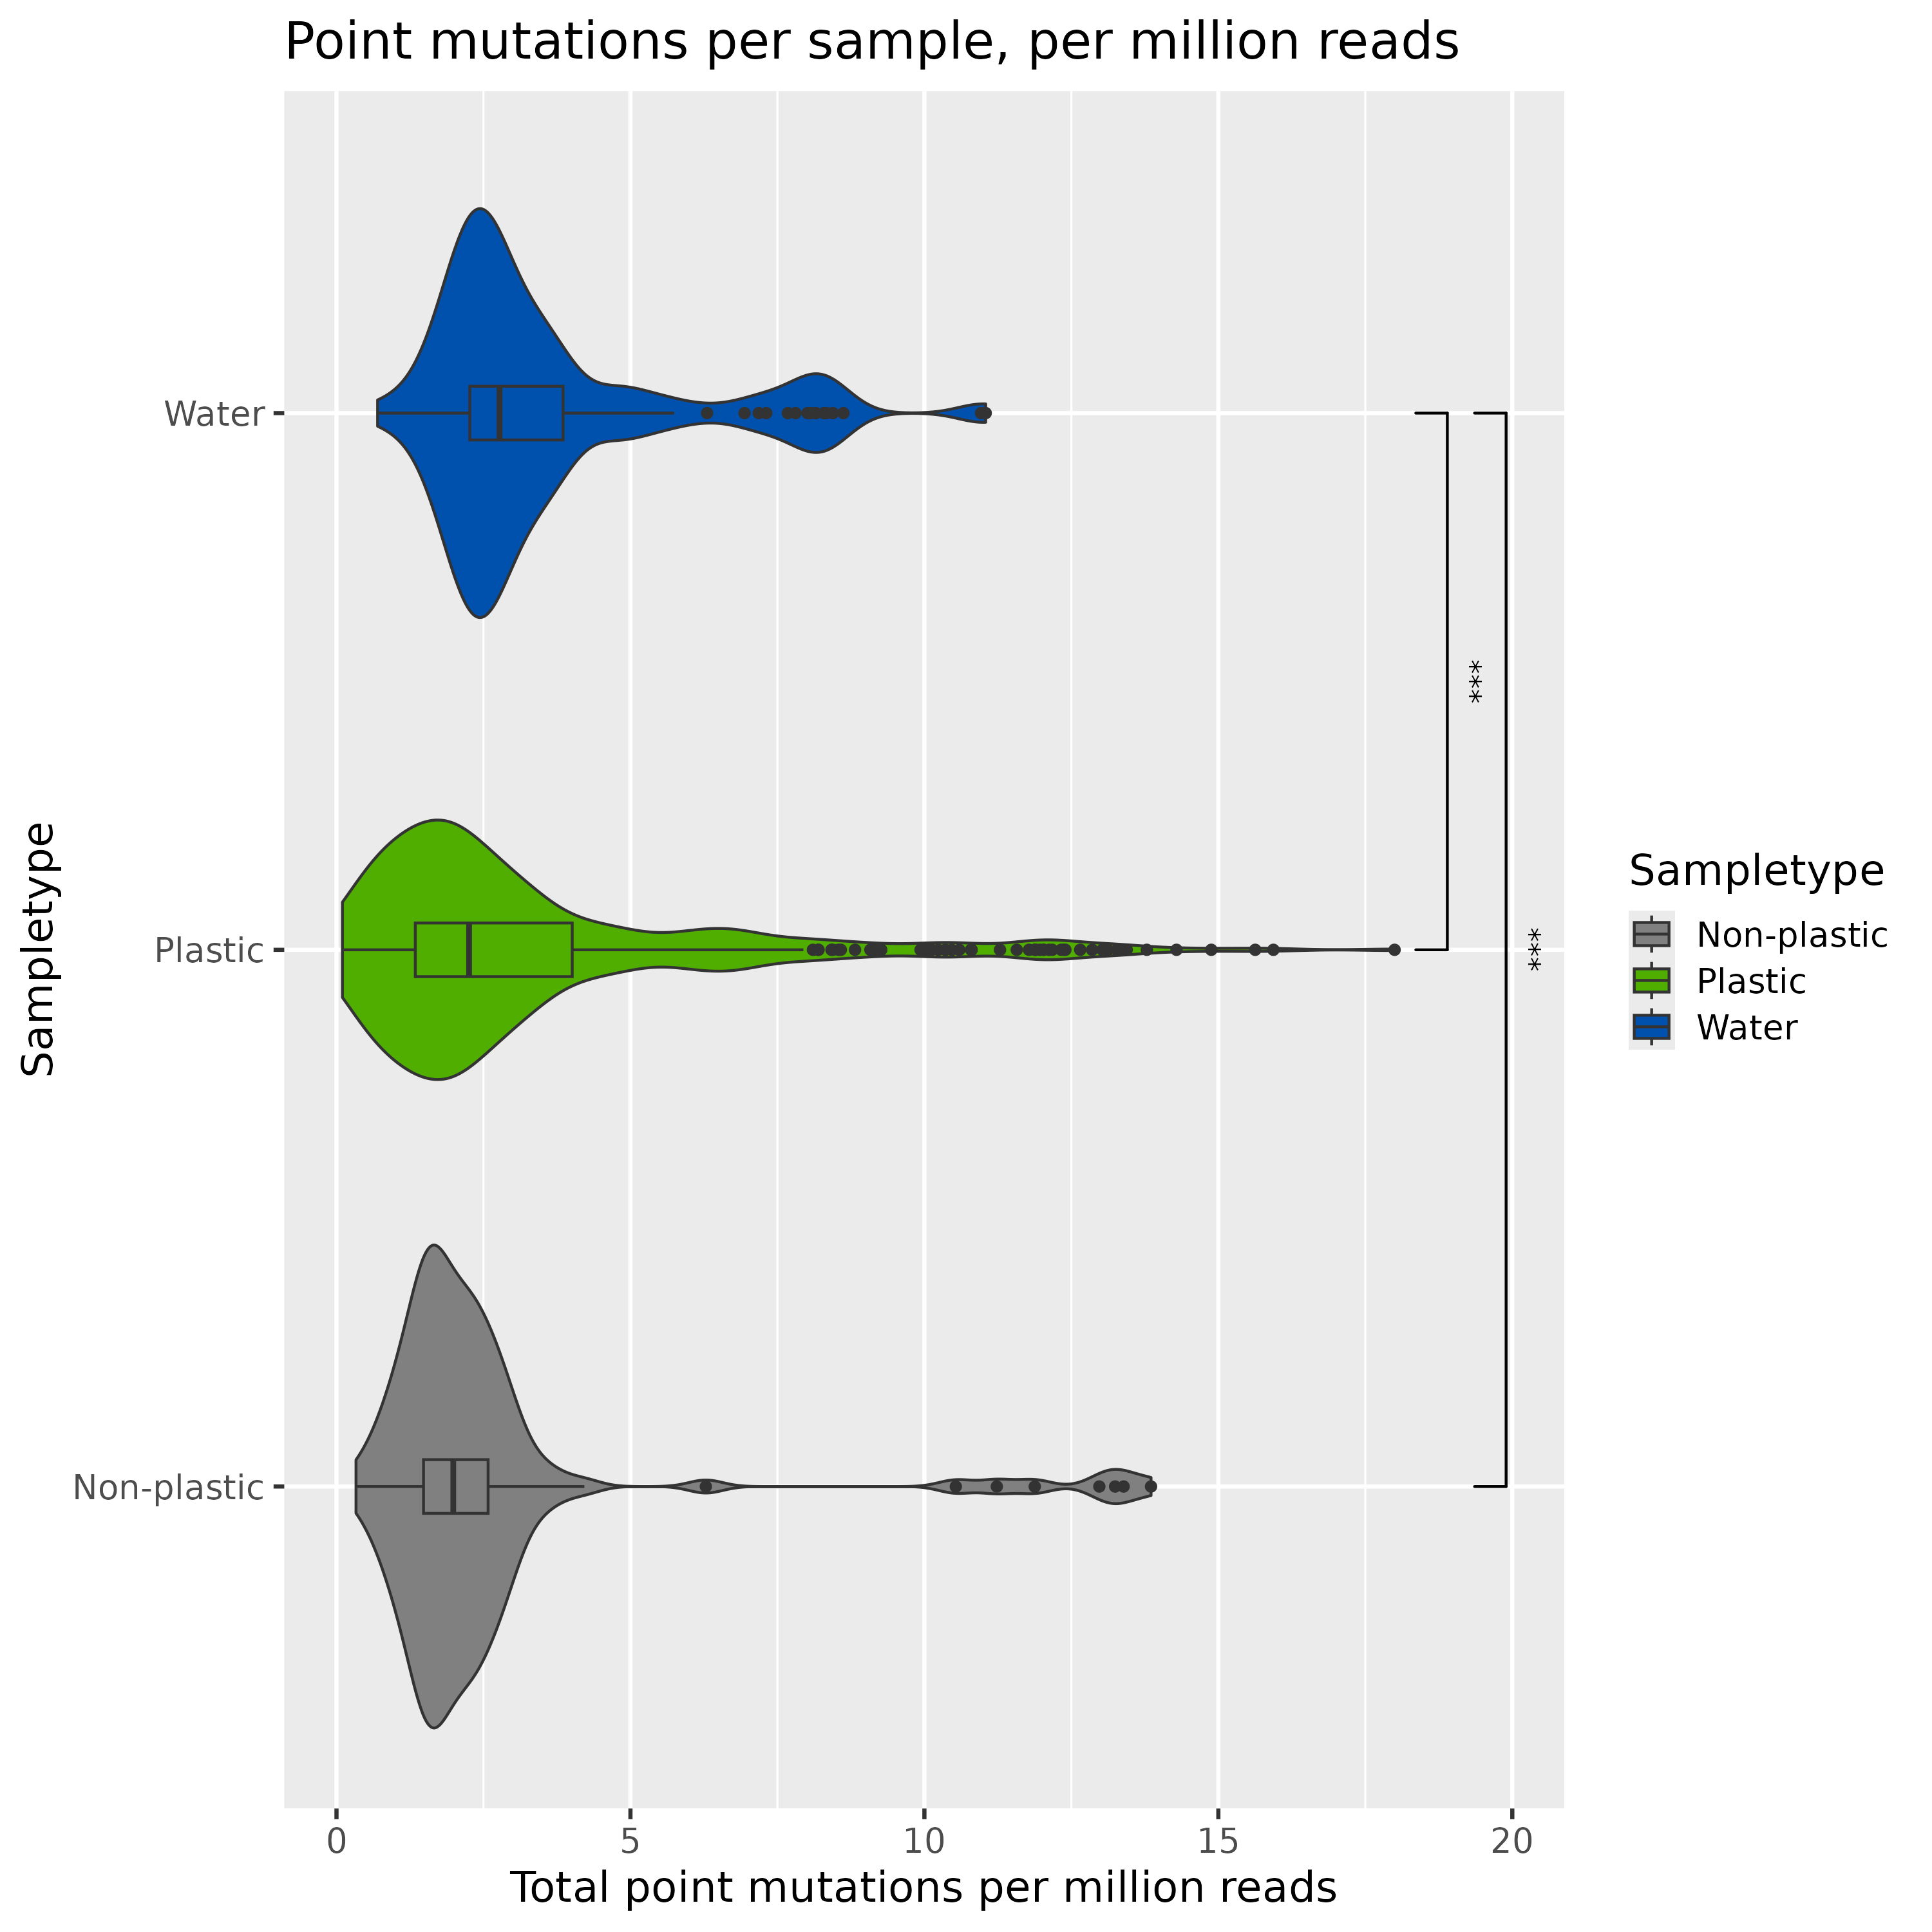
\includegraphics[width = 0.7\textwidth]{figure/hits_per_million_type.png}
    \caption{Total number of mutations per sample, grouped by sampletype. *** = p < 0.001 using Wilcoxon test}
    \label{hits_type}
\end{figure}

%There are also differences when comparing between different substrate types in the same way, as shown in figure \ref{hits_substrate}. The significance of these comparisons are shown in \ref{wilcox_hits_substrate}.
There were differences between the total number of point mutations for different substrate types were compared, as shown in Figure \ref{hits_substrate}, where the significance (from a Wilcoxon test) of these comparisons are shown in \ref{wilcox_hits_substrate}.
The plastic substrates PE-fiber-PE (PFP), Ecovio, and BI-OPL showed an increase (p < 0.05) in the number of point mutations compared to most other substrates. Both Ecovio and BI-OPL are biodegradable plastics, while PFP is not.
High-density polyethylene (HDPE) showed a significant (p < 0.05) decrease in the number of point mutations compared to all other substrates.
%The result of grouping the samples by substrate type instead is shown in figure \ref{hits_substrate}, which show that there was a great difference in total hit count per million between different substrate types. 
%Figure \ref{wilcox_hits_substrate} show the statistical significance of the comparison, where a wilcoxon test was done for the Substrate versus the Reference. The figure also shows the sign of the pseudo-mean for the comparison, labelled "Change", and is set to Increase if the pseudo-mean is positive and Decrease if it negative.
%Note that all comparisons were done, but only the significant ones (p < 0.05) are shown.
%There are some plastic substrates which increased comp ared to most other substrates. These include PFP, Ecovio and BI-OPL. 
The plastic substrates which showed a significant increase compared to any of the water substrates were polyhydroxybutyrate (PHB), PE-fiber (PF), polybutylene adipate terephthalate (PBAT), low-density polyethylene (LDPE), Ecovio, and BI-OPL.
The soil substrate also showed an overall increase in point-mutation rates compared to most other substrates, as did freshwater and seawater, with the exception of PFP, Ecovio, and BI-OPL. 

% Based on the result in these figures, it is evident that the number of point mutations which confer antibiotic resistance are not more prevalent on all plastics, but instead that specific plastic substrates increase this count.
% These substrates include PFP, Ecovio, and BI-OPL. The latter two are biodegradable plastics which contain a blend of PBAT and PLA. 


\begin{figure}[h!]
    \centering
    \subfloat[\label{hits_substrate}]{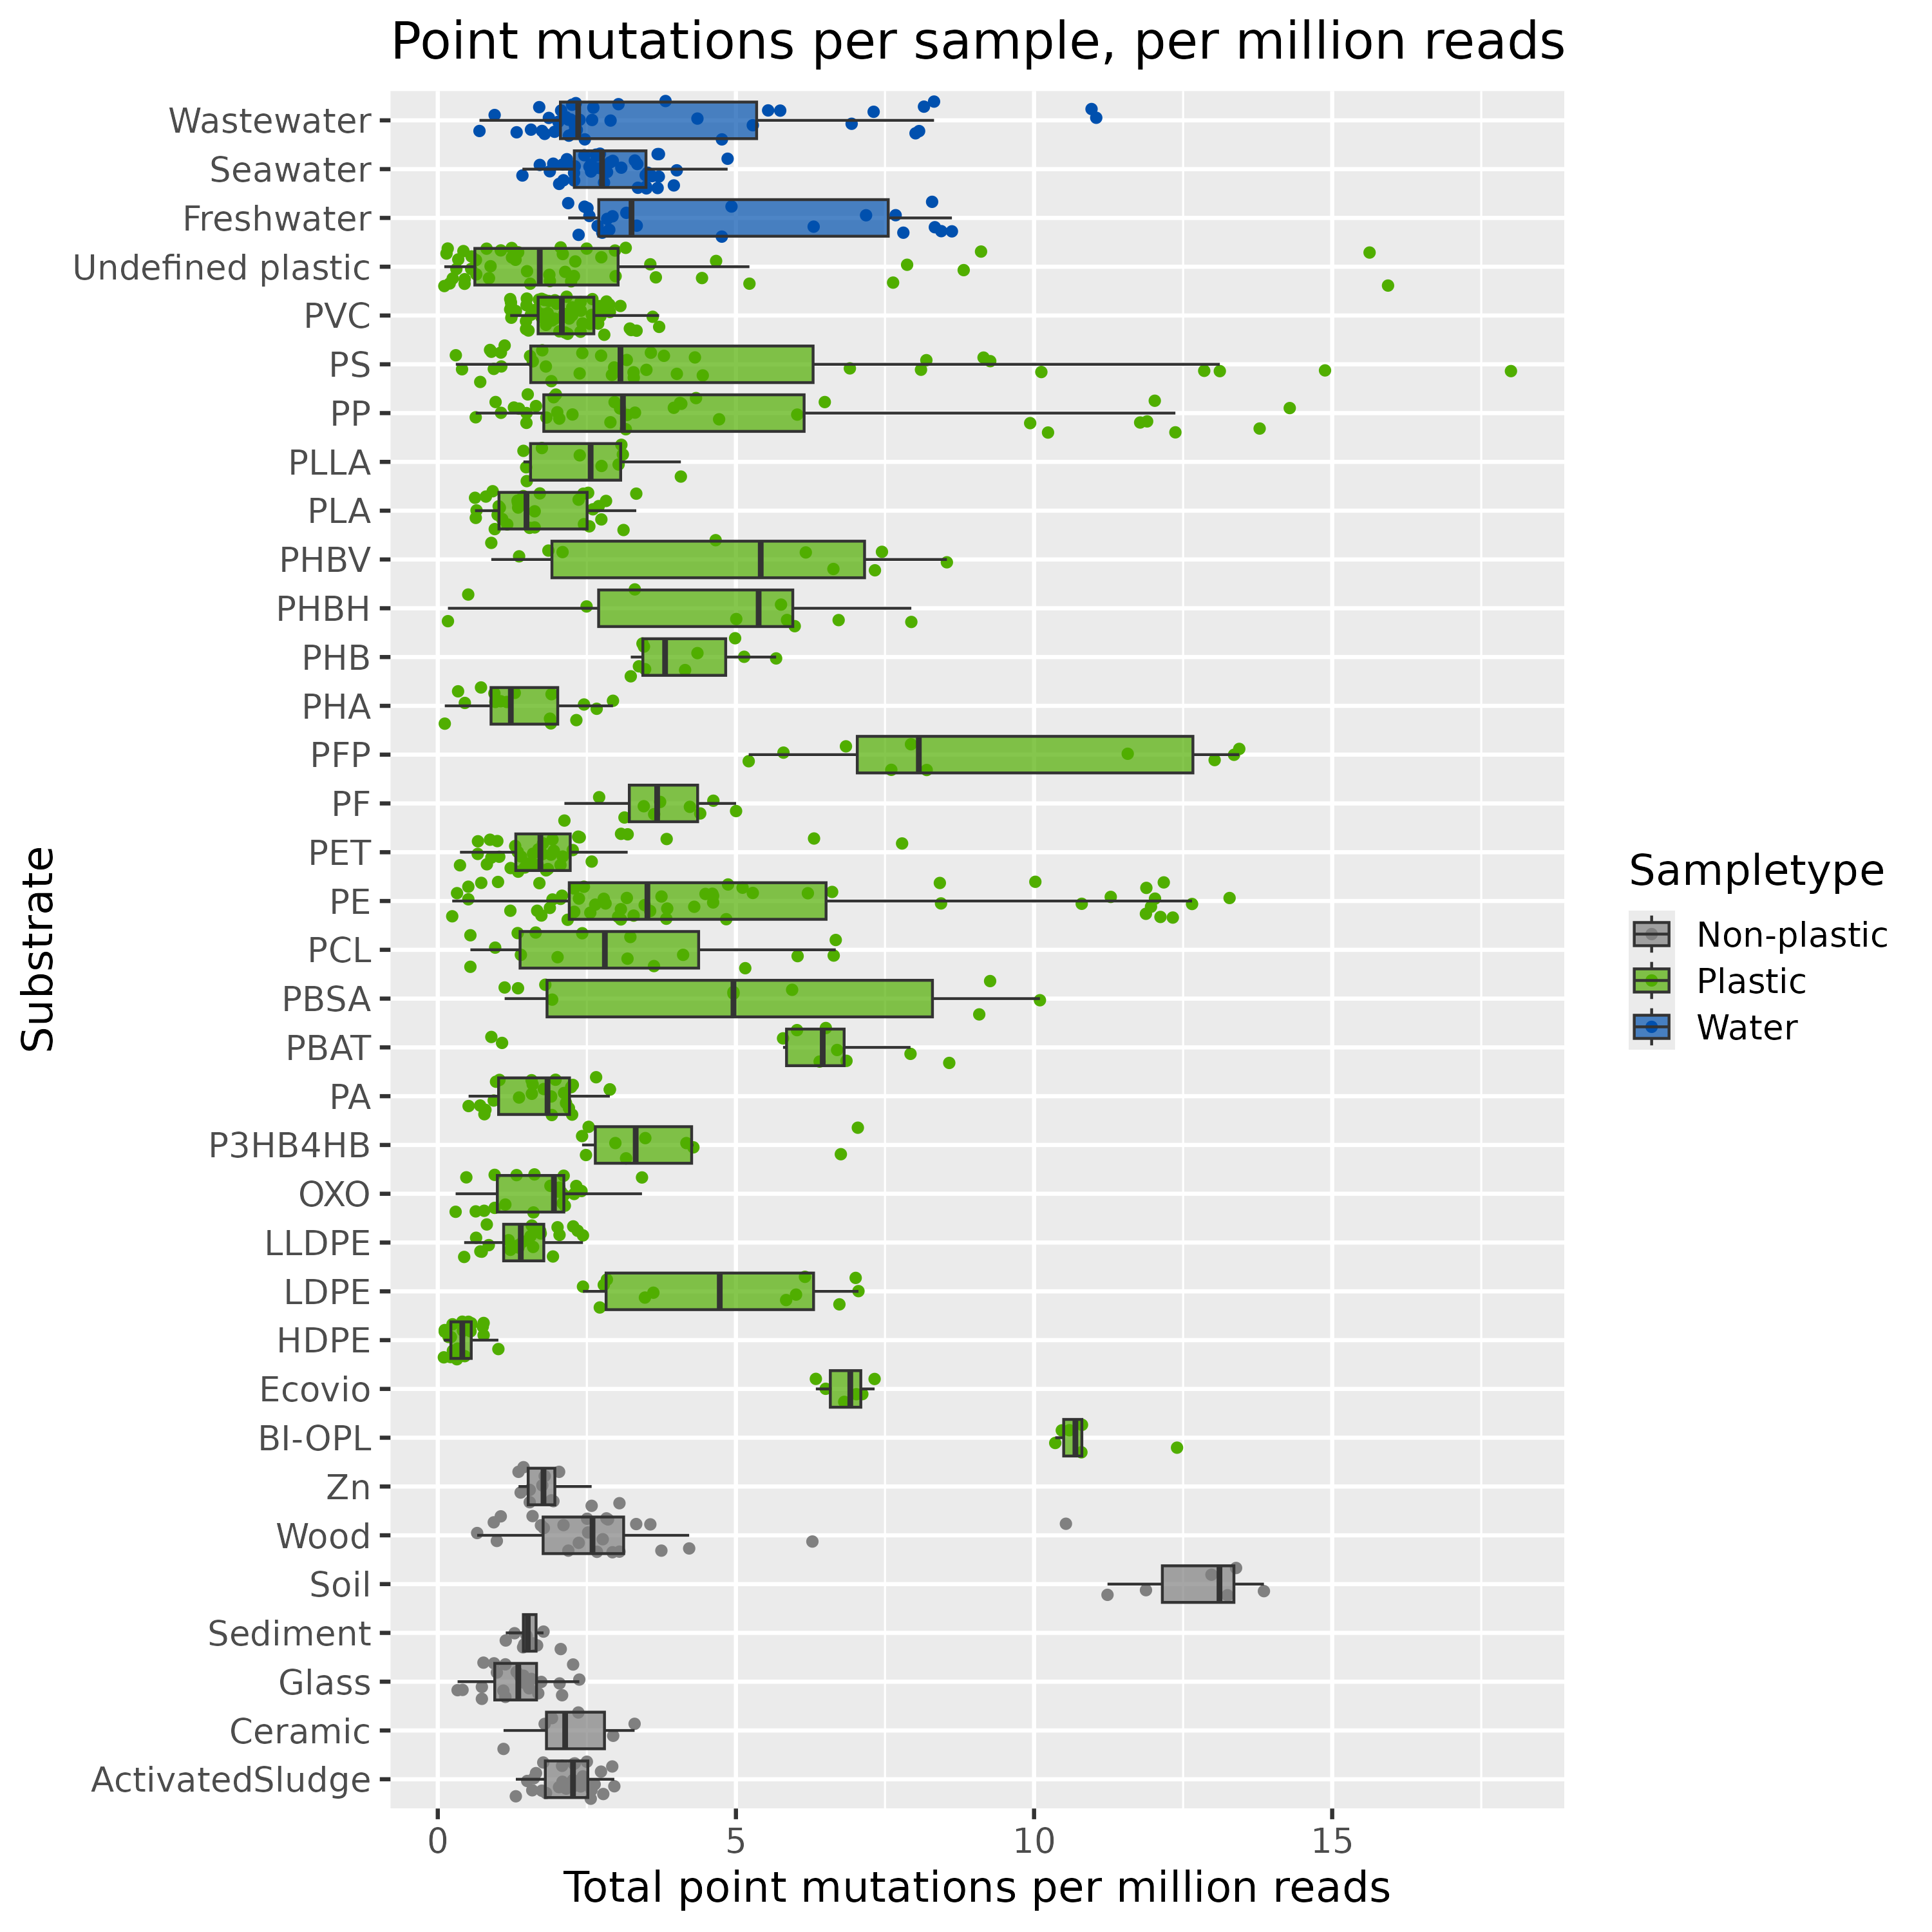
\includegraphics[width=0.5\textwidth]{figure/hits_per_million_substrate.png}}
    \subfloat[\label{wilcox_hits_substrate}]{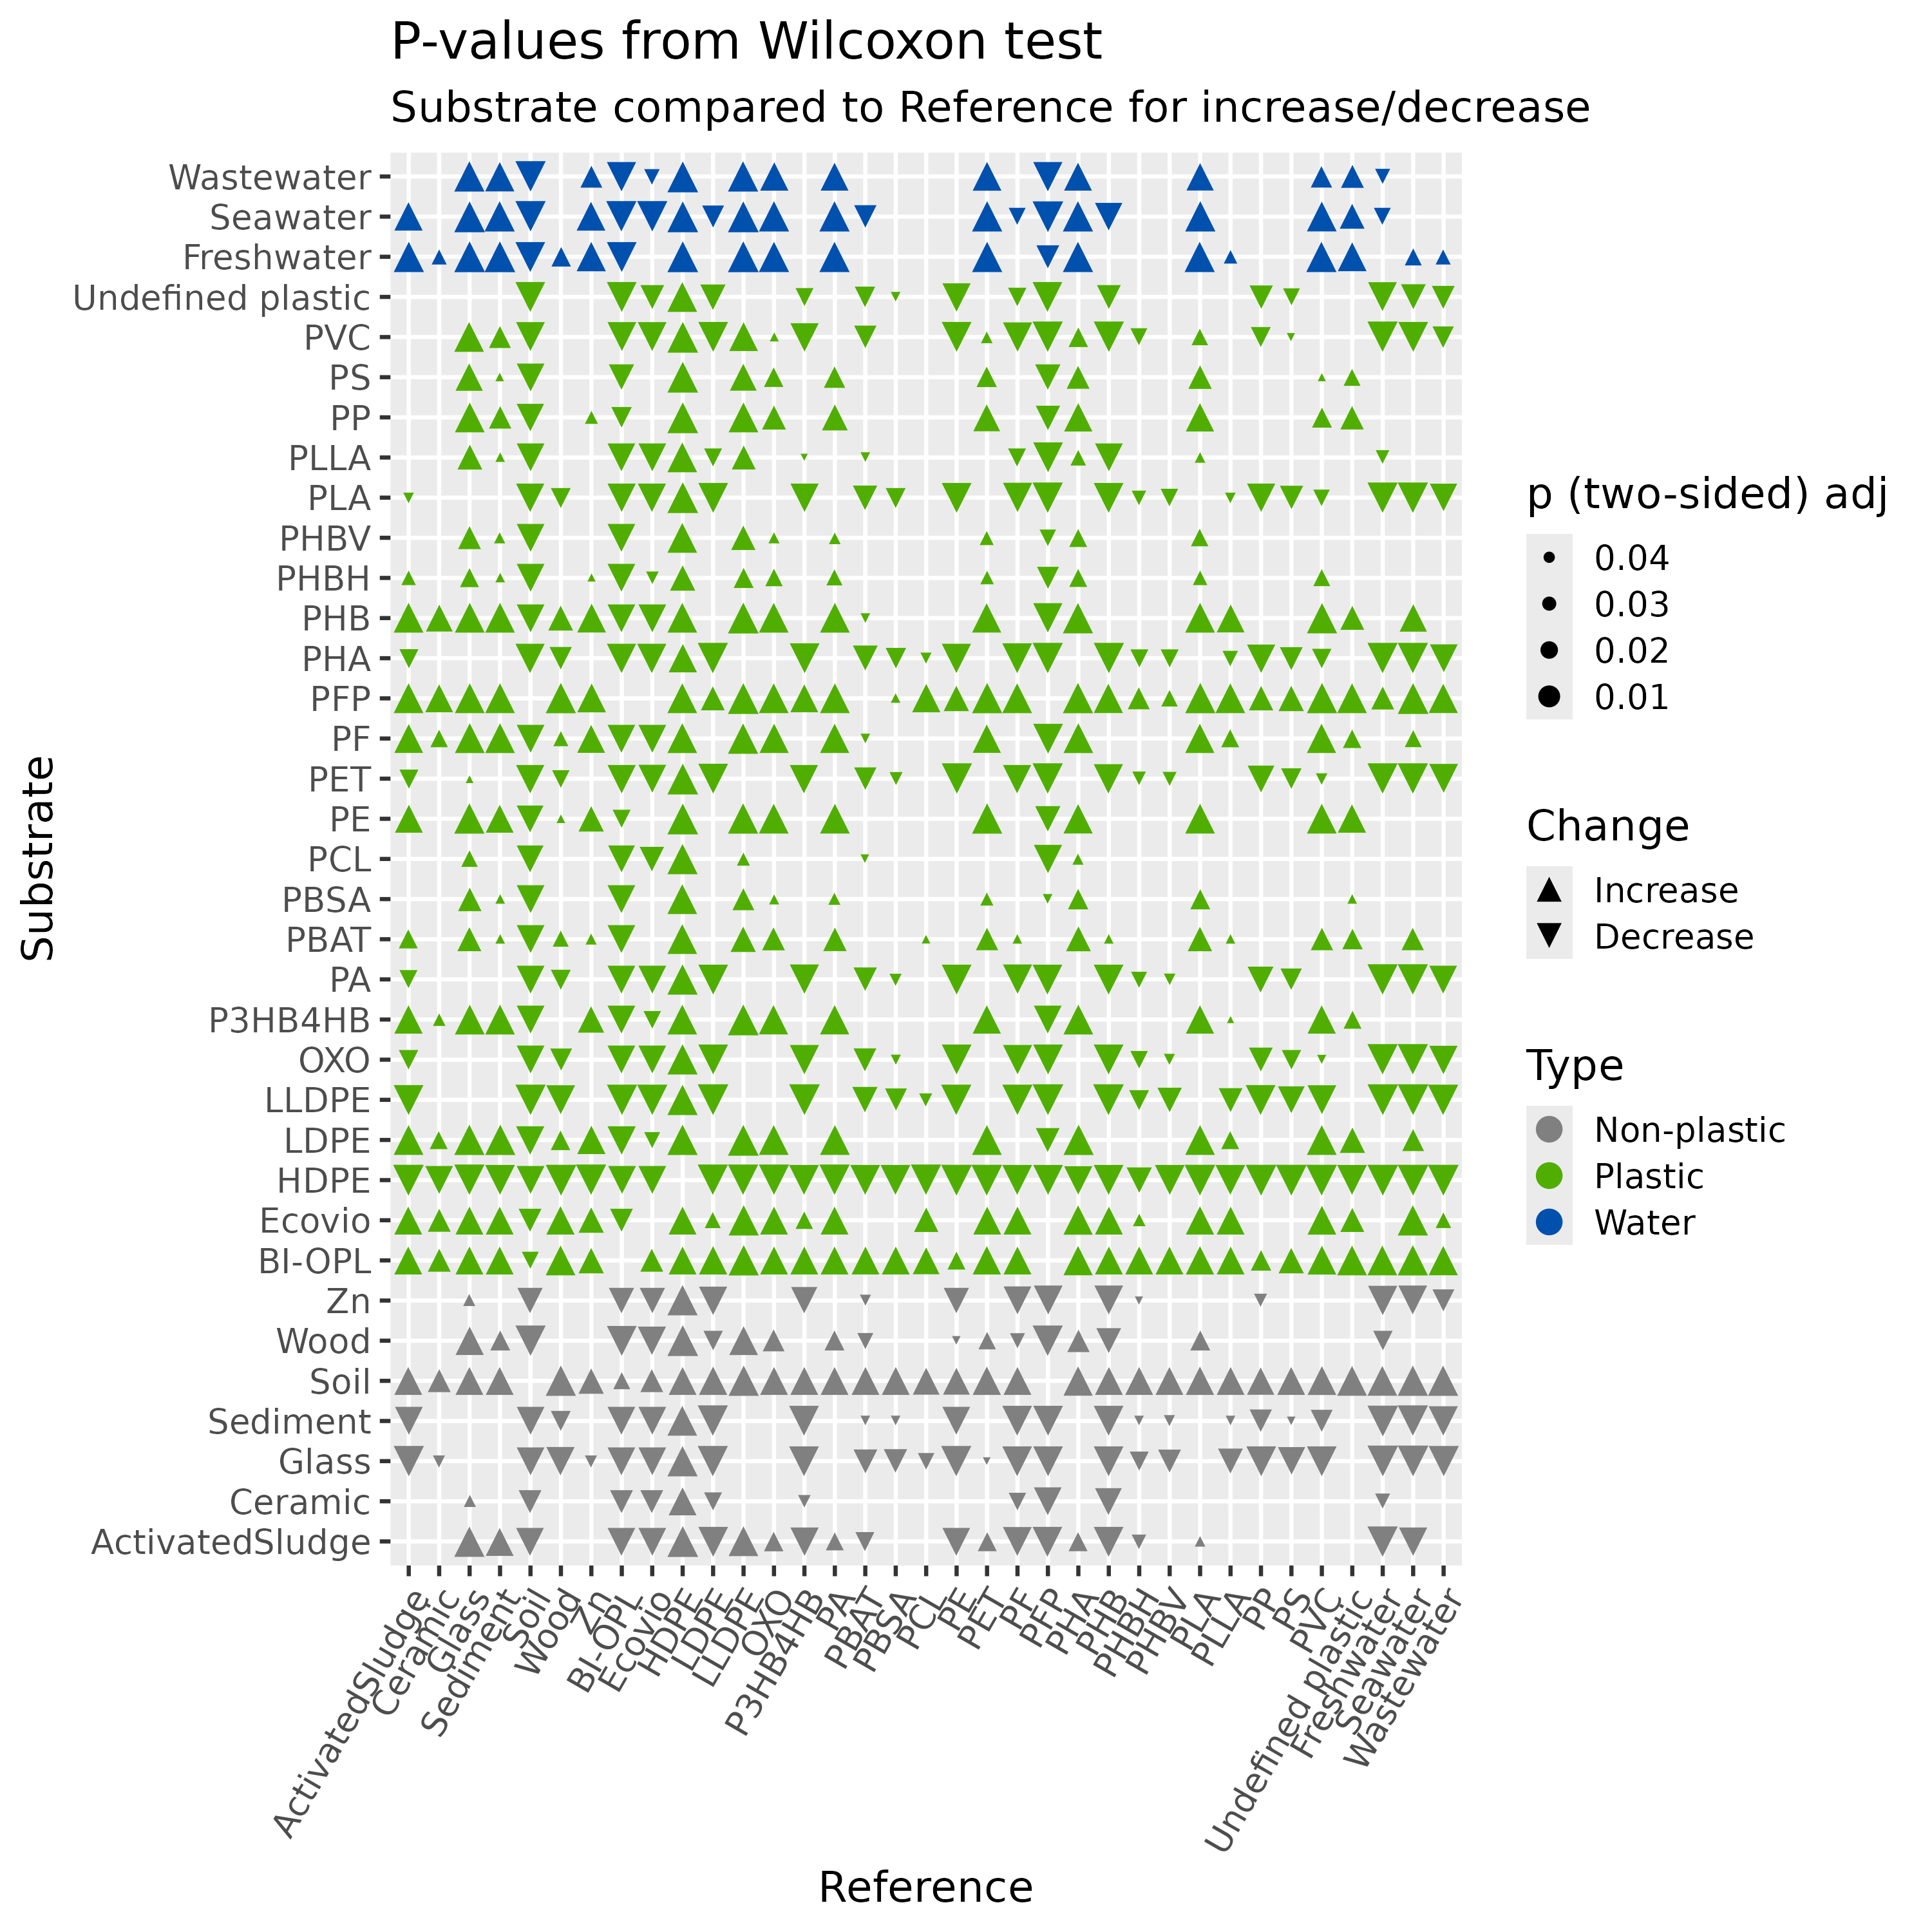
\includegraphics[width=0.5\textwidth]{figure/wilcox_hits_substrates.png}}
    \caption{(a) Point mutations per million reads. (b) p-values from Wilcoxon test for the number of point mutations of Subtrate versus Reference. * = p < 0.05, *** = p < 0.001 using Wilcoxon test. Shows only comparisons with p < 0.05, but all comparisons were done. Increase or decrease of pseudomean compared to the reference is shown using point shape}
    \label{both_hits_substrate}
\end{figure}


\section{Mean mutation percentage}
%todo{Mention how the samples are collected, that they take the biofilm and sequence that? Check in a study what they do}
The following section present the results of using the mean mutation percentage instead of the total number of point mutations.
This method has the advantage of reducing the impact of genes with high read coverage, instead using the relative mutation frequency of each individual gene.
The mean mutation percentage was calculated in two different ways.
The first method calculated the mean of the relative mutation percentage of all mutations in each sample.
The second method calculated the mean mutation percentage of each individual point mutation across all samples in each substrate.
When the mean was calculated for the different samples, it estimates the proportion of mutated genes in the sample.
When the mean was instead calculated for the individual point mutations, it estimates how broadly the mutation rate of a point mutation is distributed across samples. 
%As described above this mean value can be calculated for either the samples or the mutations. These values tell you different things, where in the first case it estimates how mutated the genes are in the samples, i.e. "this sample has a mean mutation percentage of 3\%".
%In the latter case it estimates how mutated specific genes are in the different substrates, i.e. "mutation A has a mean mutation percentage of 25\% in freshwater".
% The advantage of this approach is that the relative mutation frequency of the gene is used instead of the total number of point mutations, which normalizes the mutation rate and reduces the impact of genes which a large number of reads map to.

%\subsection{Mean mutation percentage of samples} 
%\subsubsection{Alternative 1, combined plots, otherwise two separate larger plots, see \ref{mean_samples_substrate_full} and \ref{wilcox_samples_substrates_full}}
%The mean mutation percentage was calculated for every sample, and 

Figure \ref{mean_samples_sampletype} show the mean mutation percent grouped by the type of sample.
There was a significant difference (Wilcoxon test: p < 0.001) between the water group and the plastic group, where the plastic group has a lower mean mutation percentage in comparison to the water group(pseudomean: -0.20). None of the other groups displayed any significant difference (Wilcoxon test: p > 0.05) between them.

%\todo{Remove n.s.?}
\begin{figure}[h!]
    \centering
    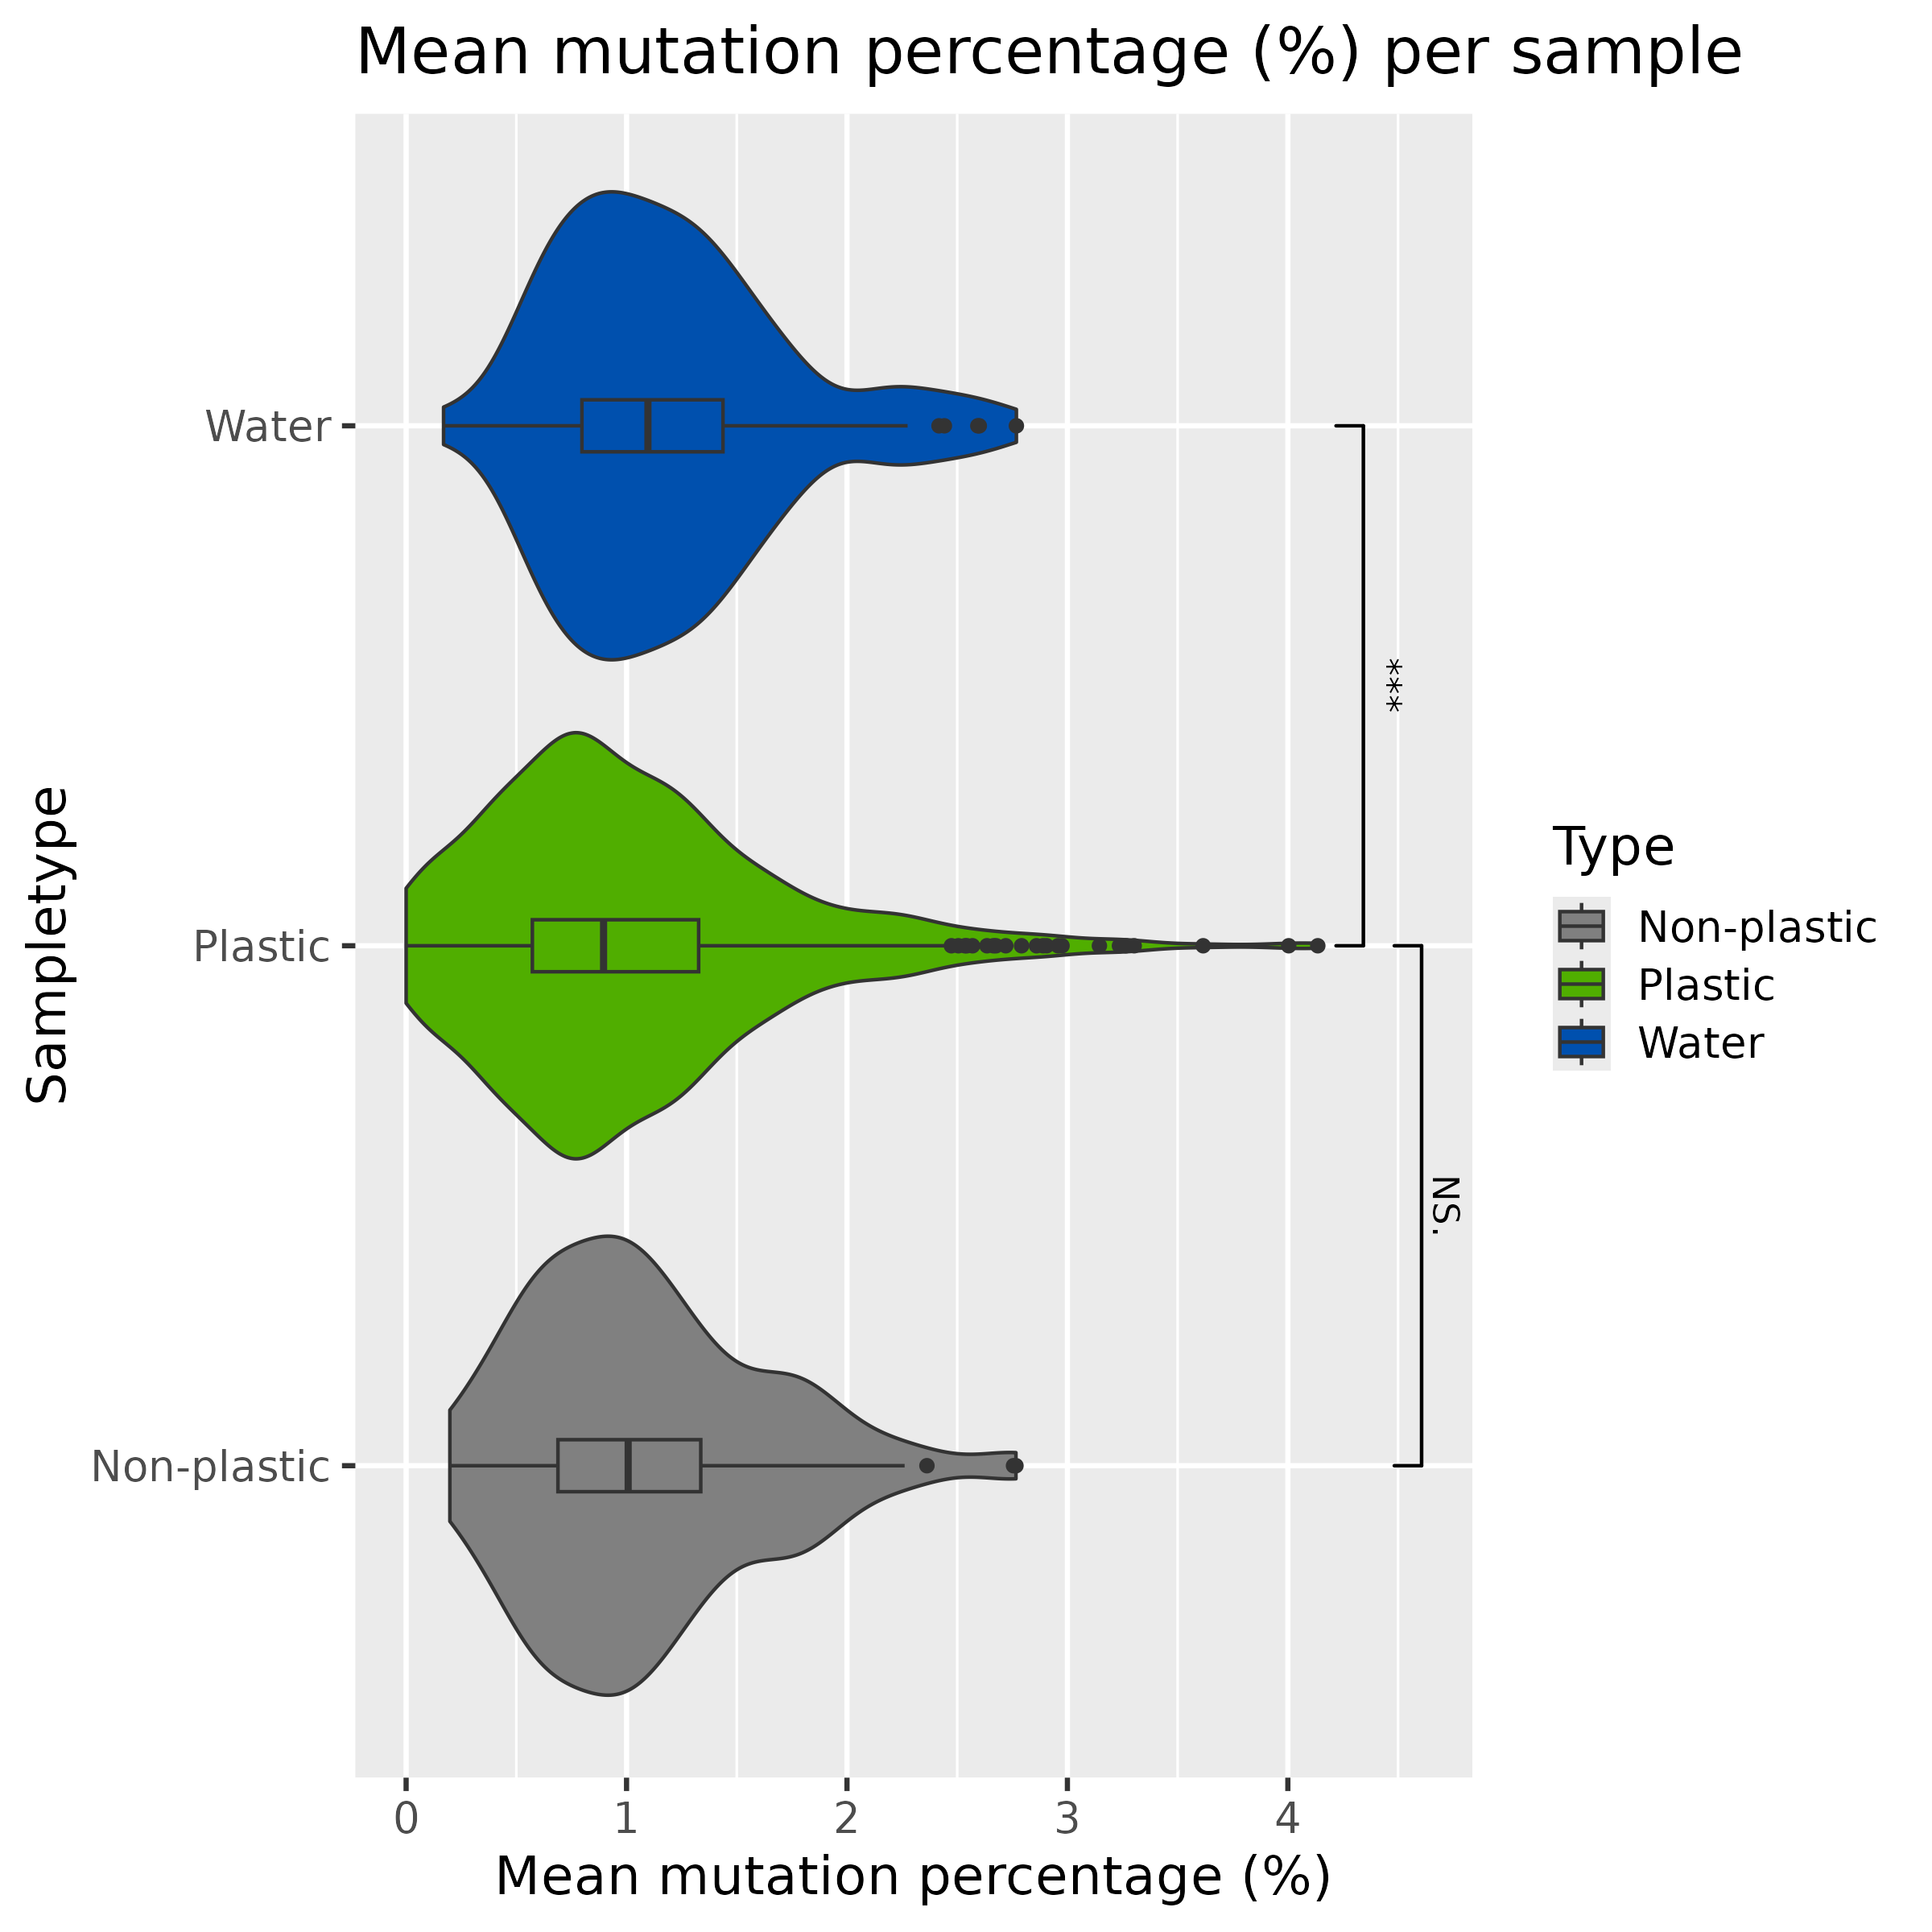
\includegraphics[width = 0.6\textwidth]{figure/mean_samples_sampletype.png}
    \caption{Mean mutation percentage (\%) per sample, grouped by sampletype. *** = p < 0.001 using Wilcoxon test.}
    \label{mean_samples_sampletype}
\end{figure}
%\todo{P-values-table in appendix or not at all?)}

% \begin{table}[h]
% \caption{p-values from Wilcoxon test between sampletypes}
% \label{wilcox_samples_sampletype}
% \begin{tabular}{@{}llllll@{}}
% \toprule
% Sampletype A & Sampletype B & Significance & Change   & p (two-sided) & pseudo\_mean  \\ \midrule
% Non-plastic  & Plastic      & *            & Increase & 0.0473  &  0.0012  \\
% Water        & Plastic      & ***          & Increase & 0.0005  &  0.0020  \\
% Non-plastic  & Water        & ns           & Decrease & 0.1801  & -0.0009 \\
% Plastic      & Water        & ***          & Decrease & 0.0005  & -0.0020 \\
% Plastic      & Non-plastic  & *            & Decrease & 0.0473  & -0.0012 \\
% Water        & Non-plastic  & ns           & Increase & 0.1801  &  0.0009 \\ \bottomrule
% \end{tabular}
% \end{table}

%In figure \ref{mean_samples_substrate} the samples were instead grouped by substrate type, which shows that there were differences for different plastics, as well as other substrates.
There were differences between the different plastics and other substrates when the samples were instead grouped by sample type as shown in Figure \ref{mean_samples_substrate}.
There were some plastics that had a significantly higher mean mutation percentage than most other substrates, which included PFP, LDPE, Ecovio and BI-OPL. The last two plastics are biodegradable plastics.
The plastic substrates that had a significantly higher mean mutation percentage than seawater or wastewater included polyvinyl chloride (PVC) and PF in addition to PFP, LDPE, Ecovio and BI-OPL.
There were also some plastics which had significantly lower mean mutation percentage than almost all other substrates, the most notable of which was high-density polyethylene (HDPE), poly(3-hydroxybutyrate-co-3-hydroxyvalerate) (PHBV) and polyhydroxyalkanoate (PHA), of which the last two are biodegradable polymers.
Almost all substrates had a significantly lower mean mutation percentage than the freshwater samples and the soil samples, the exception of which was Ecovio, BI-OPL, and PFP where there was no significant (p < 0.05) difference. 
%The soil samples have a significantly higher (p < 0.001) mean mutation percentage compared to most other substrates. 
%todo{meh, "which is expected from previous studies" + ref? Idk varför det nämns}.


\begin{figure}[h!]
    \centering
    \subfloat[\label{mean_samples_substrate}]{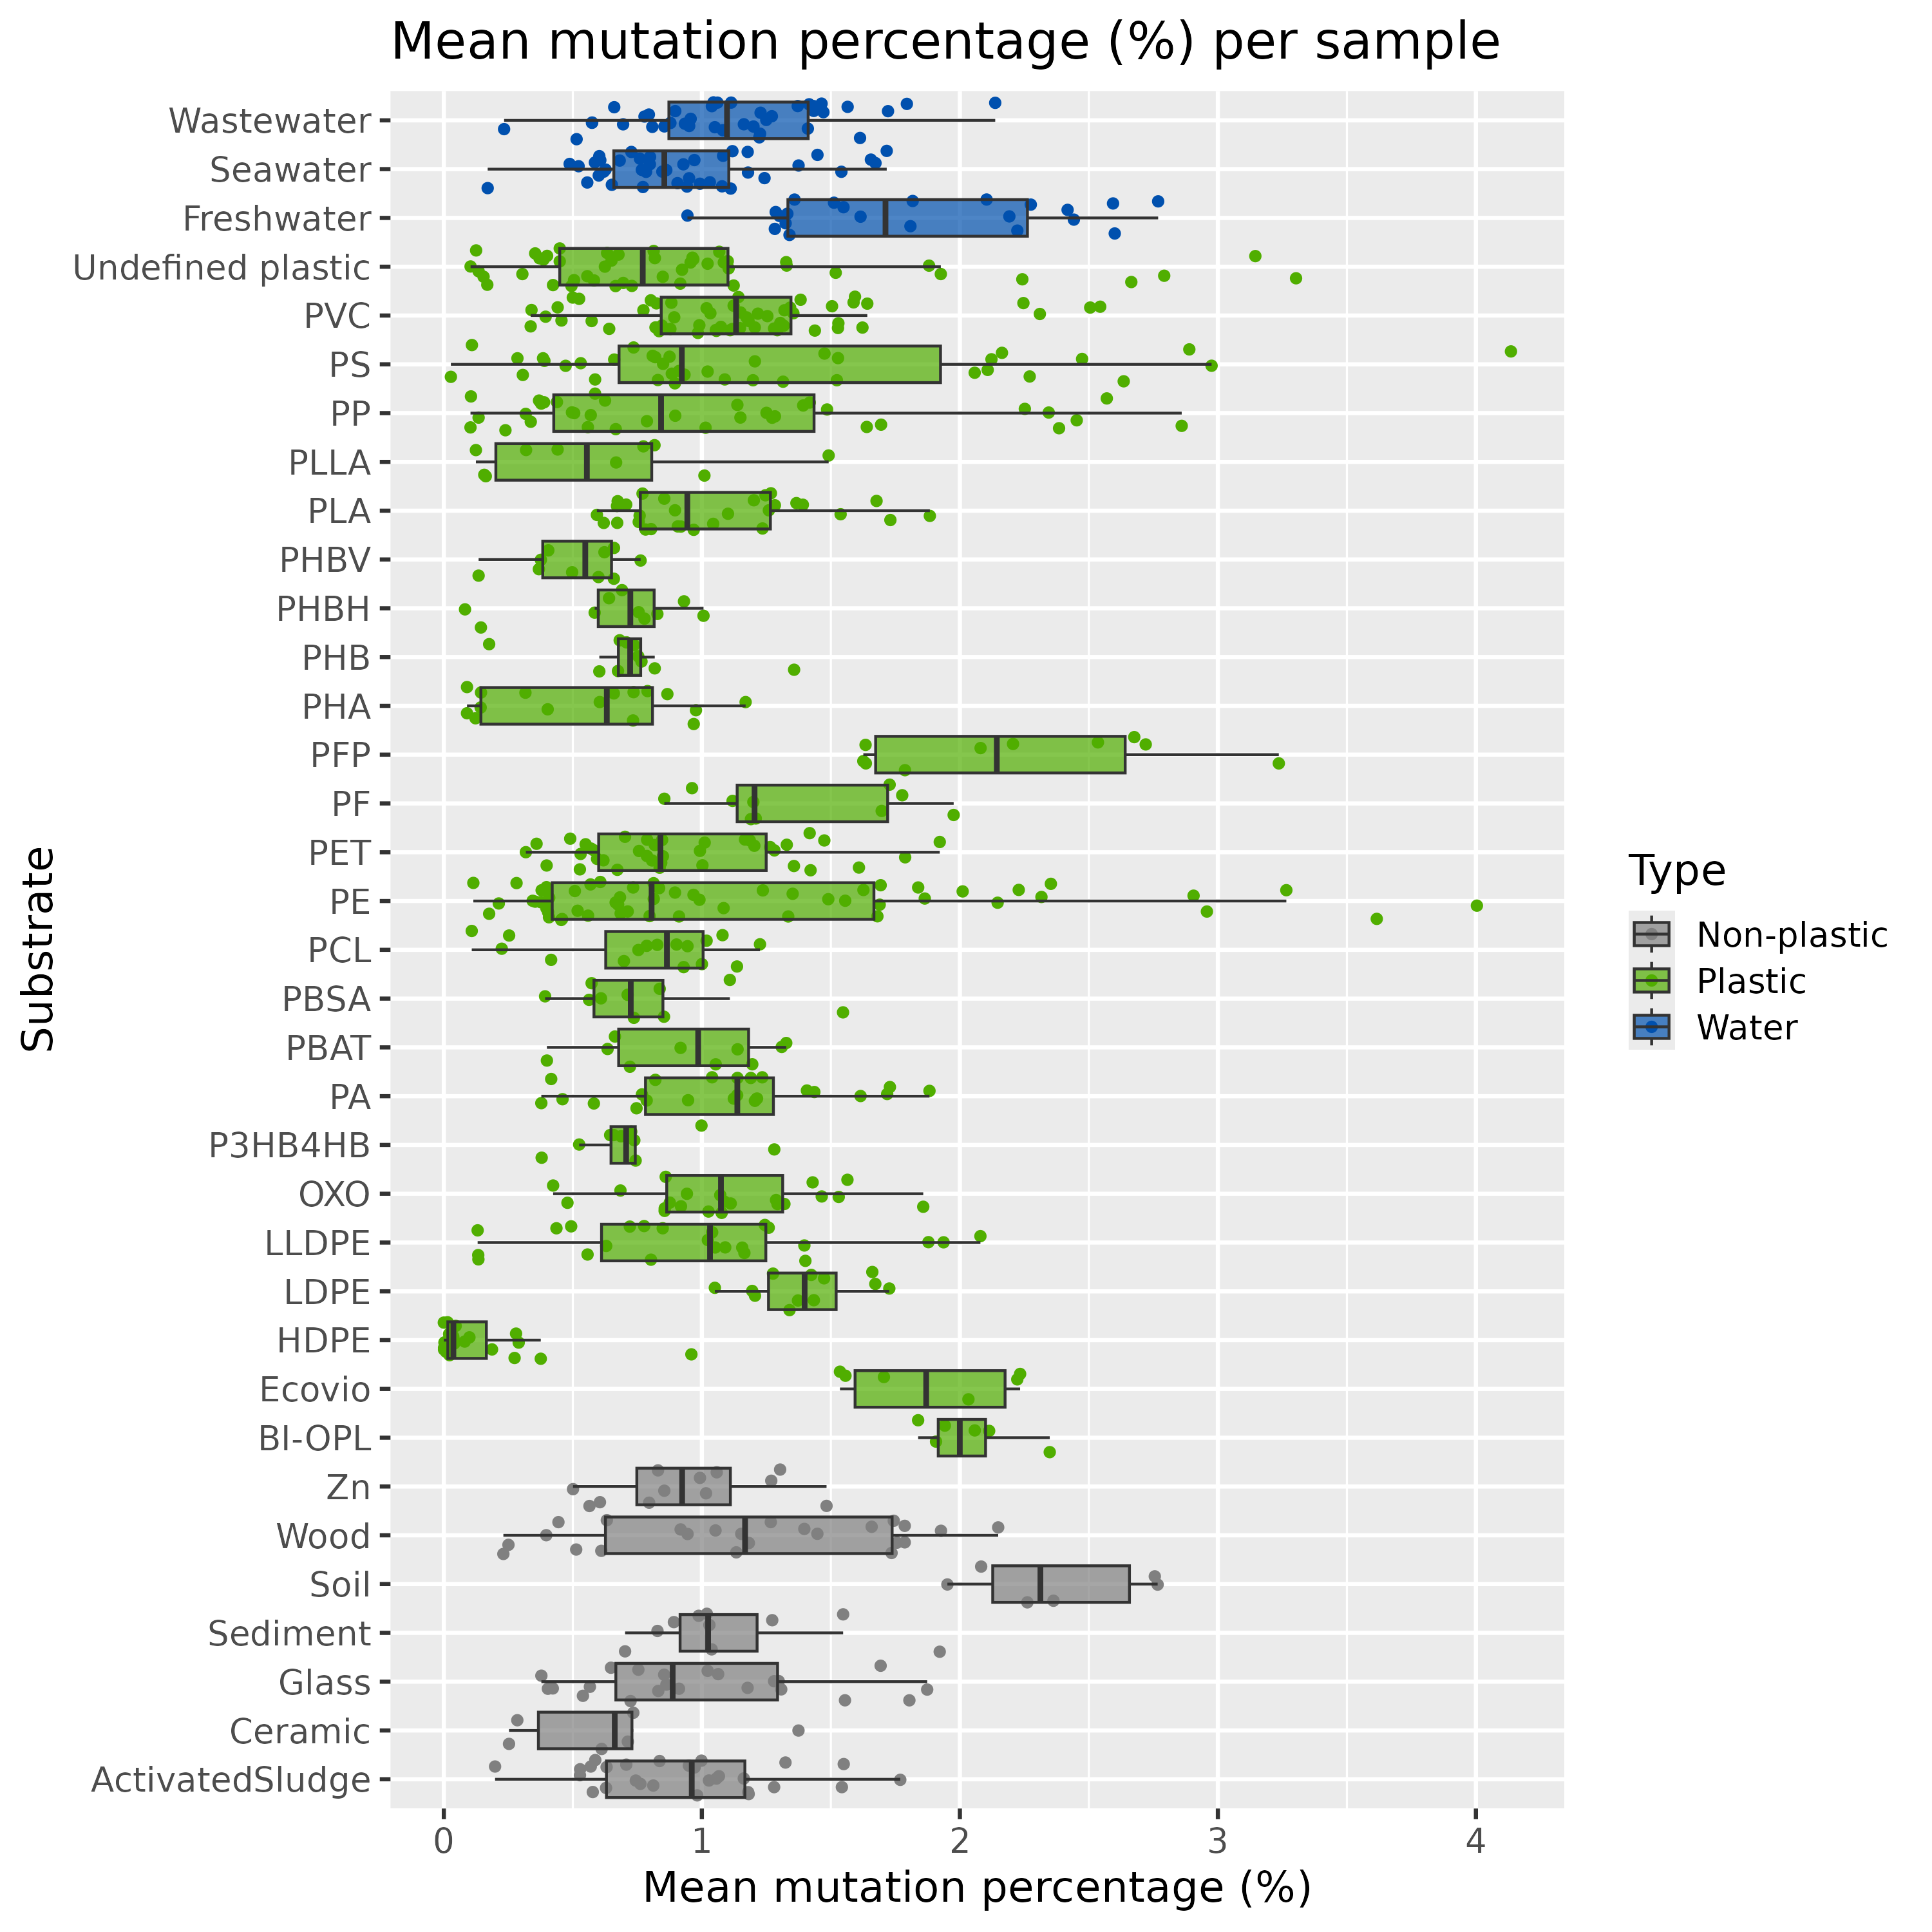
\includegraphics[width=0.5\textwidth]{figure/mean_samples_substrate.png}}
    \subfloat[\label{wilcox_samples_substrate}]{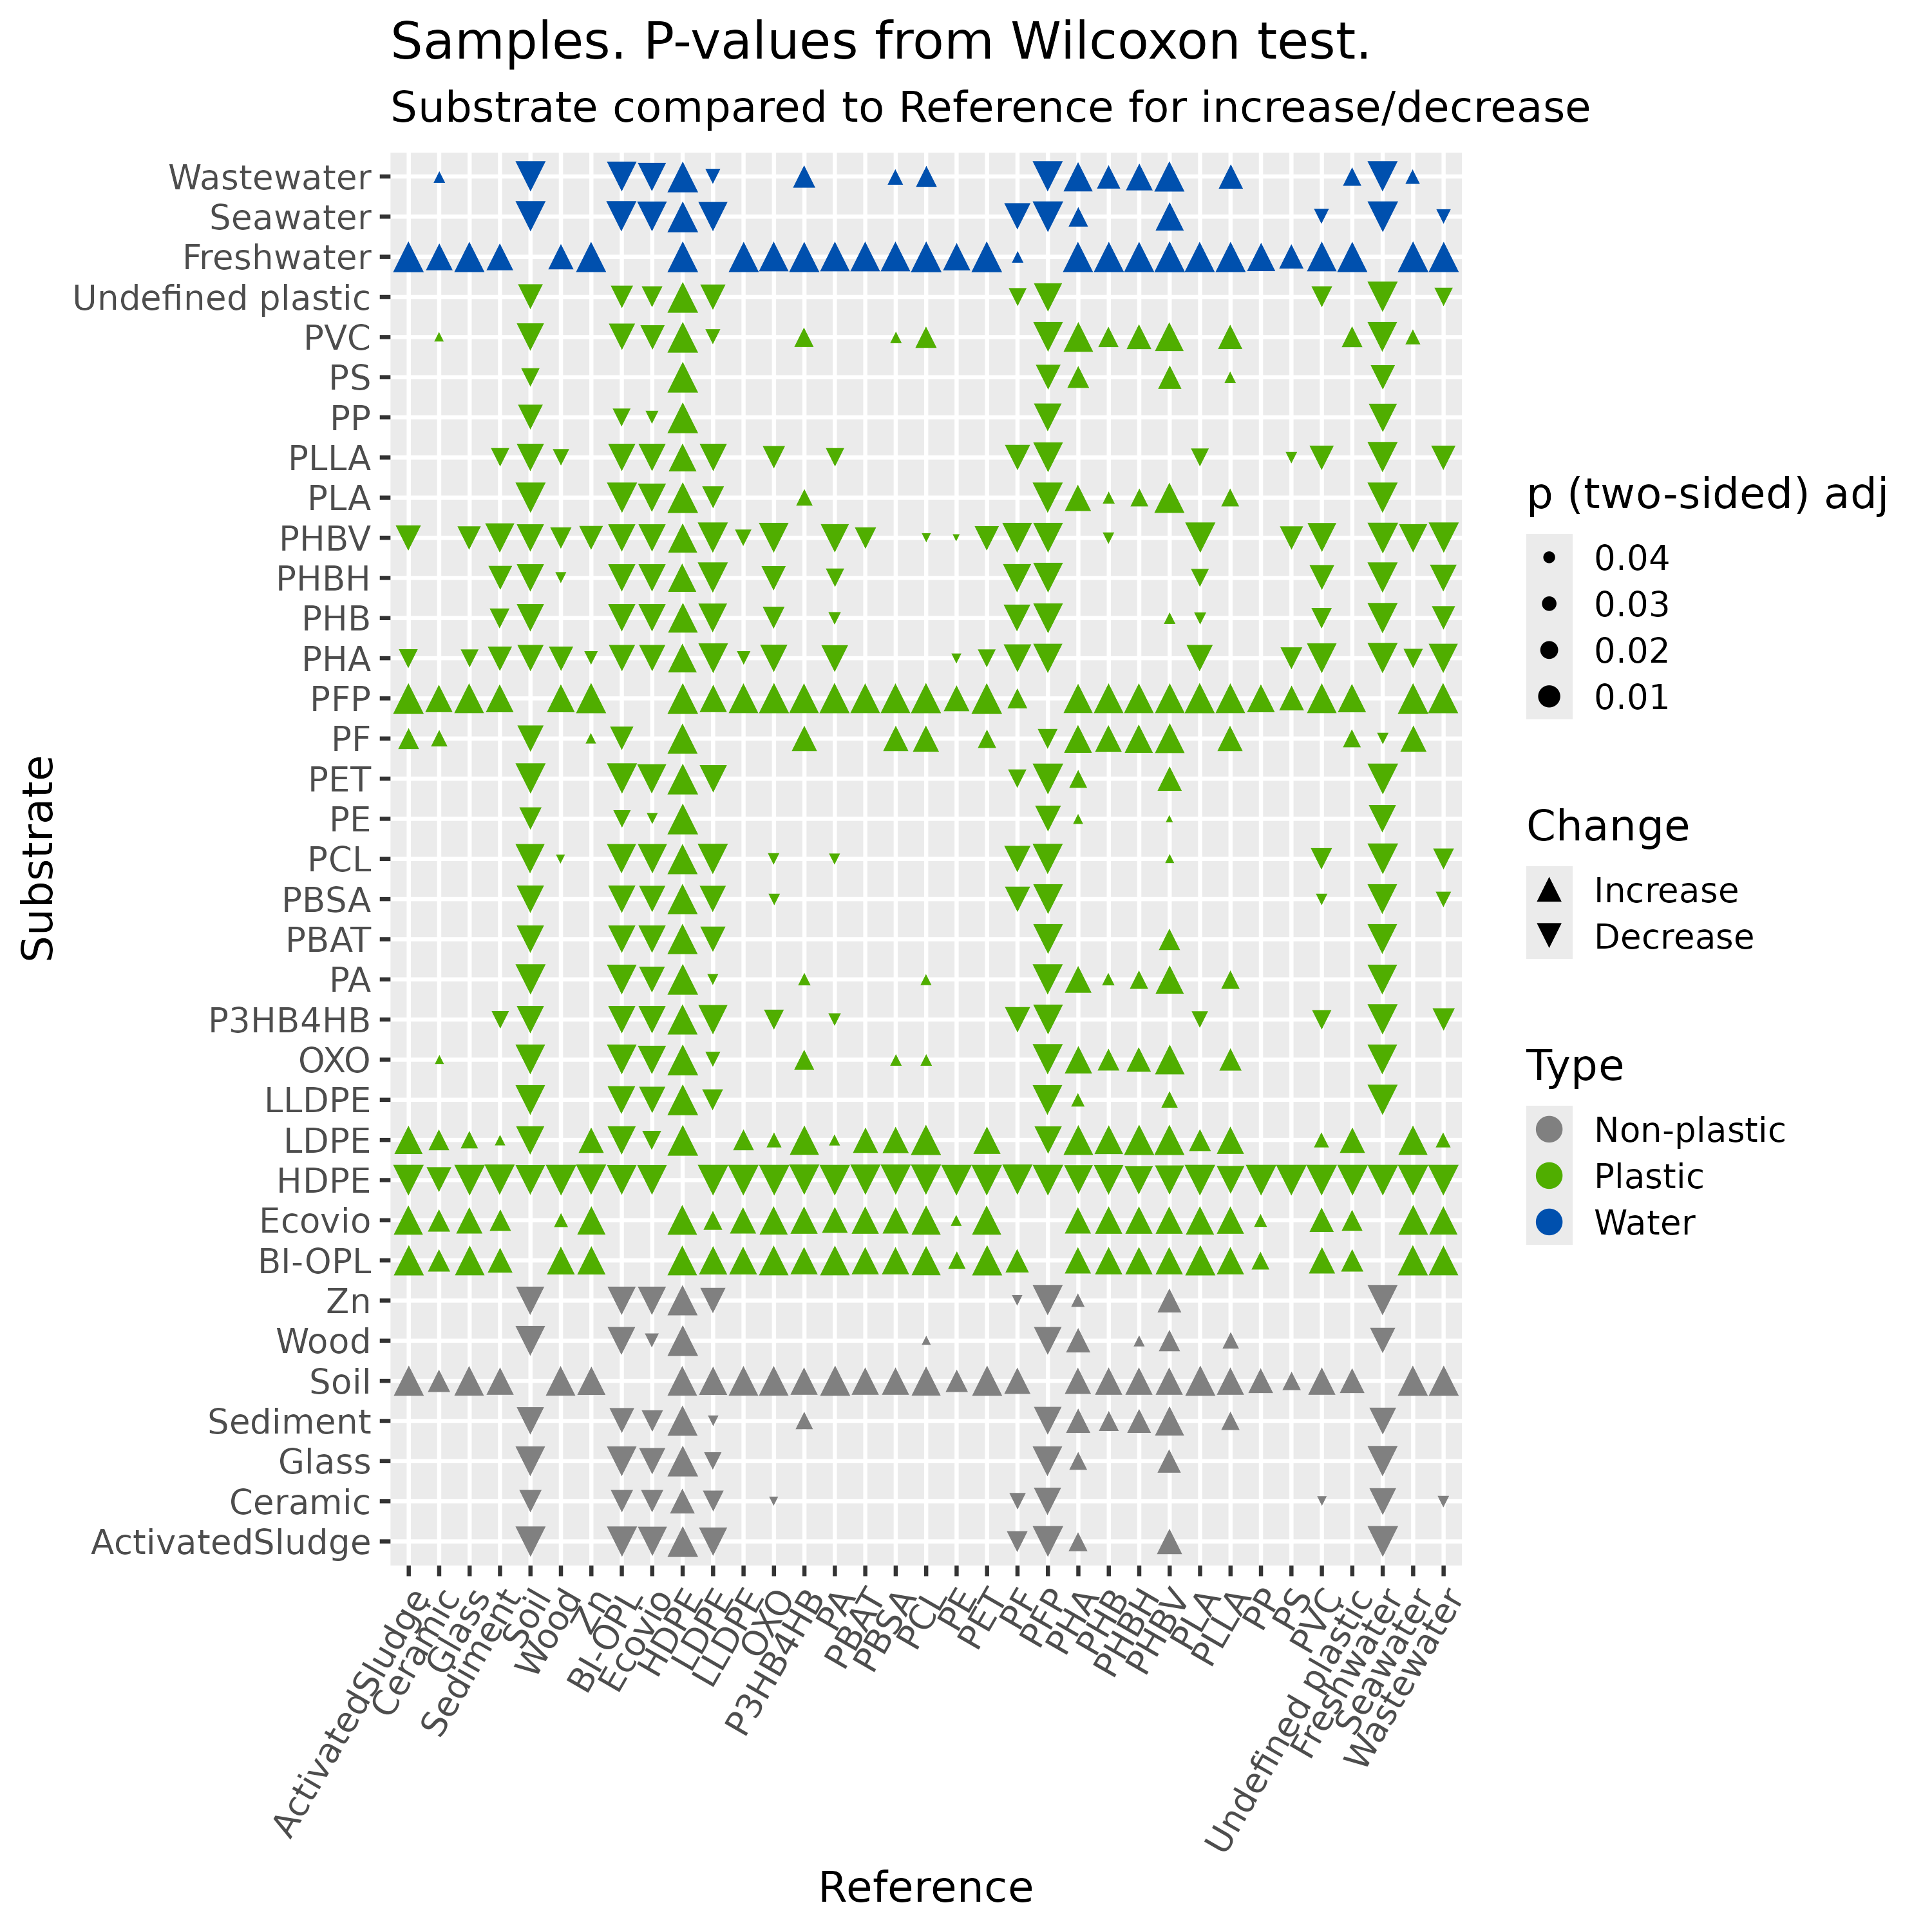
\includegraphics[width=0.5\textwidth]{figure/wilcox_samples_substrates.png}}
    \caption{(a) Mean mutation percentage per sample, grouped by substrate type. (b) p-values from Wilcoxon test of mean mutation percentage for Substrate versus Reference}
    \label{both_mean_samples_susbtrates}
\end{figure}

%\subsubsection{Alternative 2, separate plots instead of combined, see figure \ref{both_mean_samples_susbtrates}}
%\begin{figure}[h]
    % \centering
    % 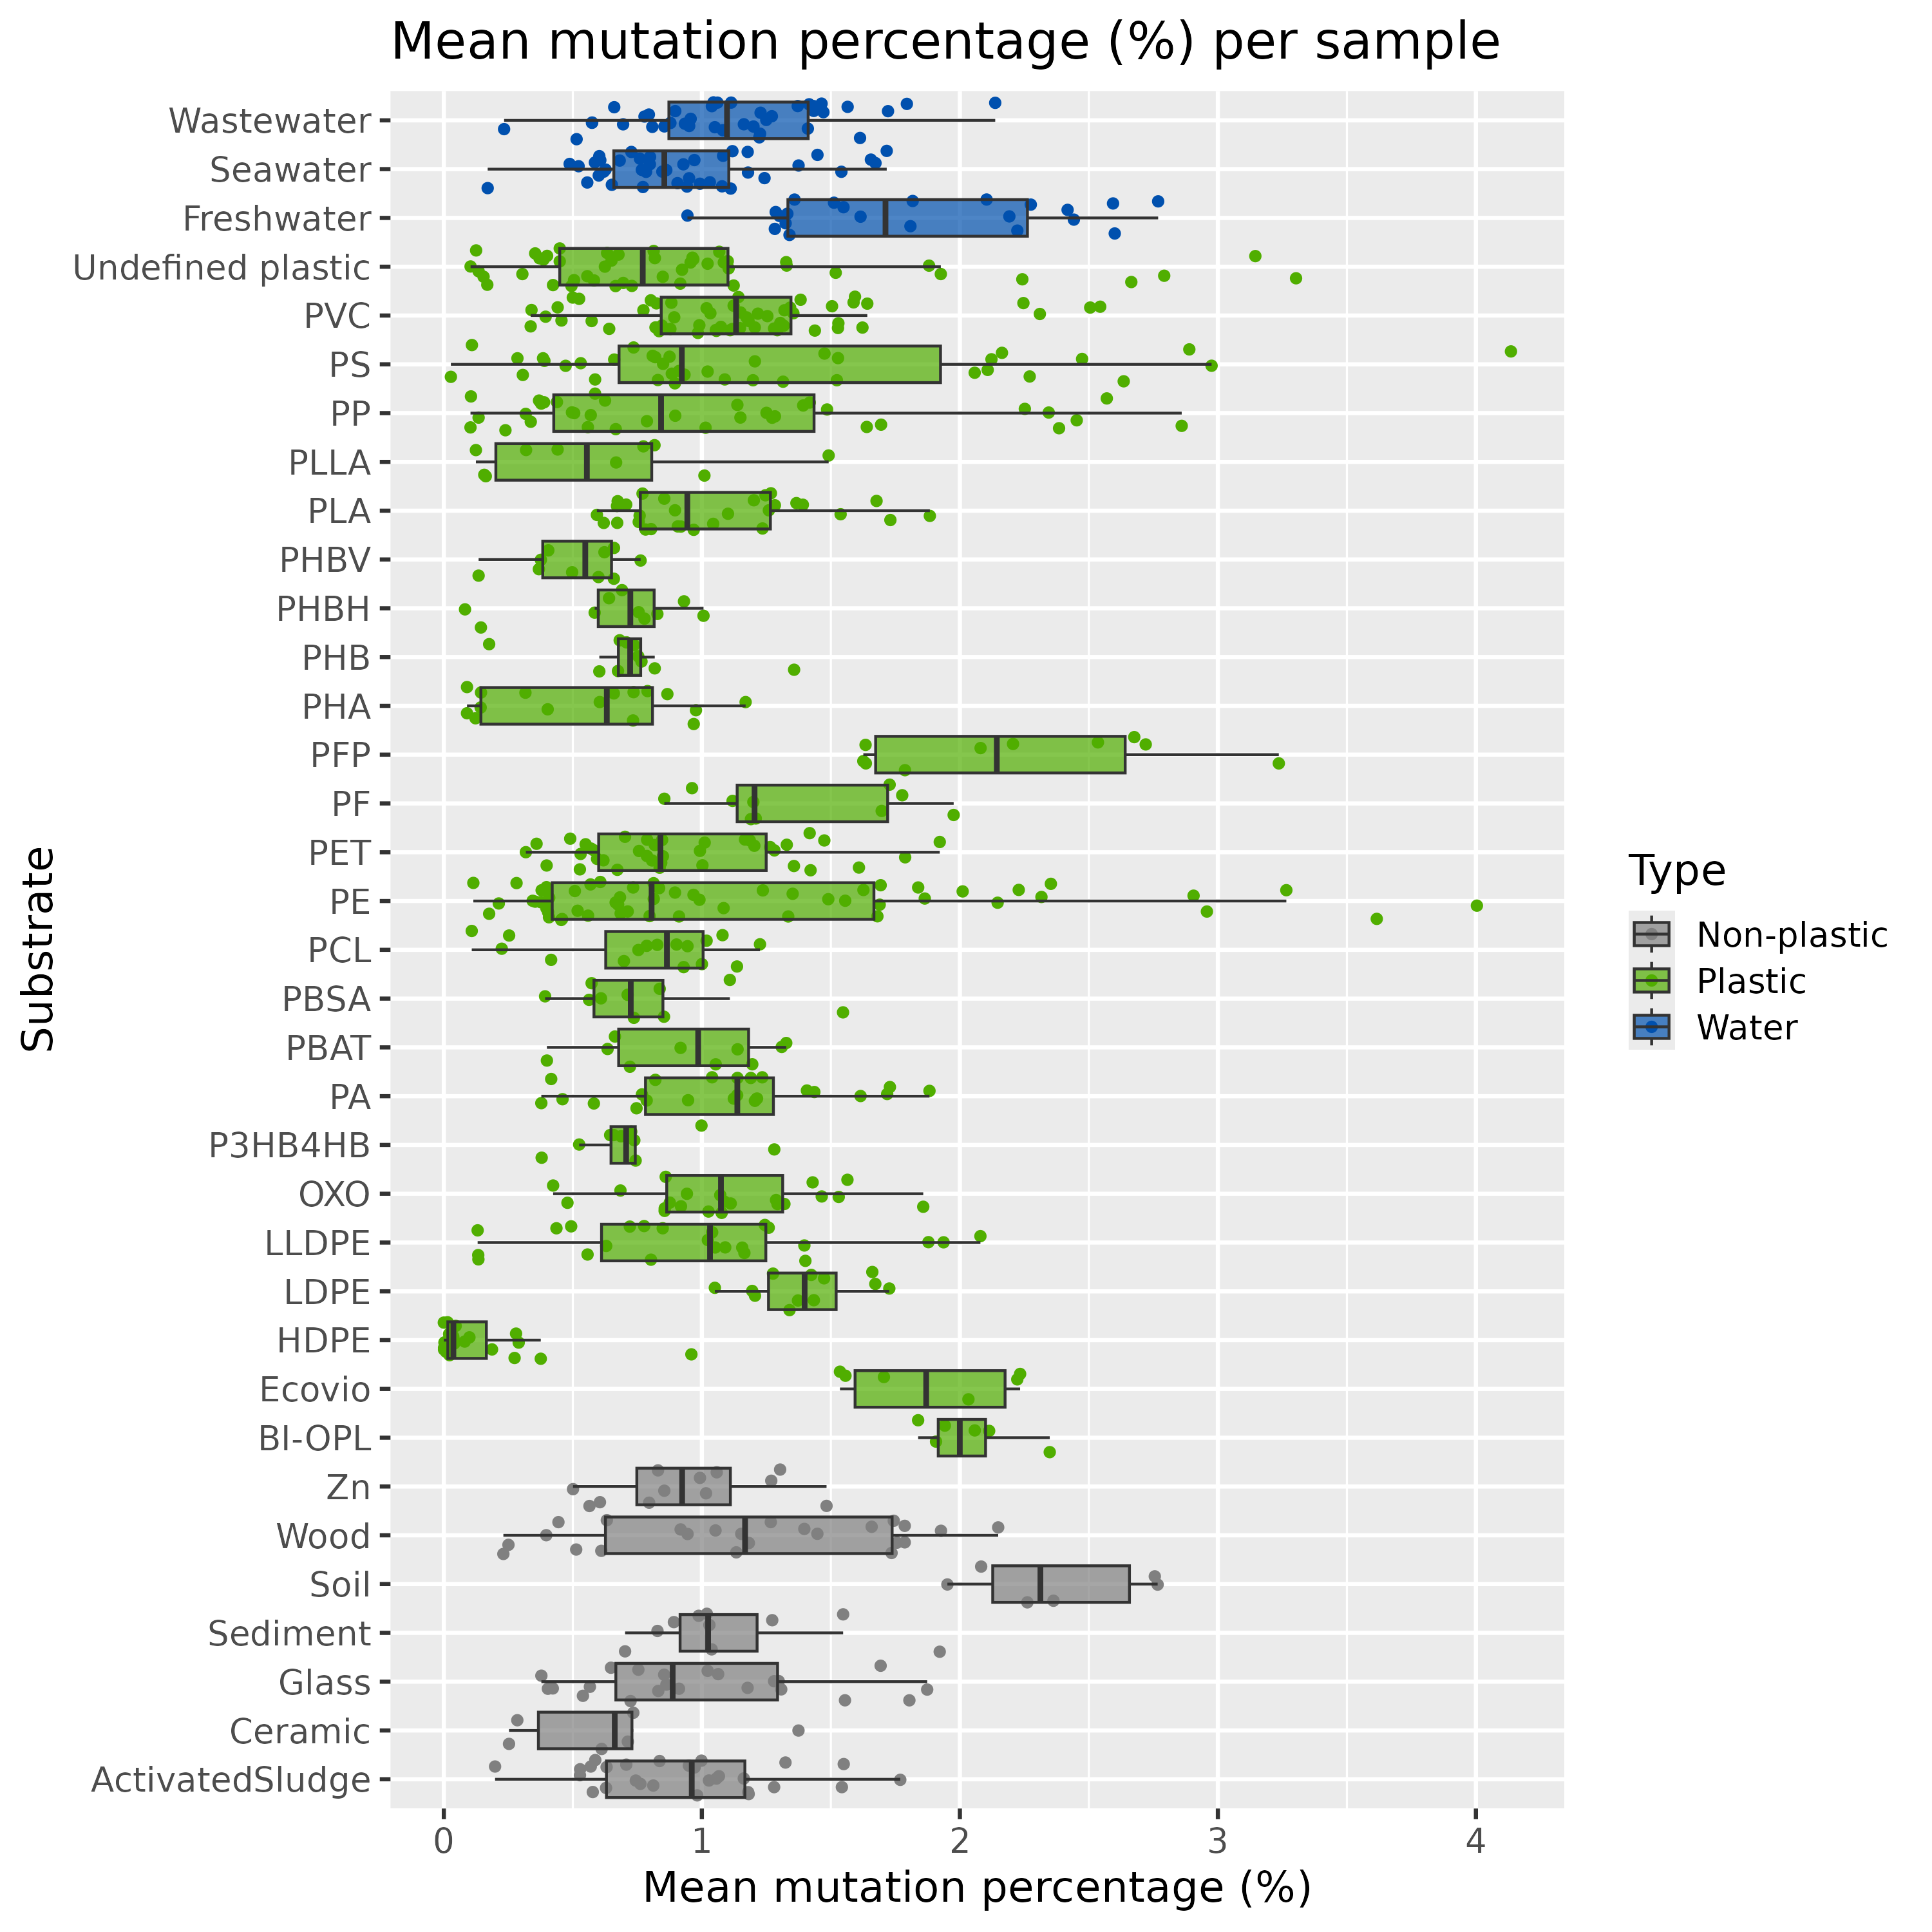
\includegraphics[width = 0.7\textwidth]{figure/mean_samples_substrate.png}
    % \caption{Mean Samples Substrate Full}
    % \label{mean_samples_substrate_full}
% \end{figure}
% 
% \begin{figure}[h]
    % \centering
    % 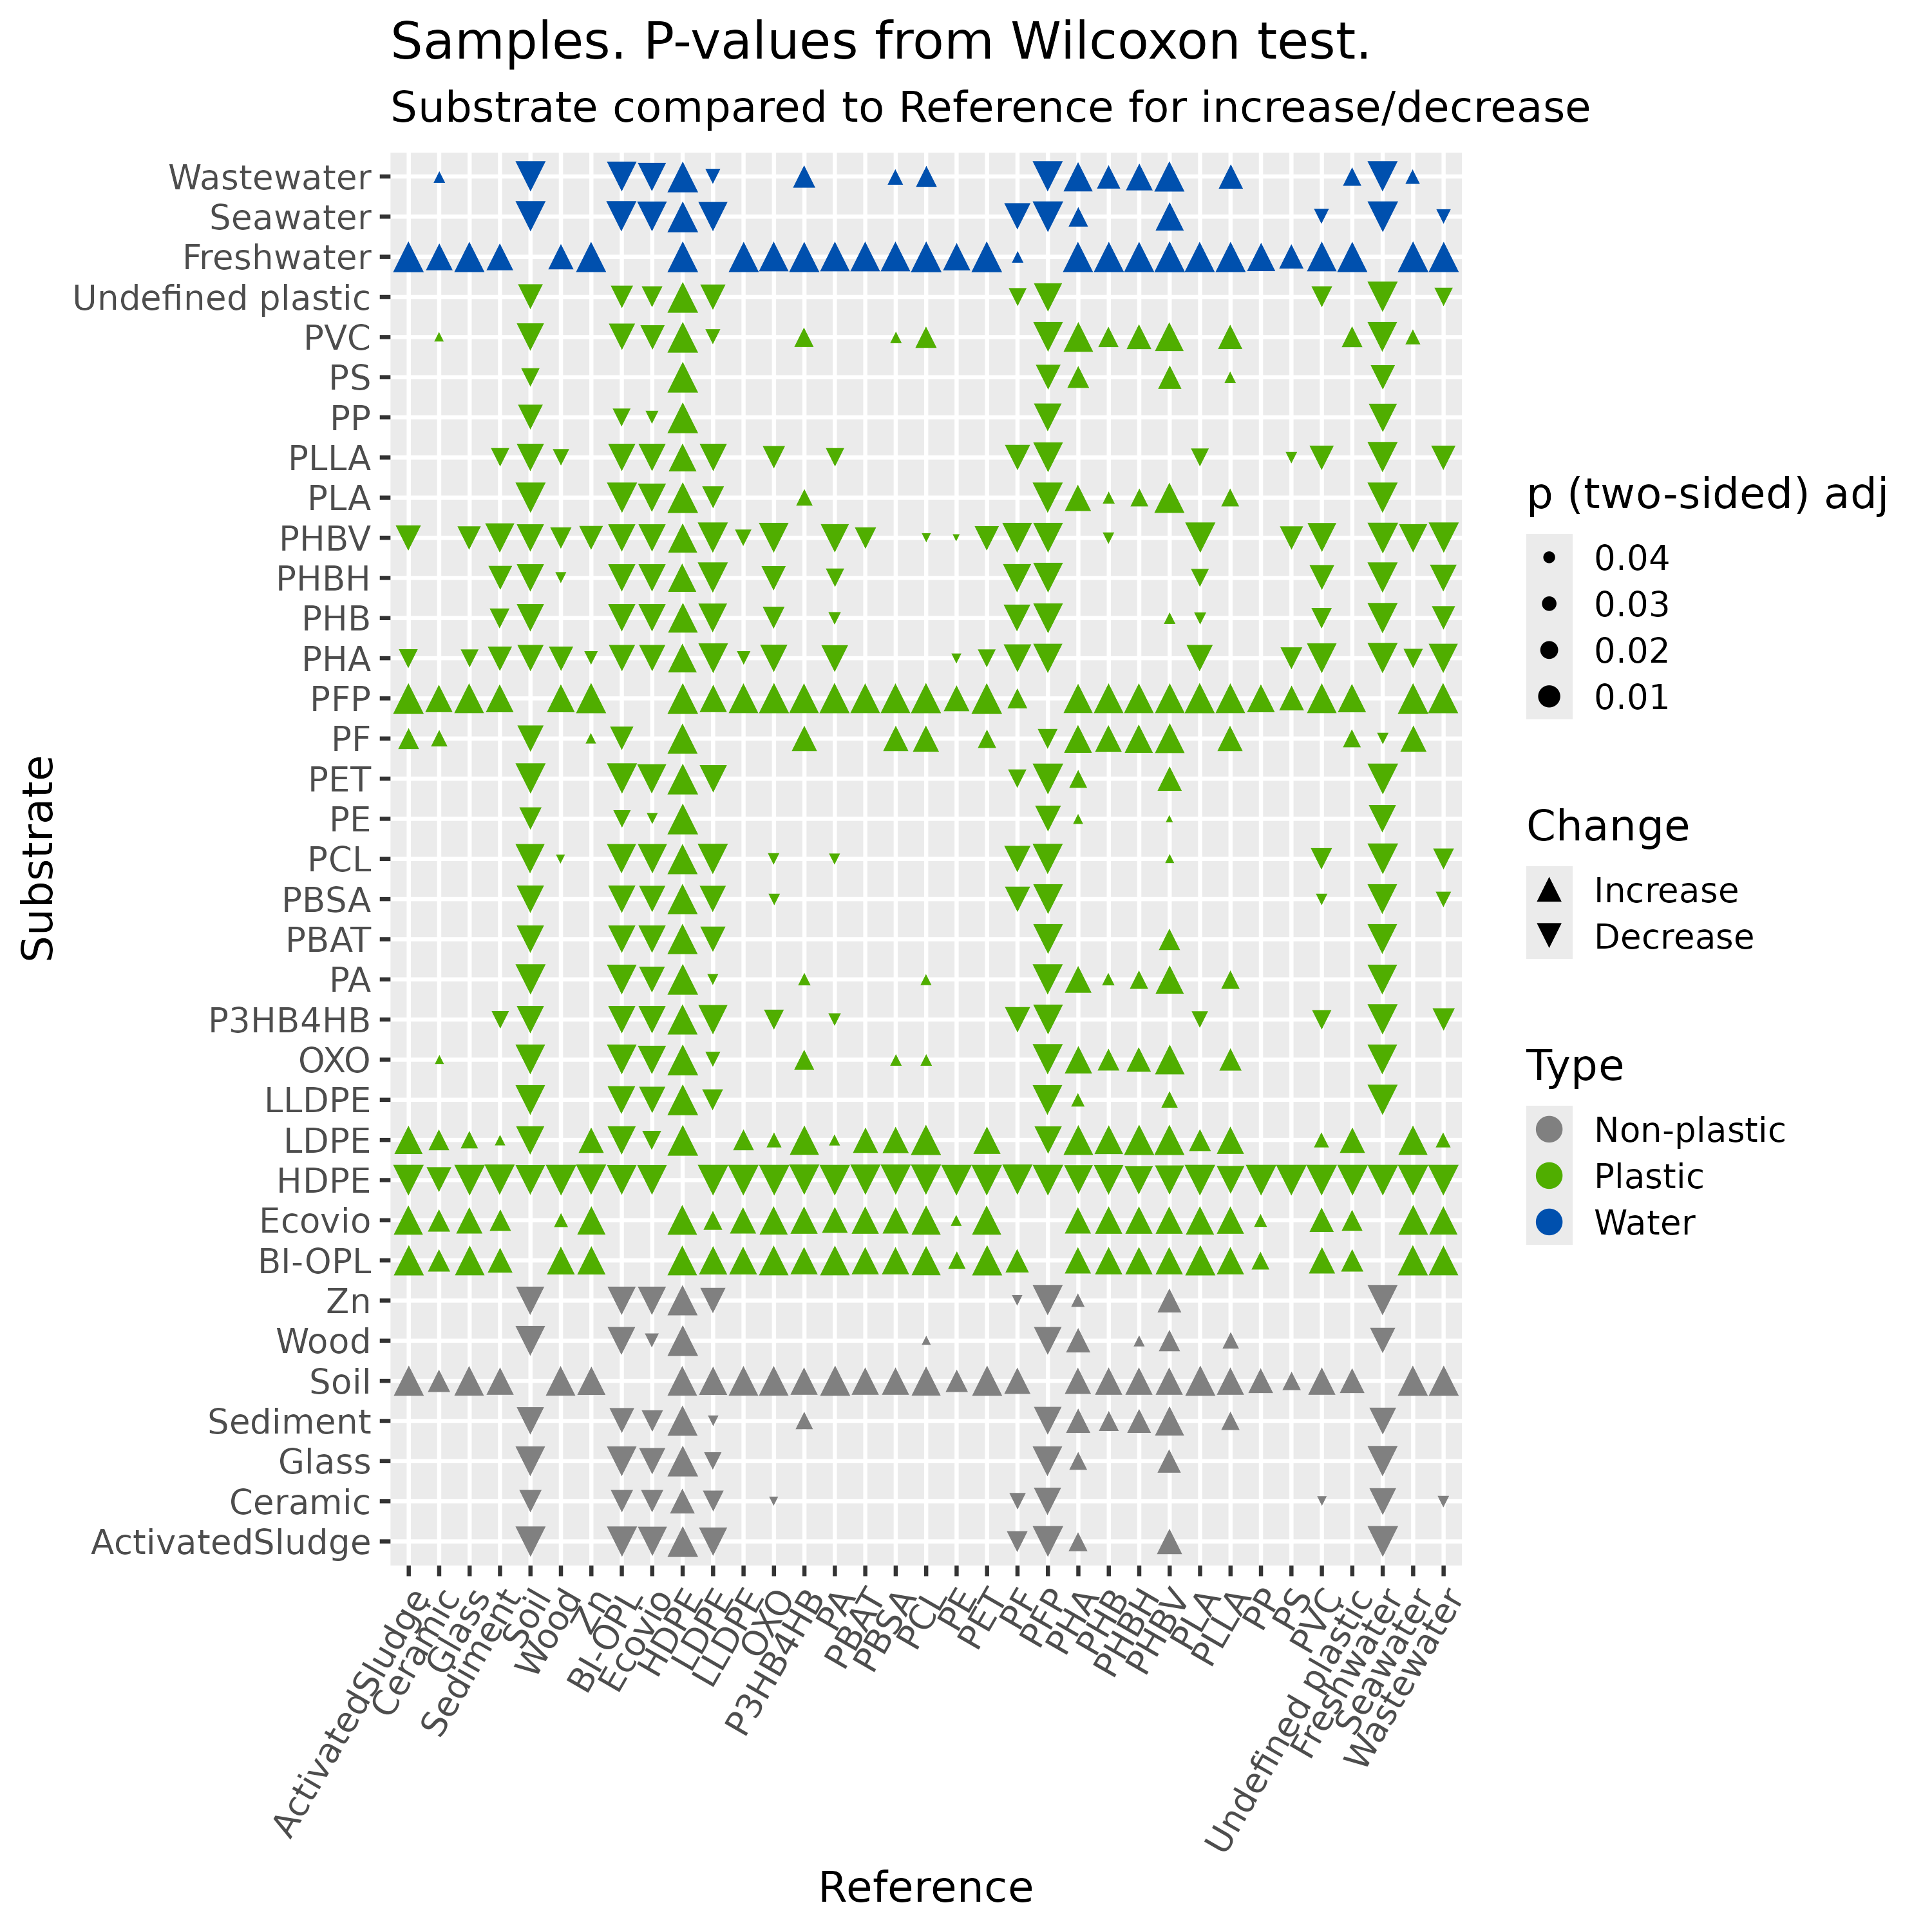
\includegraphics[width = 0.7\textwidth]{figure/wilcox_samples_substrates.png}
    % \caption{Wilcoxon Samples Substrate Full}
    % \label{wilcox_samples_substrates_full}
% \end{figure}
% 

%\subsection{Mean mutation percentage of individual mutations}
%Figure \ref{mean_genes_sampletype} show the result if instead of the mean mutation percentage for each sample was calculated, the mean mutation percentage per mutation, grouped by sampletype was calculated. \todo{i.e. mutation A12D parC for water: 10\%, A12D parC for plastic: 0\%, A12D parC for non-plastic: 3\%} 
%The resulting figure is hard to interpret since many of the genes will have a mean close to zero. If instead a log-scale was used, it removes many of the data points from the water and nonplastic groups, since they have a mean mutation percentage of zero. This skews the figure shown, and end up showing the reverse change as described below. \todo{Since we cannot use the log plot, do we need to use the bad plot instead, or can we skip it and just use stats?}
By instead looking at the mean mutation percentage of individual point mutations across samples (Figure \ref{mean_genes_sampletype}), the result was that the mean for the plastic group was significantly higher (Wilcoxon: p < 0.001) than the water group(pseudomean: +0.01). The plastic group also had a significantly higher (Wilcoxon: p < 0.001) mean mutation percentage than the non-plastic samples (pseudomean: +0.01).
There was no significant (Wilcoxon: p > 0.05) difference between the water group and the non-plastic group.

%The mean mutation percentage of the plastic samples was higher when compared to both the water samples (pseudomean: +0.00) and the non-plastic samples (pseudomean: +0.00).

%The mean mutation rate of individual point mutations grouped by sample type is shown in figure \ref{mean_genes_sampletype}. The mean mutation percentage was significantly different (p < 0.001) and higher for the plastic samples compared to both the water samples and the non-plastic samples. There was no significant difference between the water group and the non-plastic group.
% There is a significant difference between the different sample types, where plastic show an increase compared to both the water samples and the non-plastic samples.

\begin{figure}[h!]
    \centering
    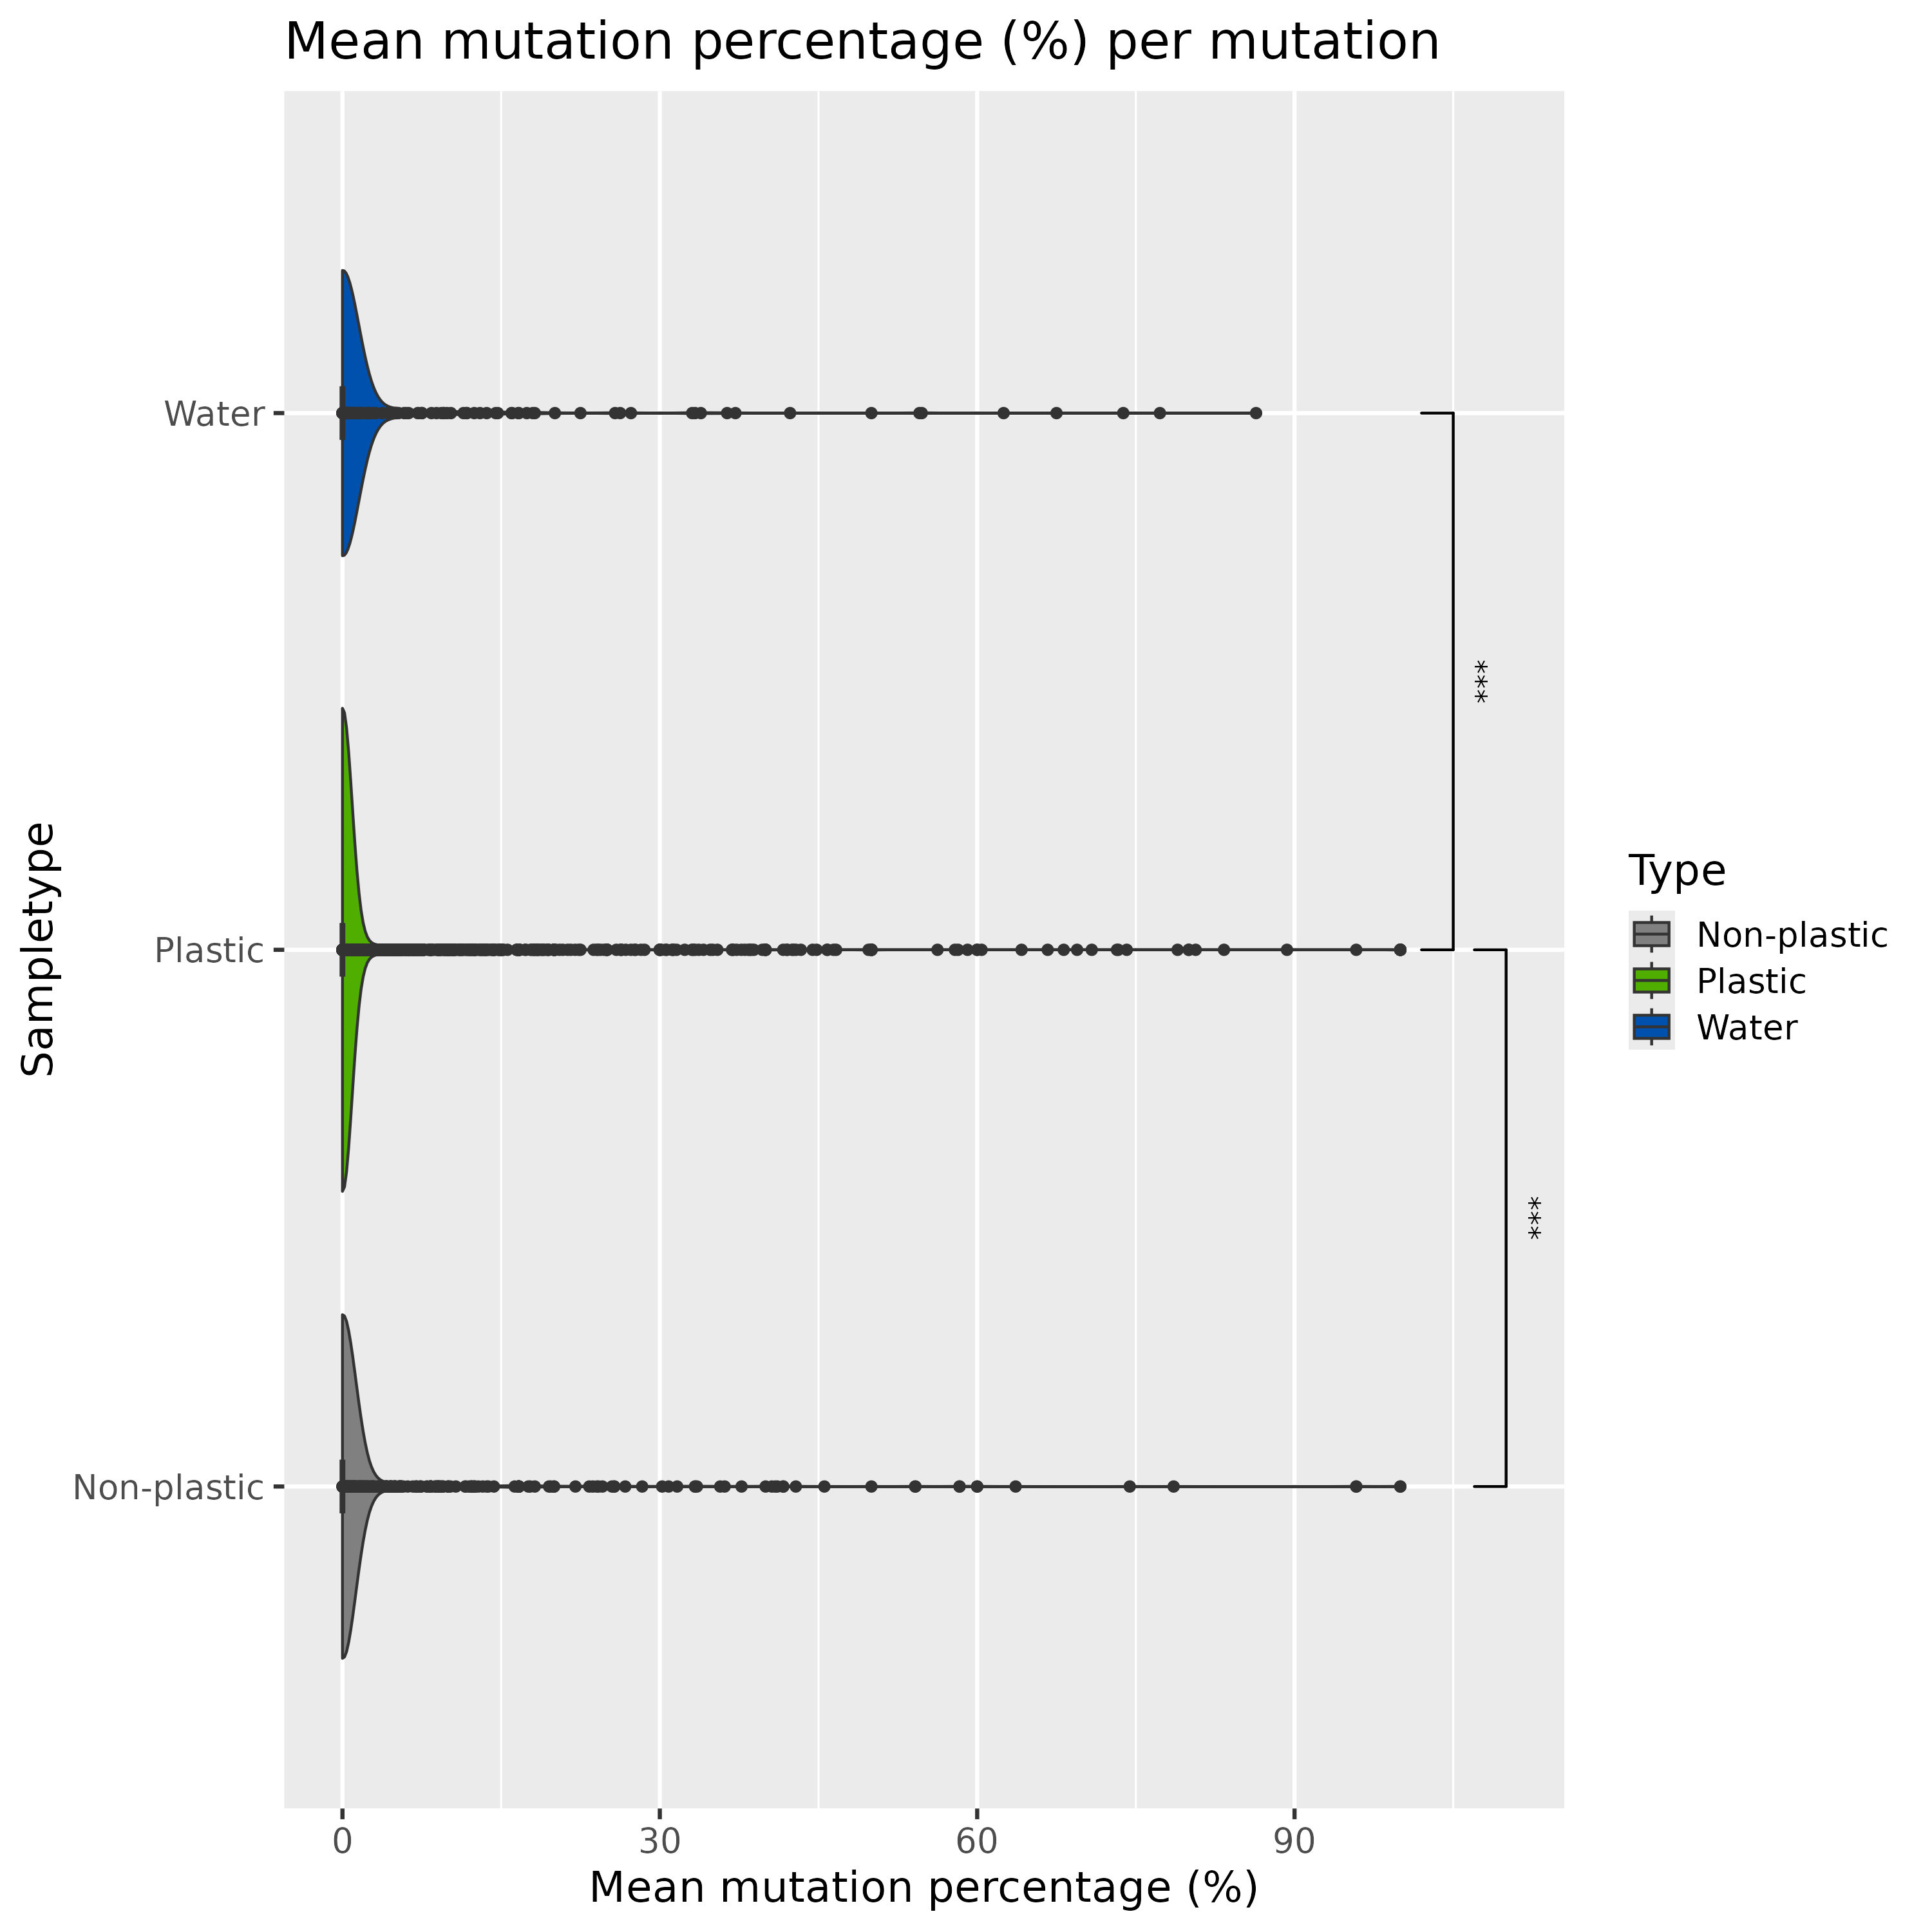
\includegraphics[width = 0.7\textwidth]{figure/mean_genes_sampletype.png}
    \caption{Mean mutation percentage (\%) per sample, grouped by sampletype. *** = p < 0.001}
    \label{mean_genes_sampletype}
\end{figure}

There were numerous differences between the different substrates when the mean mutation percentage per mutation was compared between substrates (Figure \ref{mean_genes_substrate}). This is supported by Figure \ref{wilcox_genes_substrate} which show the p-values from a Wilcoxon test between the different substrates.
% Since figure \ref{mean_genes_substrate} uses a log-scale for visibility, the normal interpretation of the box-plot cannot be done since many points are erroneously removed, and therefore is only for visualizing the mutation rate.
The substrates which had the highest mean mutation percentage were PFP, PE, Ecovio, and BI-OPL from the plastic group as well as soil and wood from the non-plastic sampletypes. 
Freshwater had a significant increase of mean mutation percentage compared to most other substrates.

% FROM samples substrates: 
% In figure \ref{mean_samples_substrate} the samples are instead grouped by substrate type, which show that there are differences for different plastics, as well as other substrates. Figure \ref{wilcox_samples_substrate} show the statistical significance of the comparison, when a wilcoxon test was done for the Substrate versus the Reference, as well as if there is an increase of the pseudo-mean compared to the reference. Note that all comparisons were done, but only the significant ones (p < 0.05) are shown. It is shown that there are some plastics that has a significant higher mean mutation percentage than most other substrates. These include PFP, LDPE, Ecovio and BI-OPL. The last two plastics are biodegradable plastics. The plastic substrates that has a significant higher mean mutation percentage than seawater or wastewater include PVC and PF in addition to the other plastics mentioned before. There are also some plastics which have significantly different lower mean mutation percentage than almost all other substrates, the most notable of which is high-density polyethylene (HDPE), poly(3-hydroxybutyrate-co-3-hydroxyvalerate) (PHBV) and polyhydroxyalkanoate (PHA), of which the latter two are biodegradable polymers while the first one is not. Almost all substrates has a significantly different lower mean mutation percentage than the freshwater samples, the exception of which is leaf, rock, Ecovio, BI-OPL, and PFP where there is no significant difference. The soil samples also has a significant higher mean mutation percentage compared to many other substrates.

\begin{figure}[h!]
    \centering
    \subfloat[\label{mean_genes_substrate}]{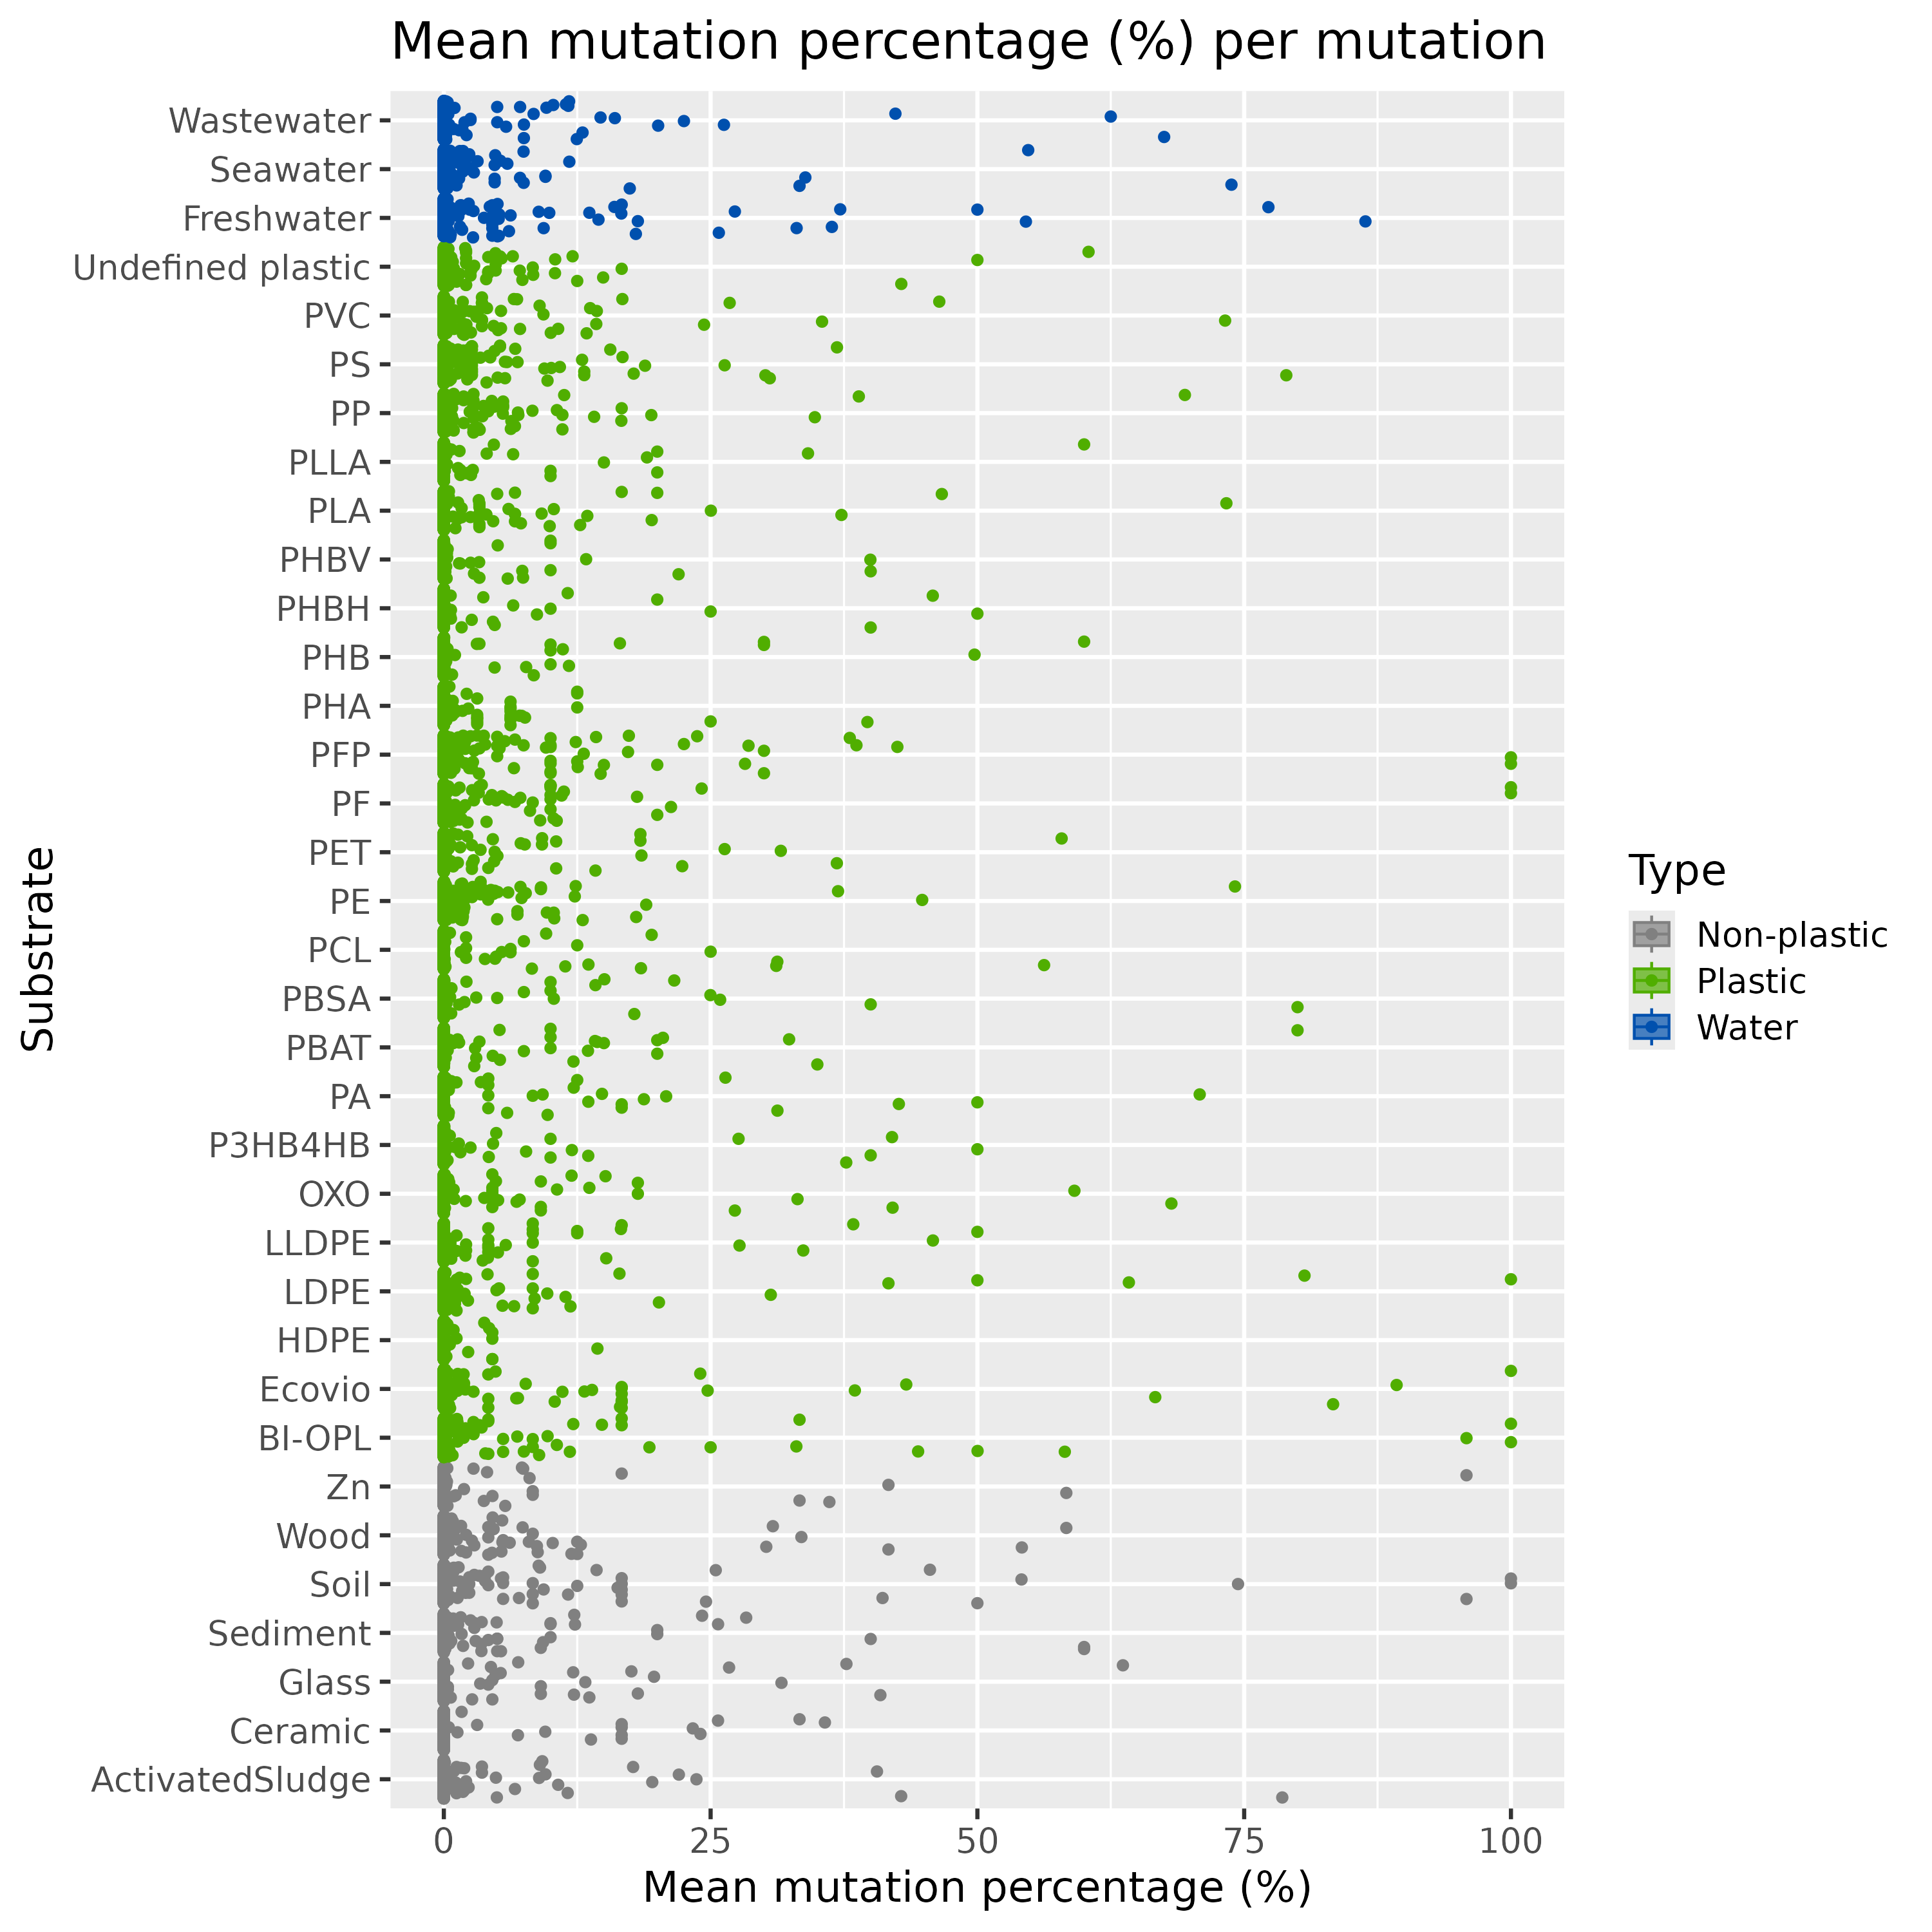
\includegraphics[width=0.5\textwidth]{figure/mean_genes_substrate.png}} 
    \subfloat[\label{wilcox_genes_substrate}]{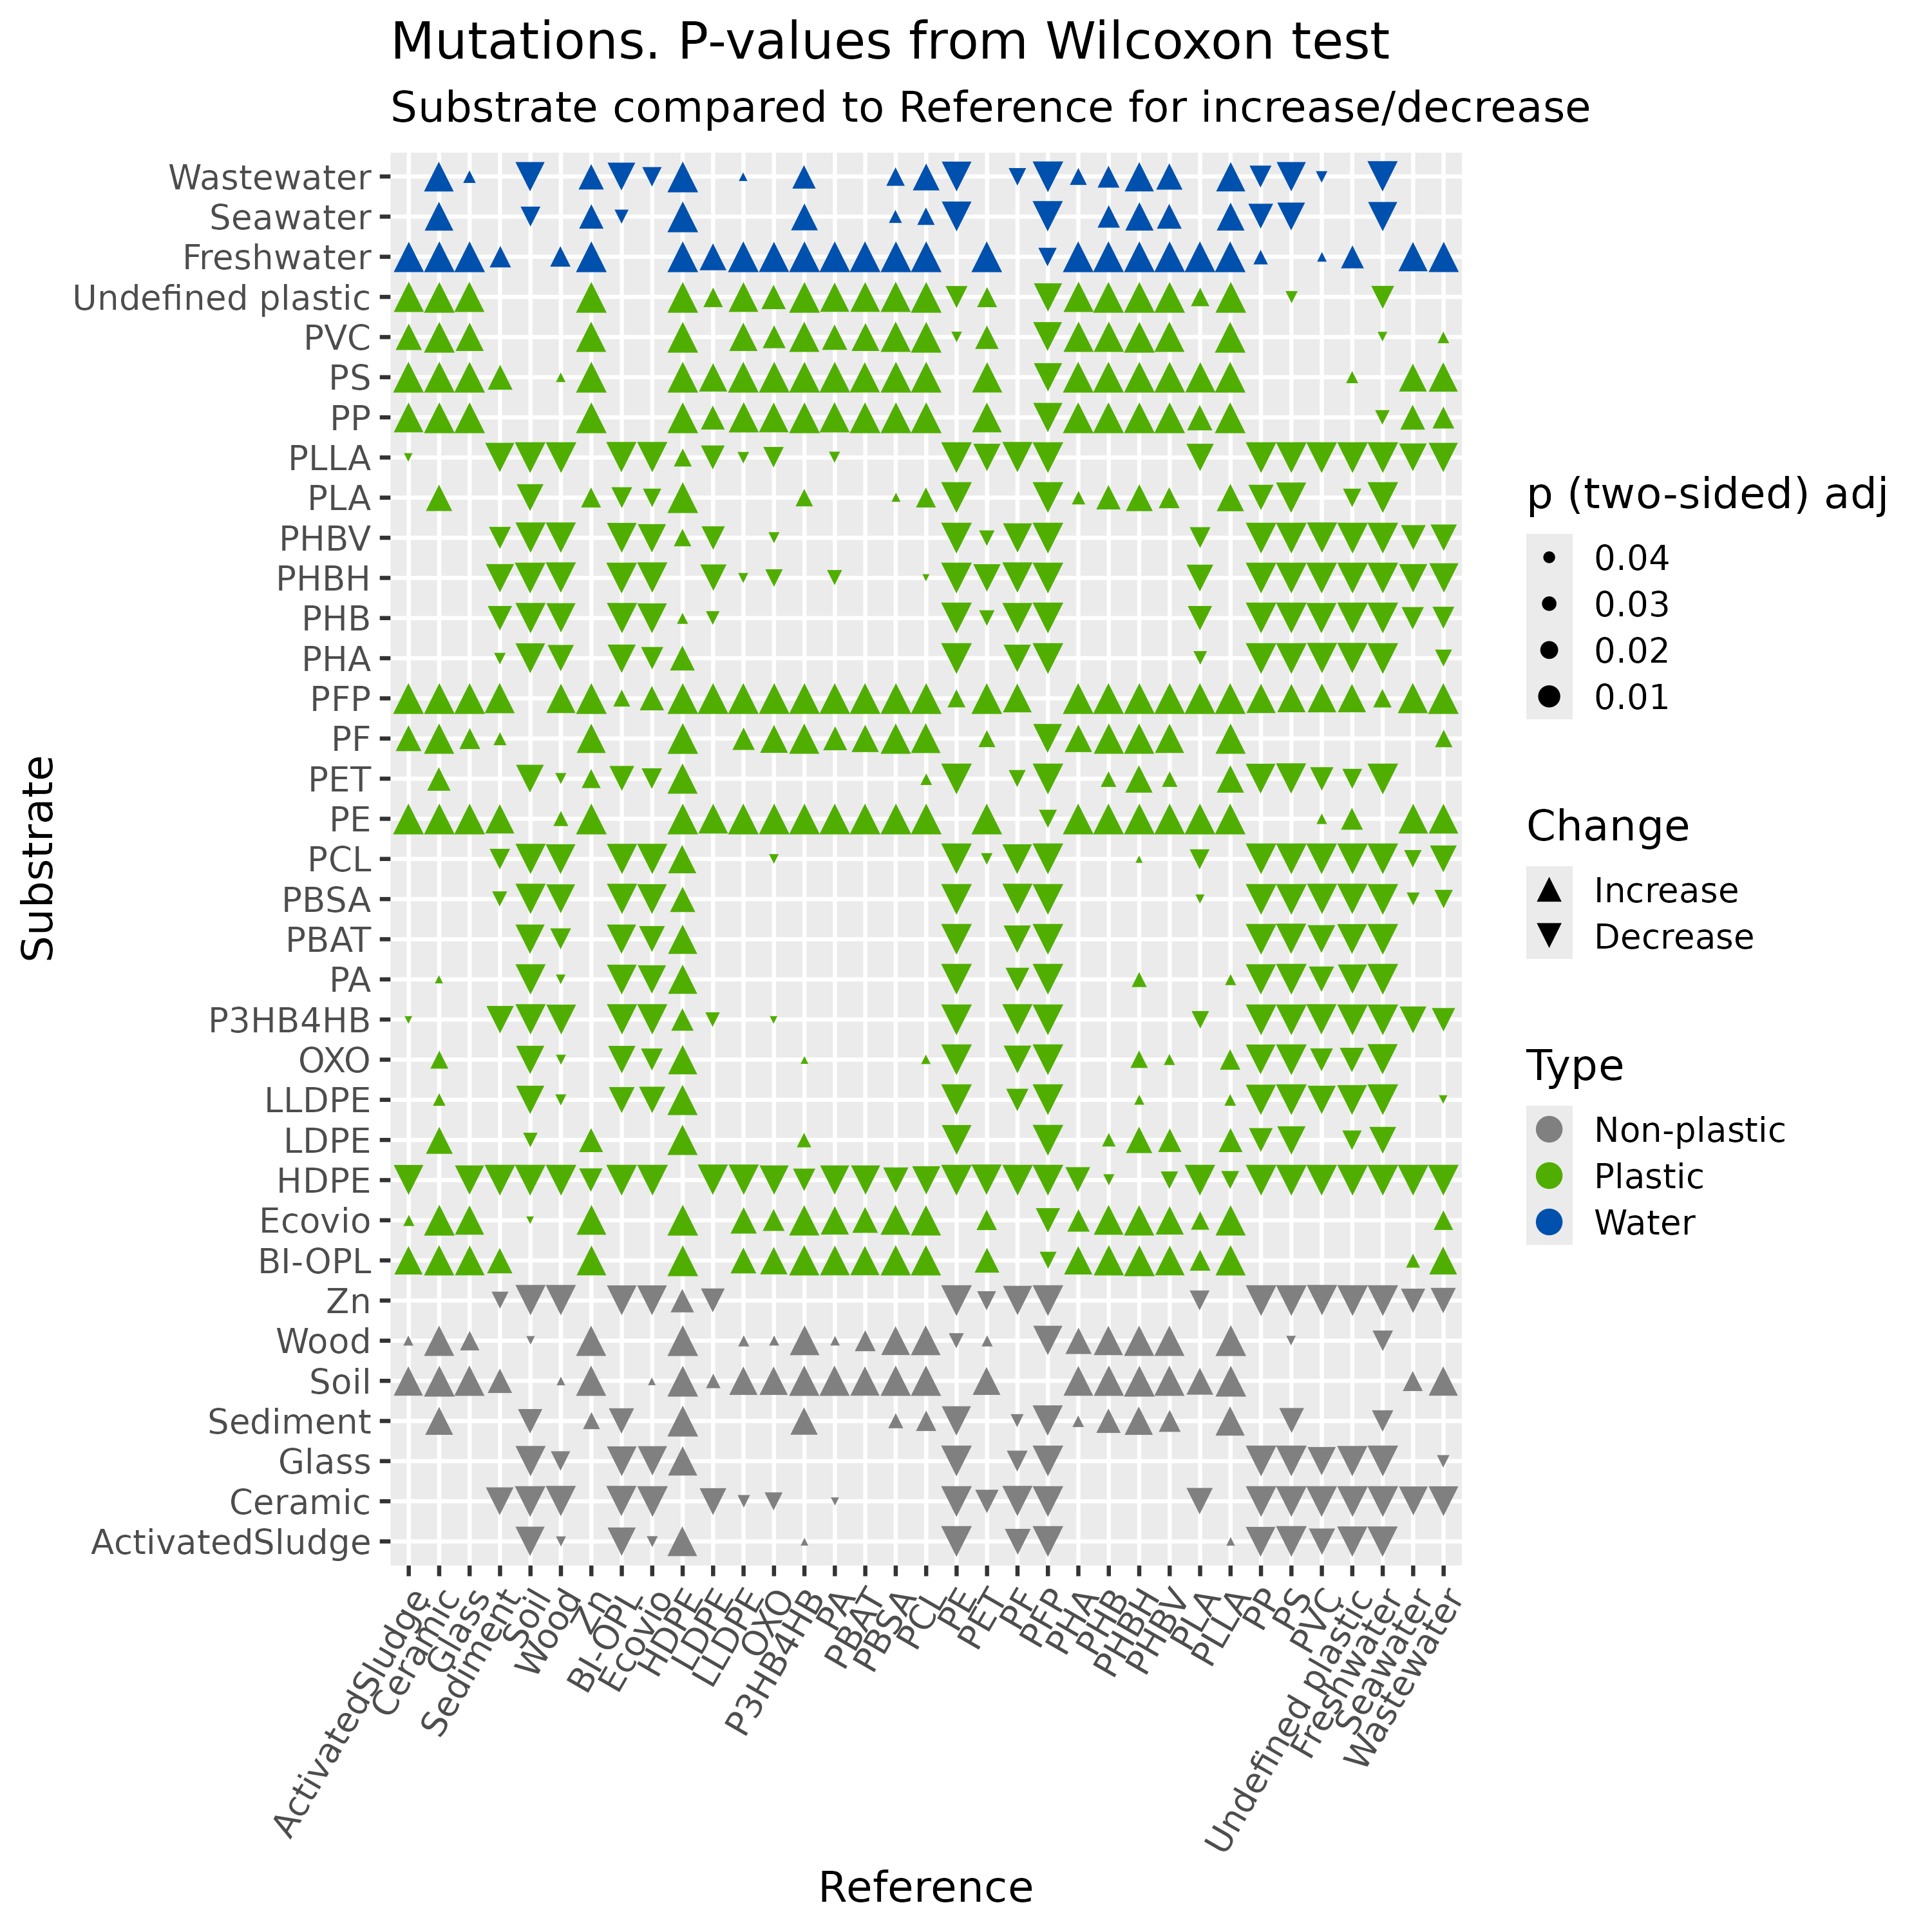
\includegraphics[width=0.5\textwidth]{figure/wilcox_genes_substrates.png}}
    \caption{(a) Mean mutation percentage per mutation, grouped by substrate type. (b) p-values from Wilcoxon test of mean mutation percentage for Substrate versus Reference}
    \label{both_mean_genes_substrate}
\end{figure}

When we subset the mean mutation percentage to only the point mutations which had a mean mutation rate of at least 25 percent in any substrate, it is evident
%Figure \ref{pointplot_mutations} show the mean mutation percentage for point mutations with a mean mutation percentage higher than 25 percent in any substrate. 
that there were certain mutations which occured in most substrates, and several that only occured in some substrates. The ones which occured in almost all samples were Q1073R in rpoB which confer resistance to rifampicin, G1245B in gyrB which confer resistance to aminocoumarin, and D244Y in rpoC which confer resistance to vancomycin.
%\todo{Mention Ecovio, BI-OPL, PFP, Freshwater, Soil with many point mutations of high mean mutation percentage?}

\begin{figure}[!h]
    \centering
    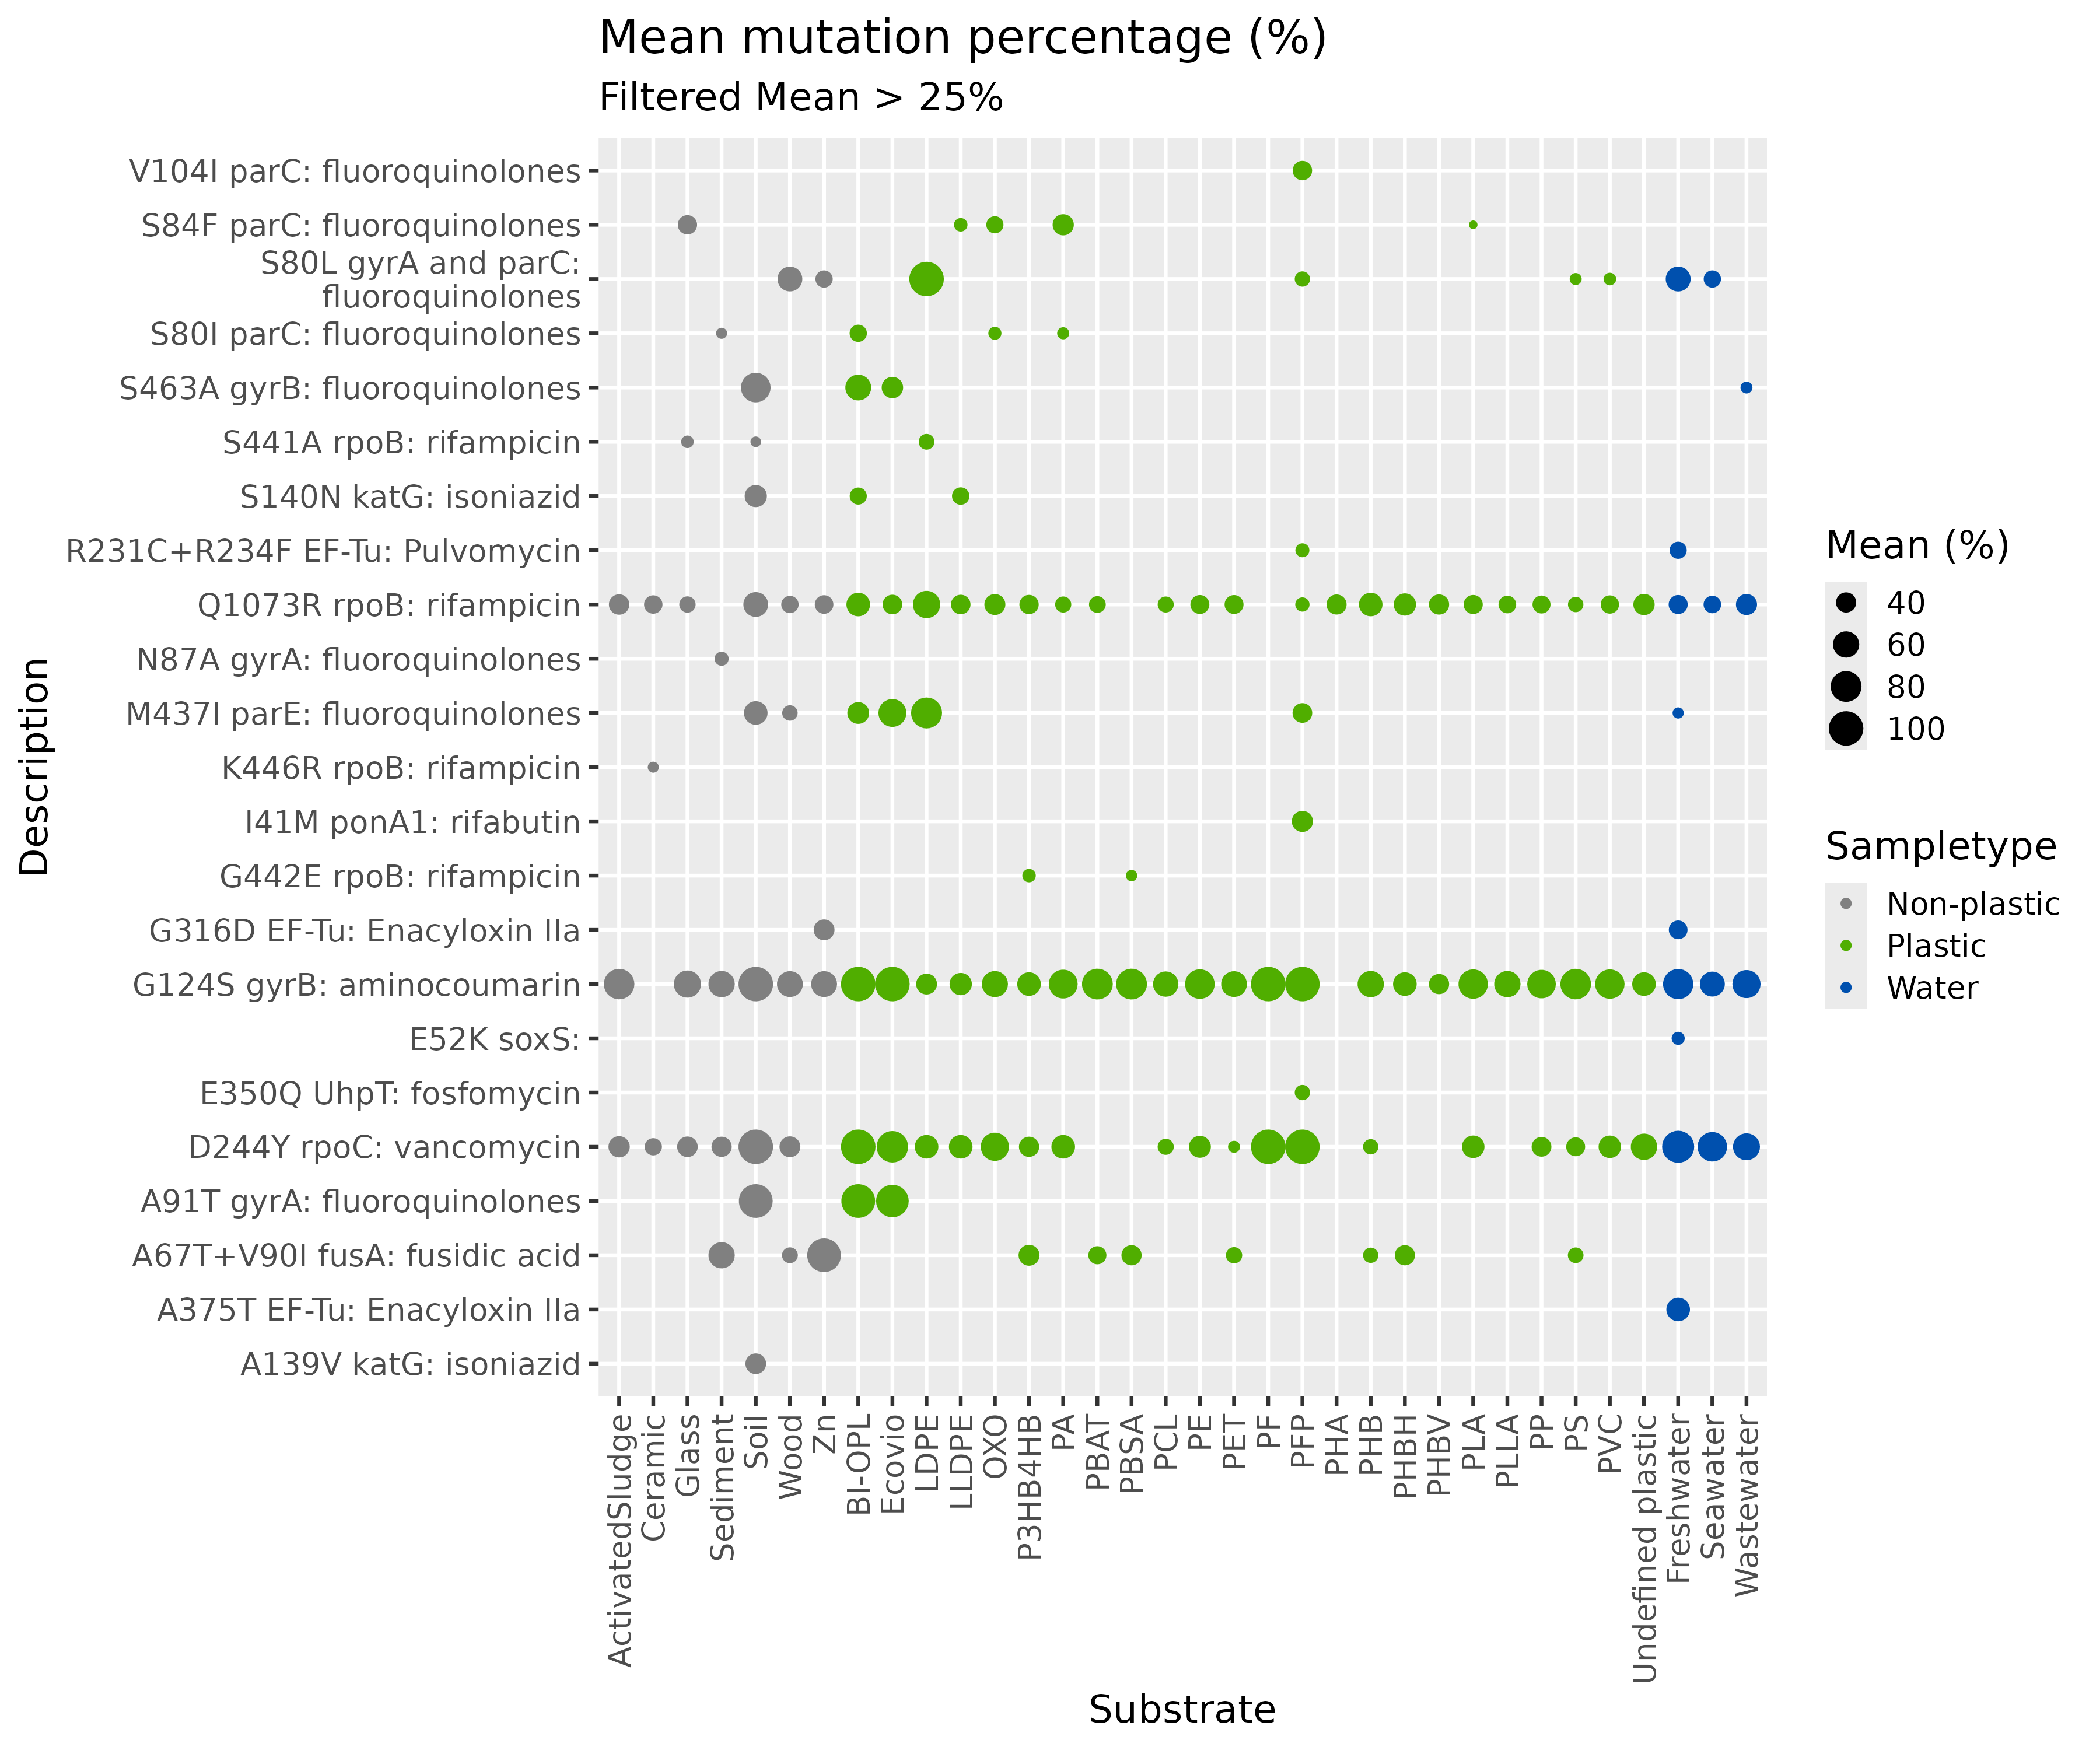
\includegraphics[width = \textwidth]{figure/relative_mean_points_25.png}
    \caption{Filtered mean mutation percentage per mutation.}
    \label{pointplot_mutations}
\end{figure}


\section{Predicting substrate identifiers} 
% Rename to something else, "Predicting sample  
% Removed:
% D87H:Pseudomonas aeruginosa gyrA: fluoroquinolones
% D87H:Burkholderia dolosa gyrA: fluoroquinolones
%
% Renamed: There is one AMR Gene Family which has a very long name:
% "ATP-binding cassette (ABC) antibiotic efflux pump;General Bacterial Porin with reduced permeability to beta-lactams;major facilitator superfamily (MFS) antibiotic efflux pump;resistance-nodulation-cell division (RND) antibiotic efflux pump"
In the following figures only the top ten genes and gene families which serves as significant predictors for substrates are shown.
%In the following figures only the ten most significant AMR Gene Families or mutations are shown. 
%However, there are in all cases several more which are not shown. 
%Figures showing all the 50 most significant variables can be found in Appendix \ref{appendix:code}.
%\todo{Do this? Not sure if \emph{all} of them can be shown, but at least 50 is possible in a really long plot}

\subsection{AMR Gene Family}
In the database CARD, each mutation is associated with an AMR Gene Family, which is a classification tag such as "rifampicin resistant rpoC" or "fluoroquinolone resistant parC". The AMR Gene Family is used in this analysis since it enables us to group the mutations by gene and conferred antibiotic resistance.
%in order to identify the function of the mutations present in the samples.

%\subsubsection{Sampletypes}
Based on the mean decrease in Gini impurity, certain AMR Gene families were significantly (p < 0.001) assigned to the non-plastic sampletype, as shown in Figure \ref{amr_sampletype}. These included fluoroquinolone resistant parC and gyrA as well as daptomycin-resistant beta-subunit of RNA polymerase (rpoB). 
%Figure \ref{amr_sampletype_bar} show the mean decrease in Gini impurity for five different AMR Gene Families, which was found to be significant.
%{true or not? true since kruskal-wallace test found X taxa singificant} when the samples are grouped by sampletype.
%Three of the families may be used to identify the non-plastic samples, which include fluoroquinolone resistant parC and gyrA as well as daptomycin-resistant beta-subunit of RNA polymerase (rpoB). 
The two significant AMR Gene Families for the water samples were vancomycin-resistant beta prime subunit of RNA polymerase (rpoC) and rifampicin-reistant rpoC. 
However, note the negative sign of these which indicate that these AMR Gene Families were more important to determine that a sample was in the reference group (the other groups) than in the water group. 
%\{It is significant, shows that a samples is NOT in the water group. As mentioned above. Can only say that a sample is from the non-plastic group, or NOT in the water group, not the abundance of it.}

\begin{figure}[h]
    \centering
    \subfloat[\label{amr_sampletype_bar}]{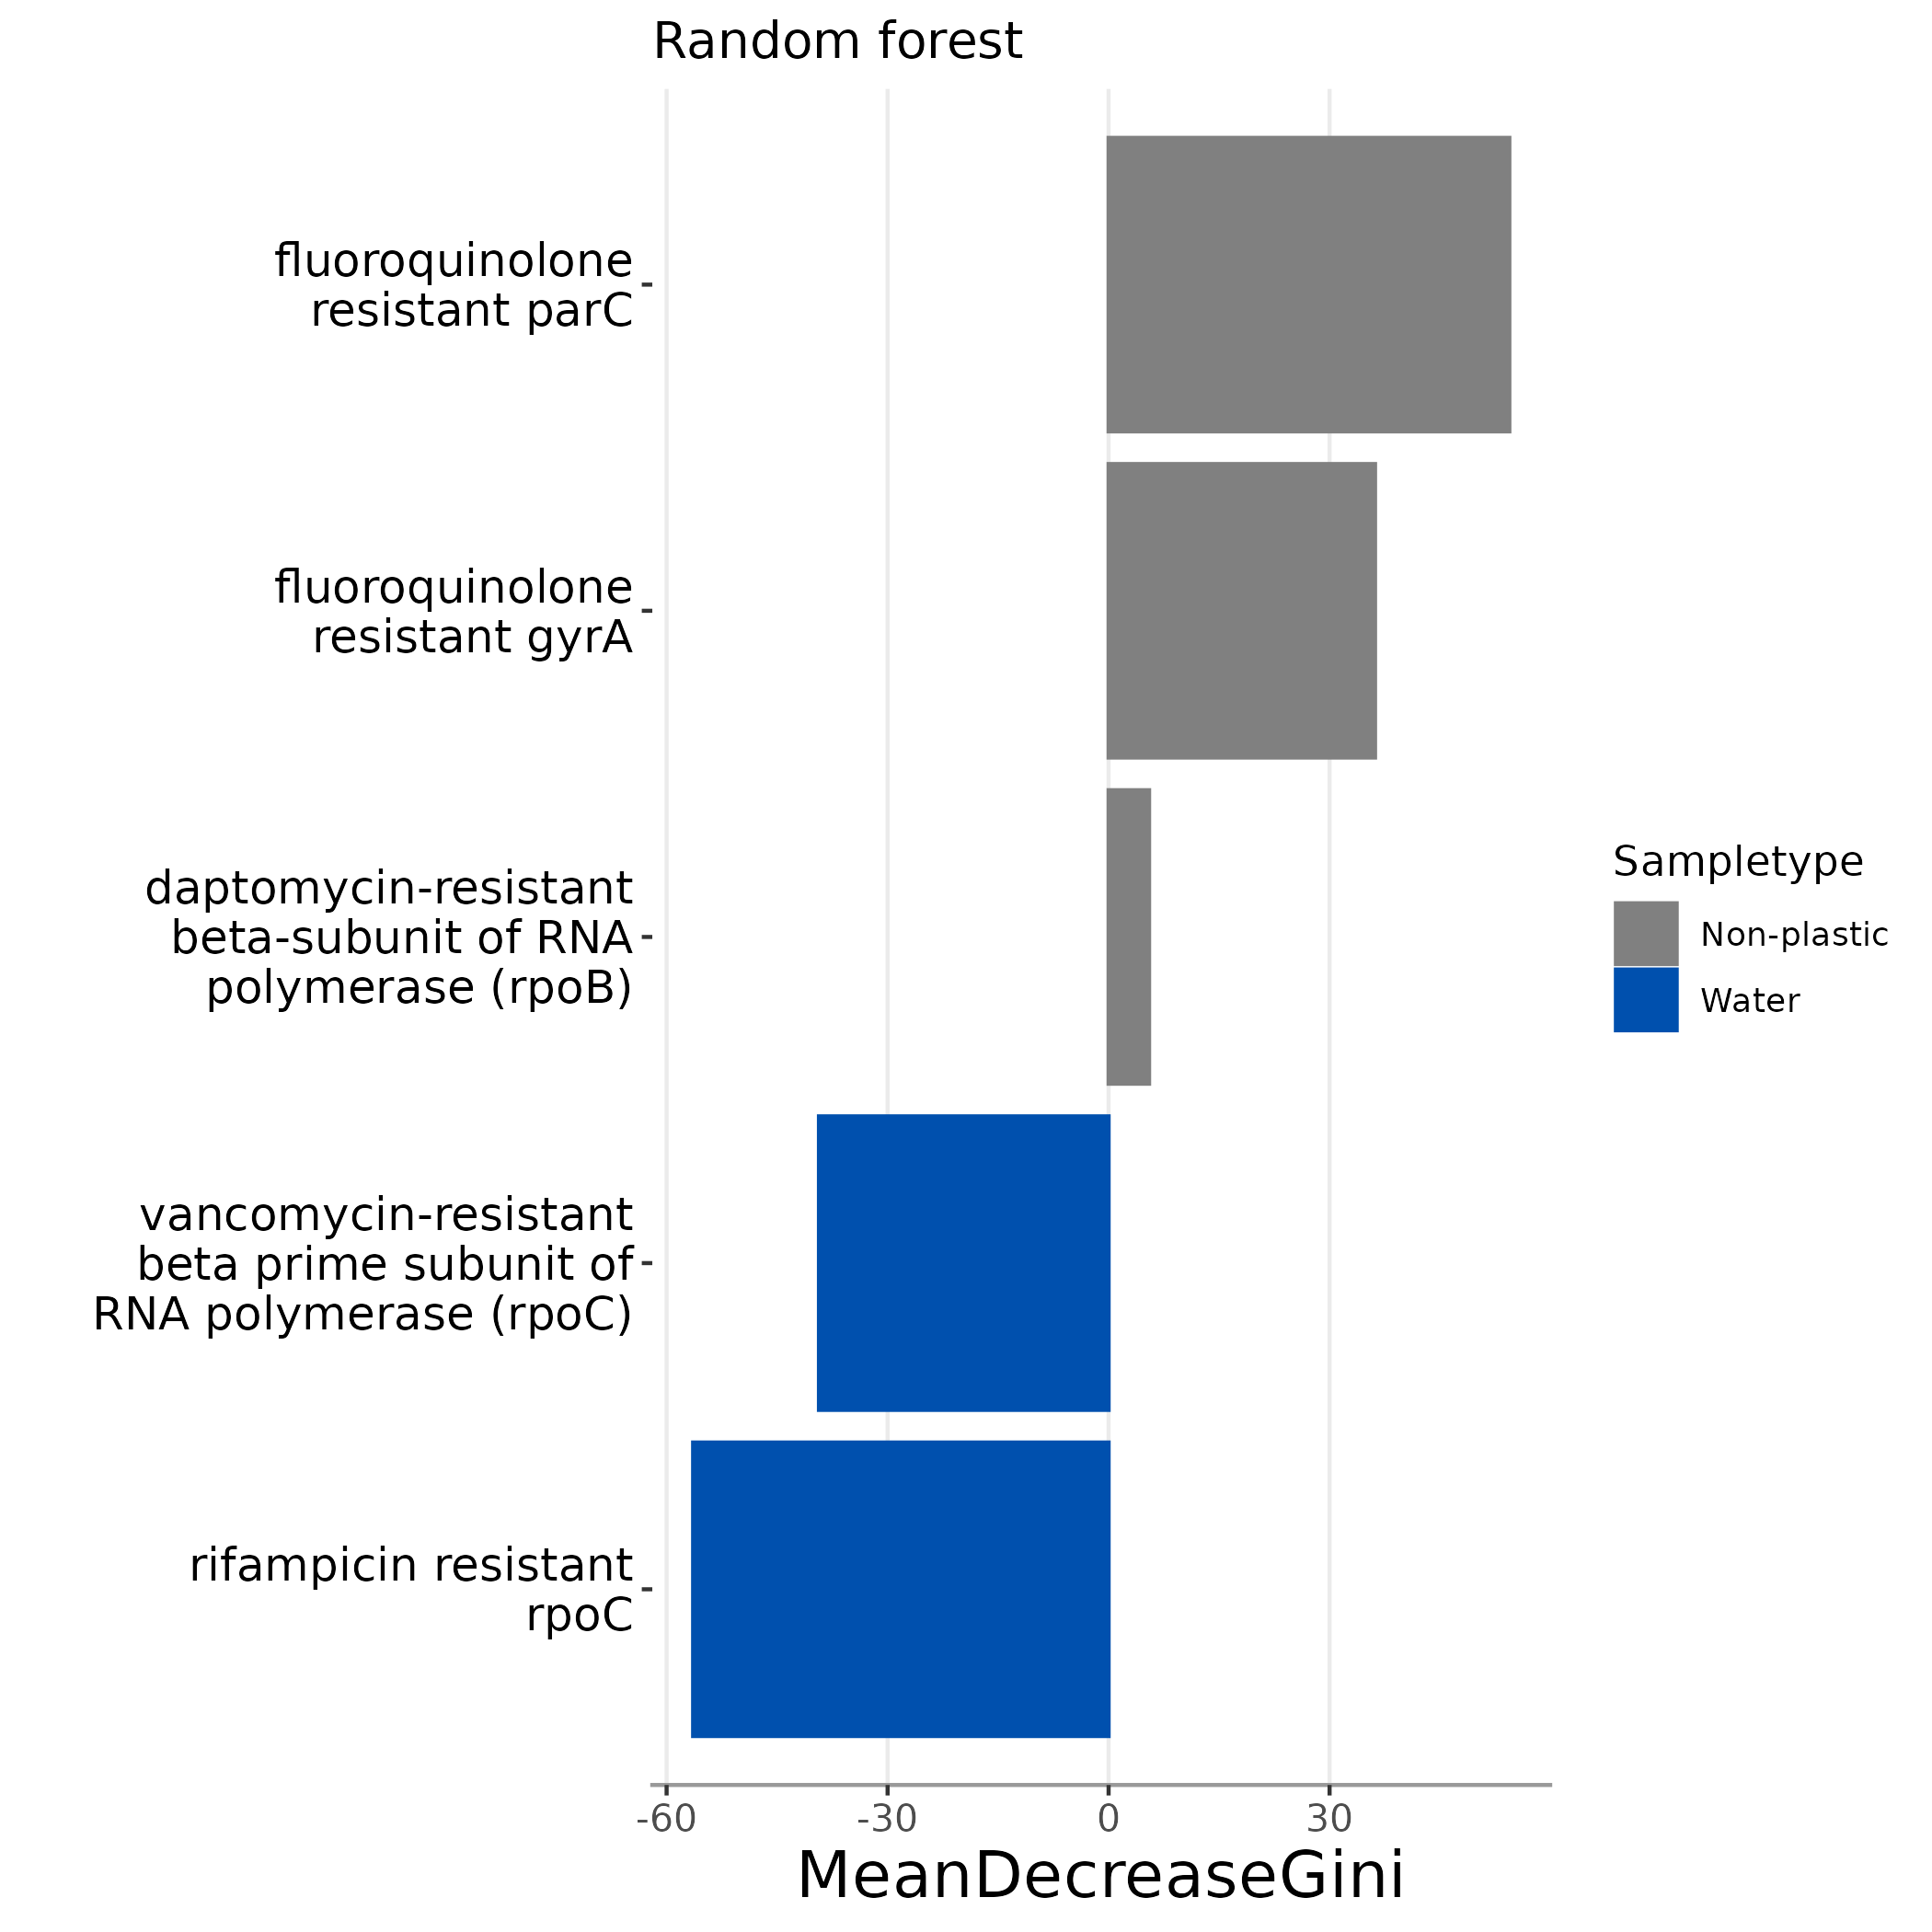
\includegraphics[width=0.5\textwidth]{figure/relative_forest_sampletype_amr_bar.png}}
    \subfloat[\label{amr_sampletype_abund}]{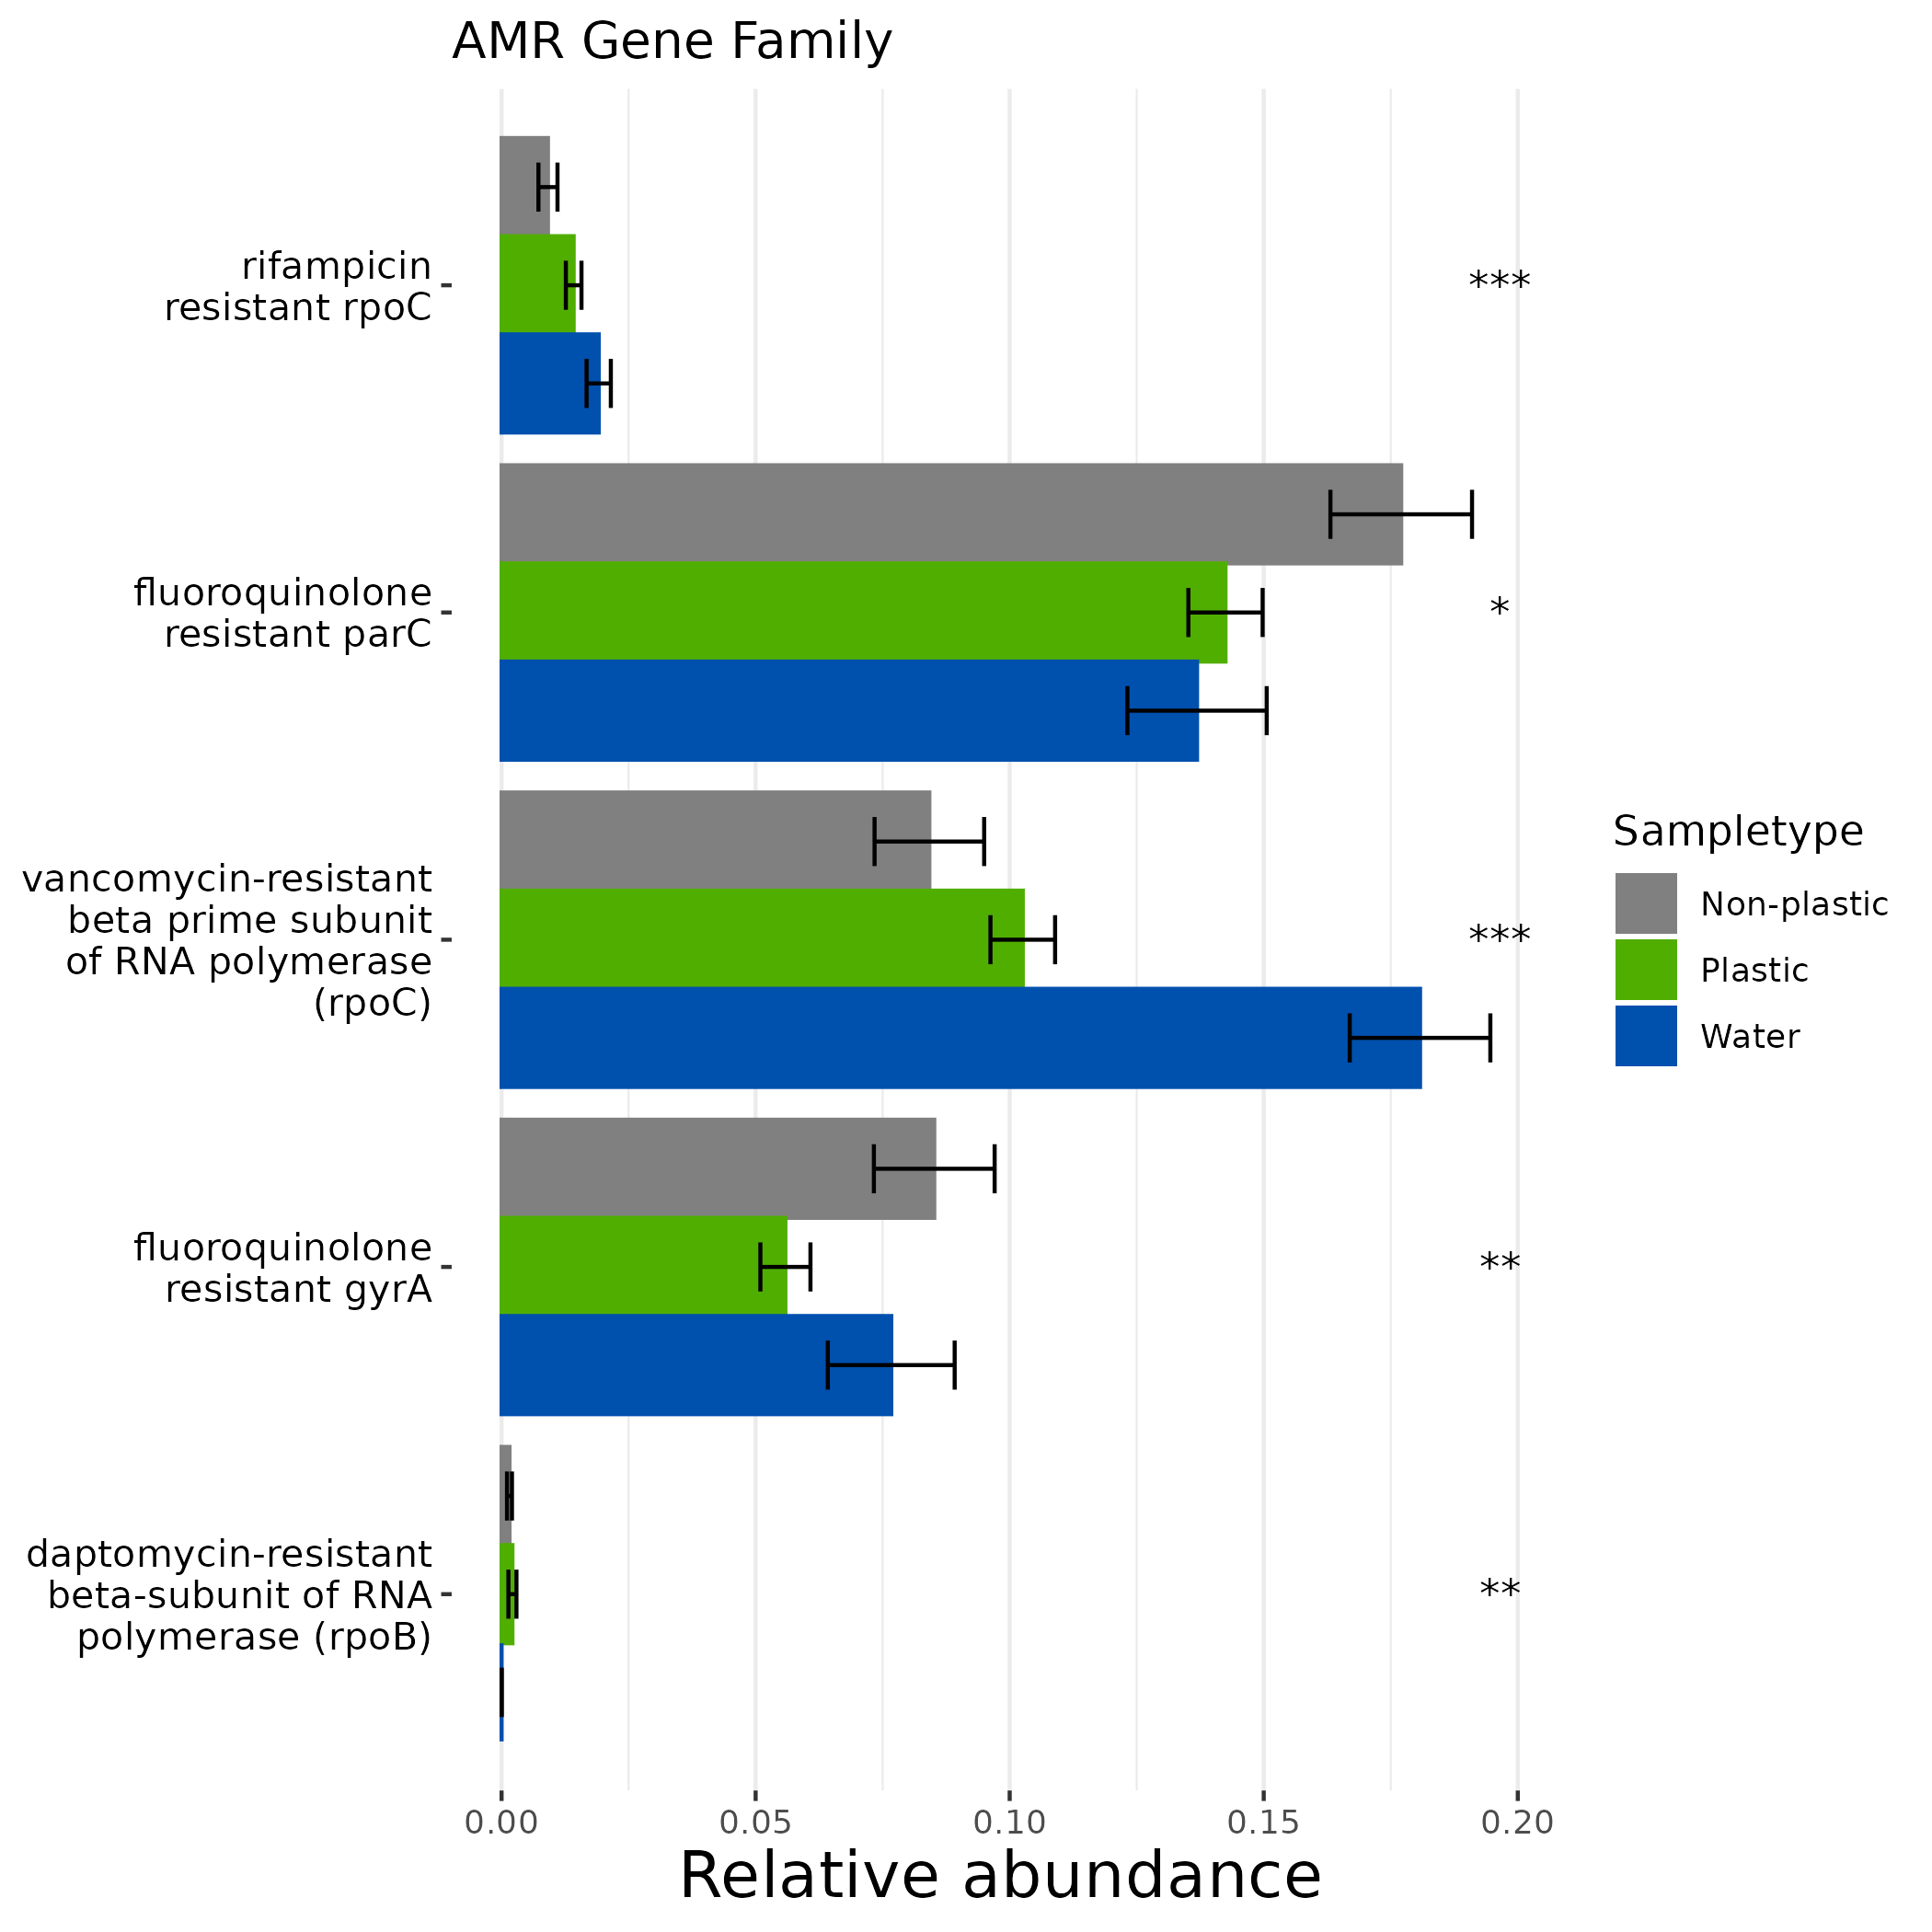
\includegraphics[width=0.5\textwidth]{figure/relative_forest_sampletype_amr_abund.png}}
    \caption{(a) Significantly assigned AMR Gene Families (Kruskal-Wallis: p < 0.05) and Mean Decrease Gini Importance when grouped by sampletype in the random forest analysis. (b) Relative Abundances of the different AMR Gene Families in the sampletype, Kruskal-Wallis: * = p < 0.05, ** = p < 0.01, *** = p < 0.001}
    \label{amr_sampletype}
\end{figure}

If instead the samples were grouped by substrate type, as shown in Figure \ref{amr_substrate_bar}, there were a lot more AMR gene families which distinguished the samples in one group from another.
Both freshwater (rifampicin, rpoC; elfamycin, EF-Tu) and seawater (vancomycin, rpoC) may be identified. The plastic susbtrates HDPE, PBSA, and PHA also had AMR gene families which distinguish them.
%The most prevalent substrate in this figure was the activated sludge, which had four different AMR Gene Families that distinguished it.
%The one labelled Multiple Resistant Variants has been renamed from "ATP-binding cassette (ABC) antibiotic efflux pump; General Bacterial Porin with reduced permeability to beta-lactams; major facilitator superfamily (MFS) antibiotic efflux pump; resistance-nodulation-cell division (RND) antibiotic efflux pump". 
%\{comment or just observation?}
All Mean Decrease Gini impurity values were positive for this grouping, there were no significant AMR Gene Families which indicated that a sample was not from a specific substrate as was the case with the water sampletype. 

\begin{figure}[!h]
    \centering
    \subfloat[\label{amr_substrate_bar}]{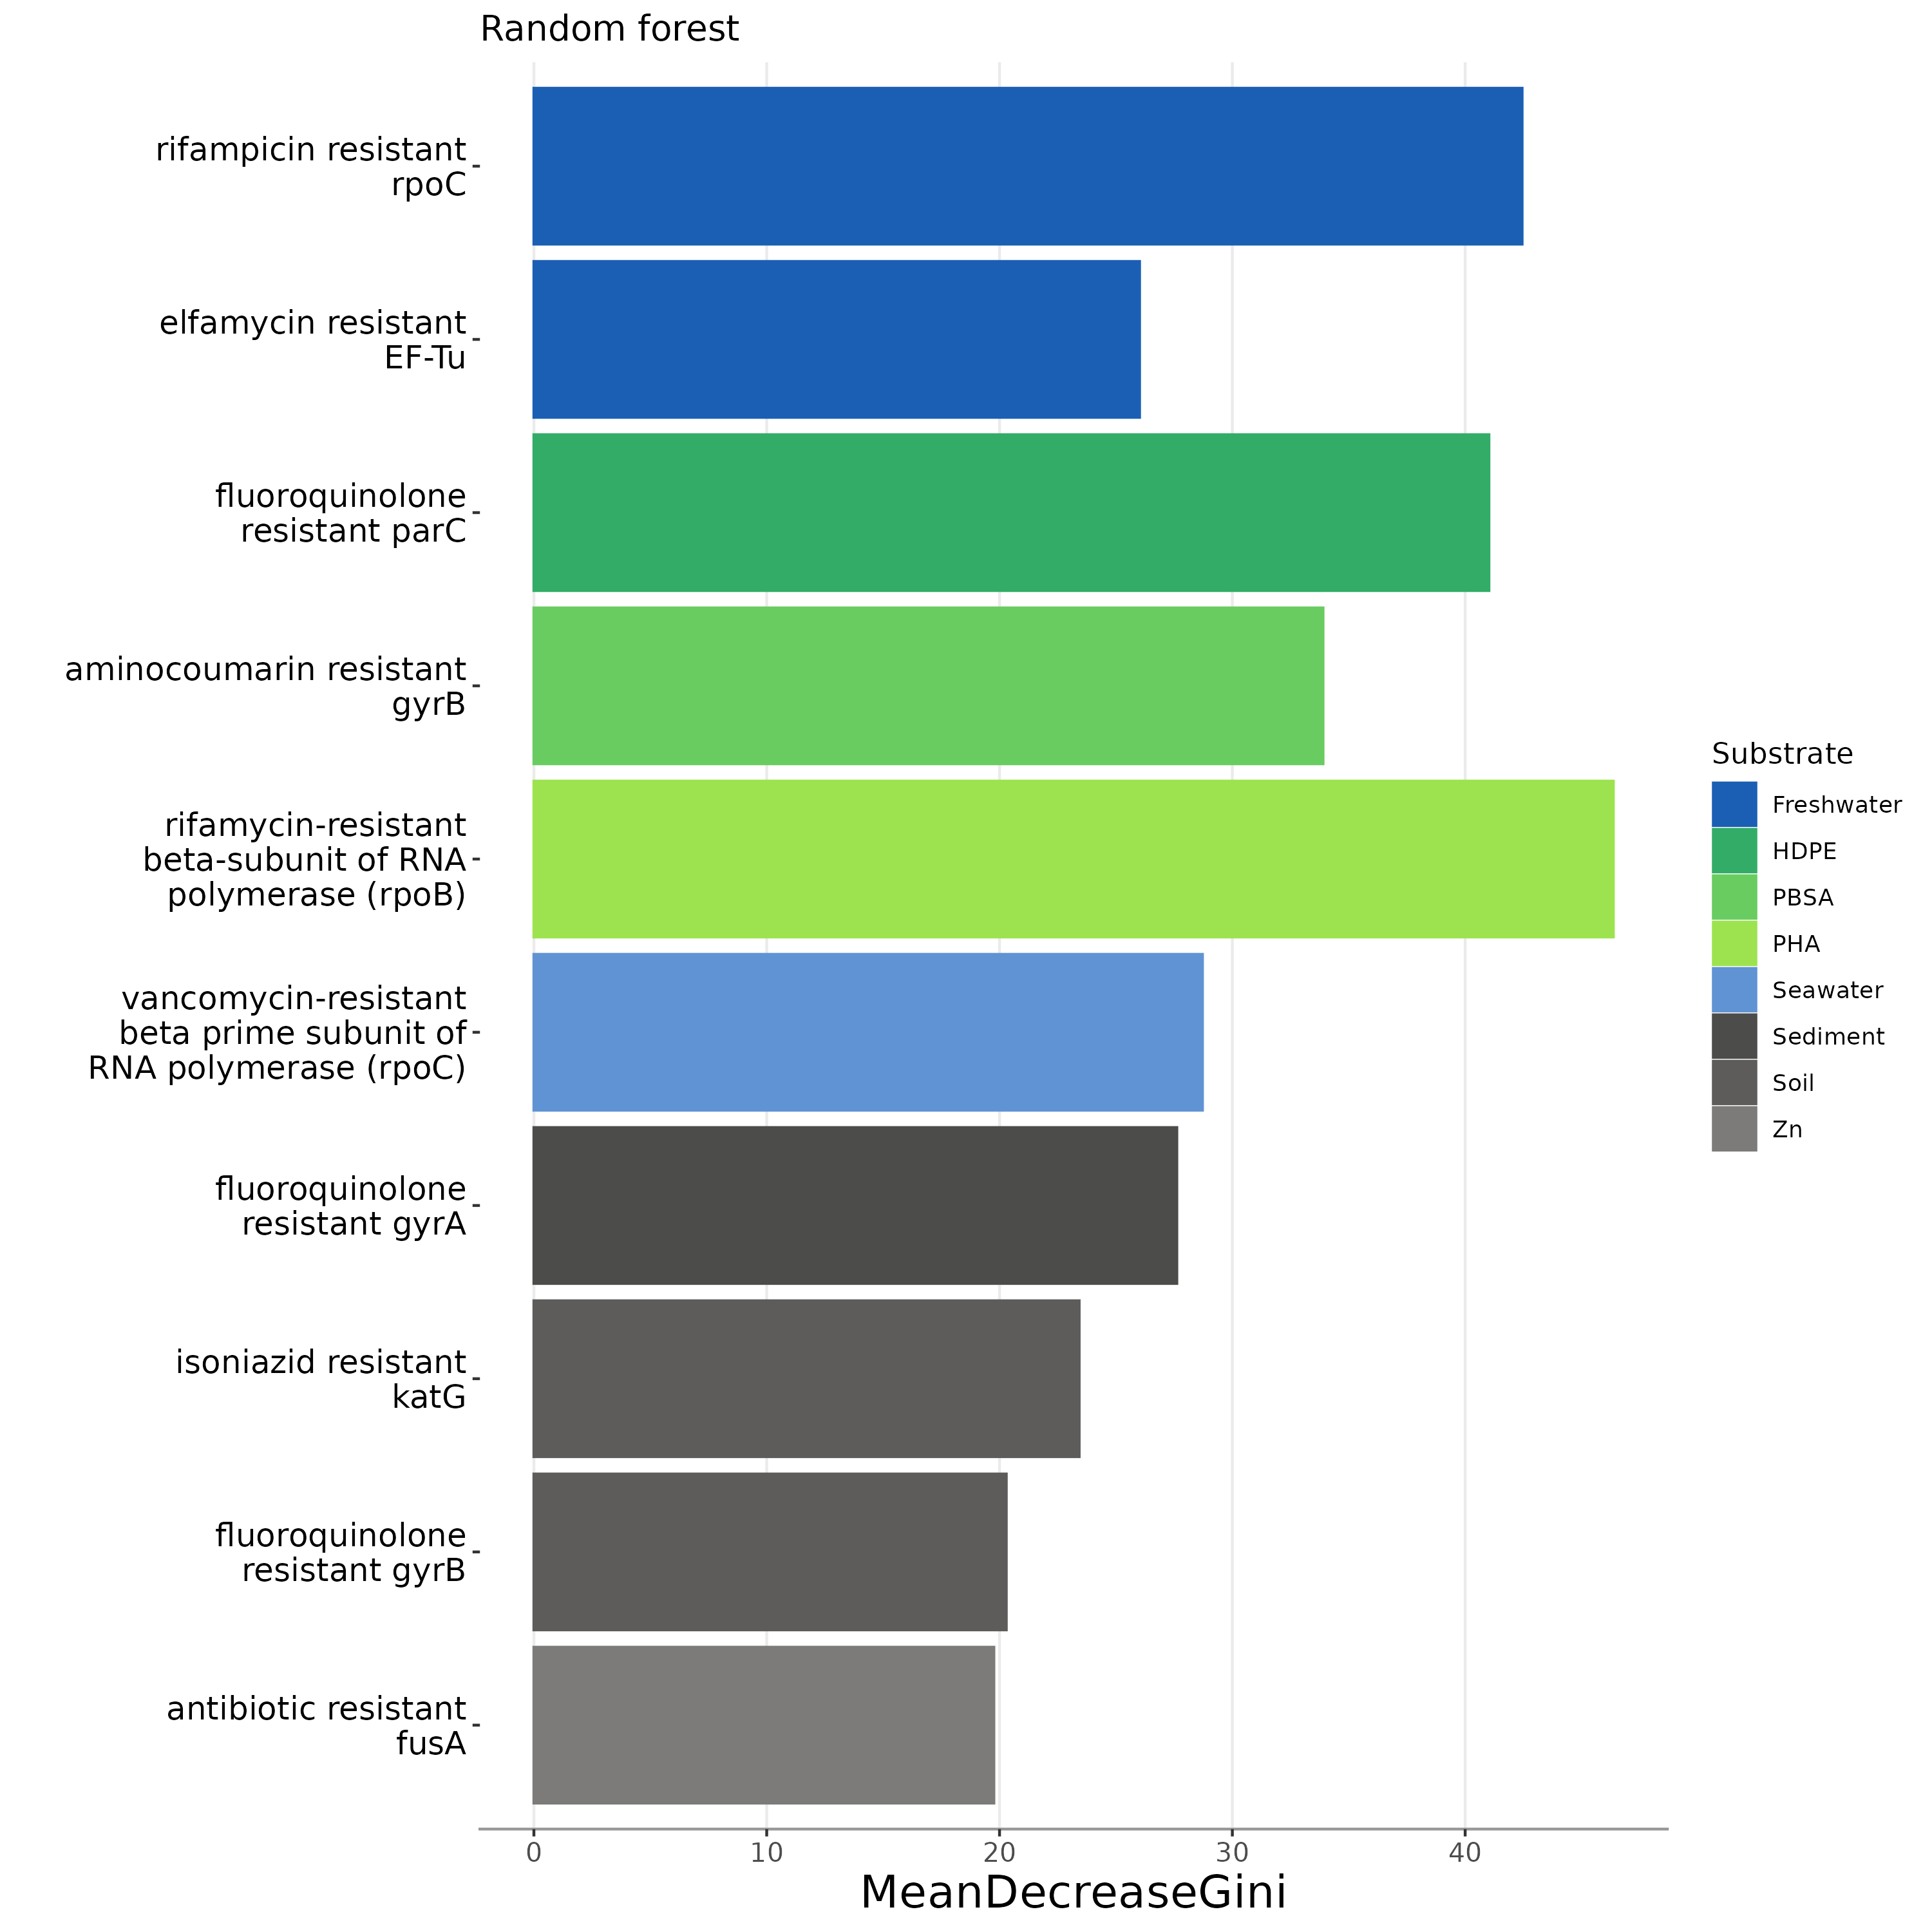
\includegraphics[width=0.5\textwidth]{figure/relative_forest_substrate_amr_bar.png}}
    \subfloat[\label{amr_substrate_abund}]{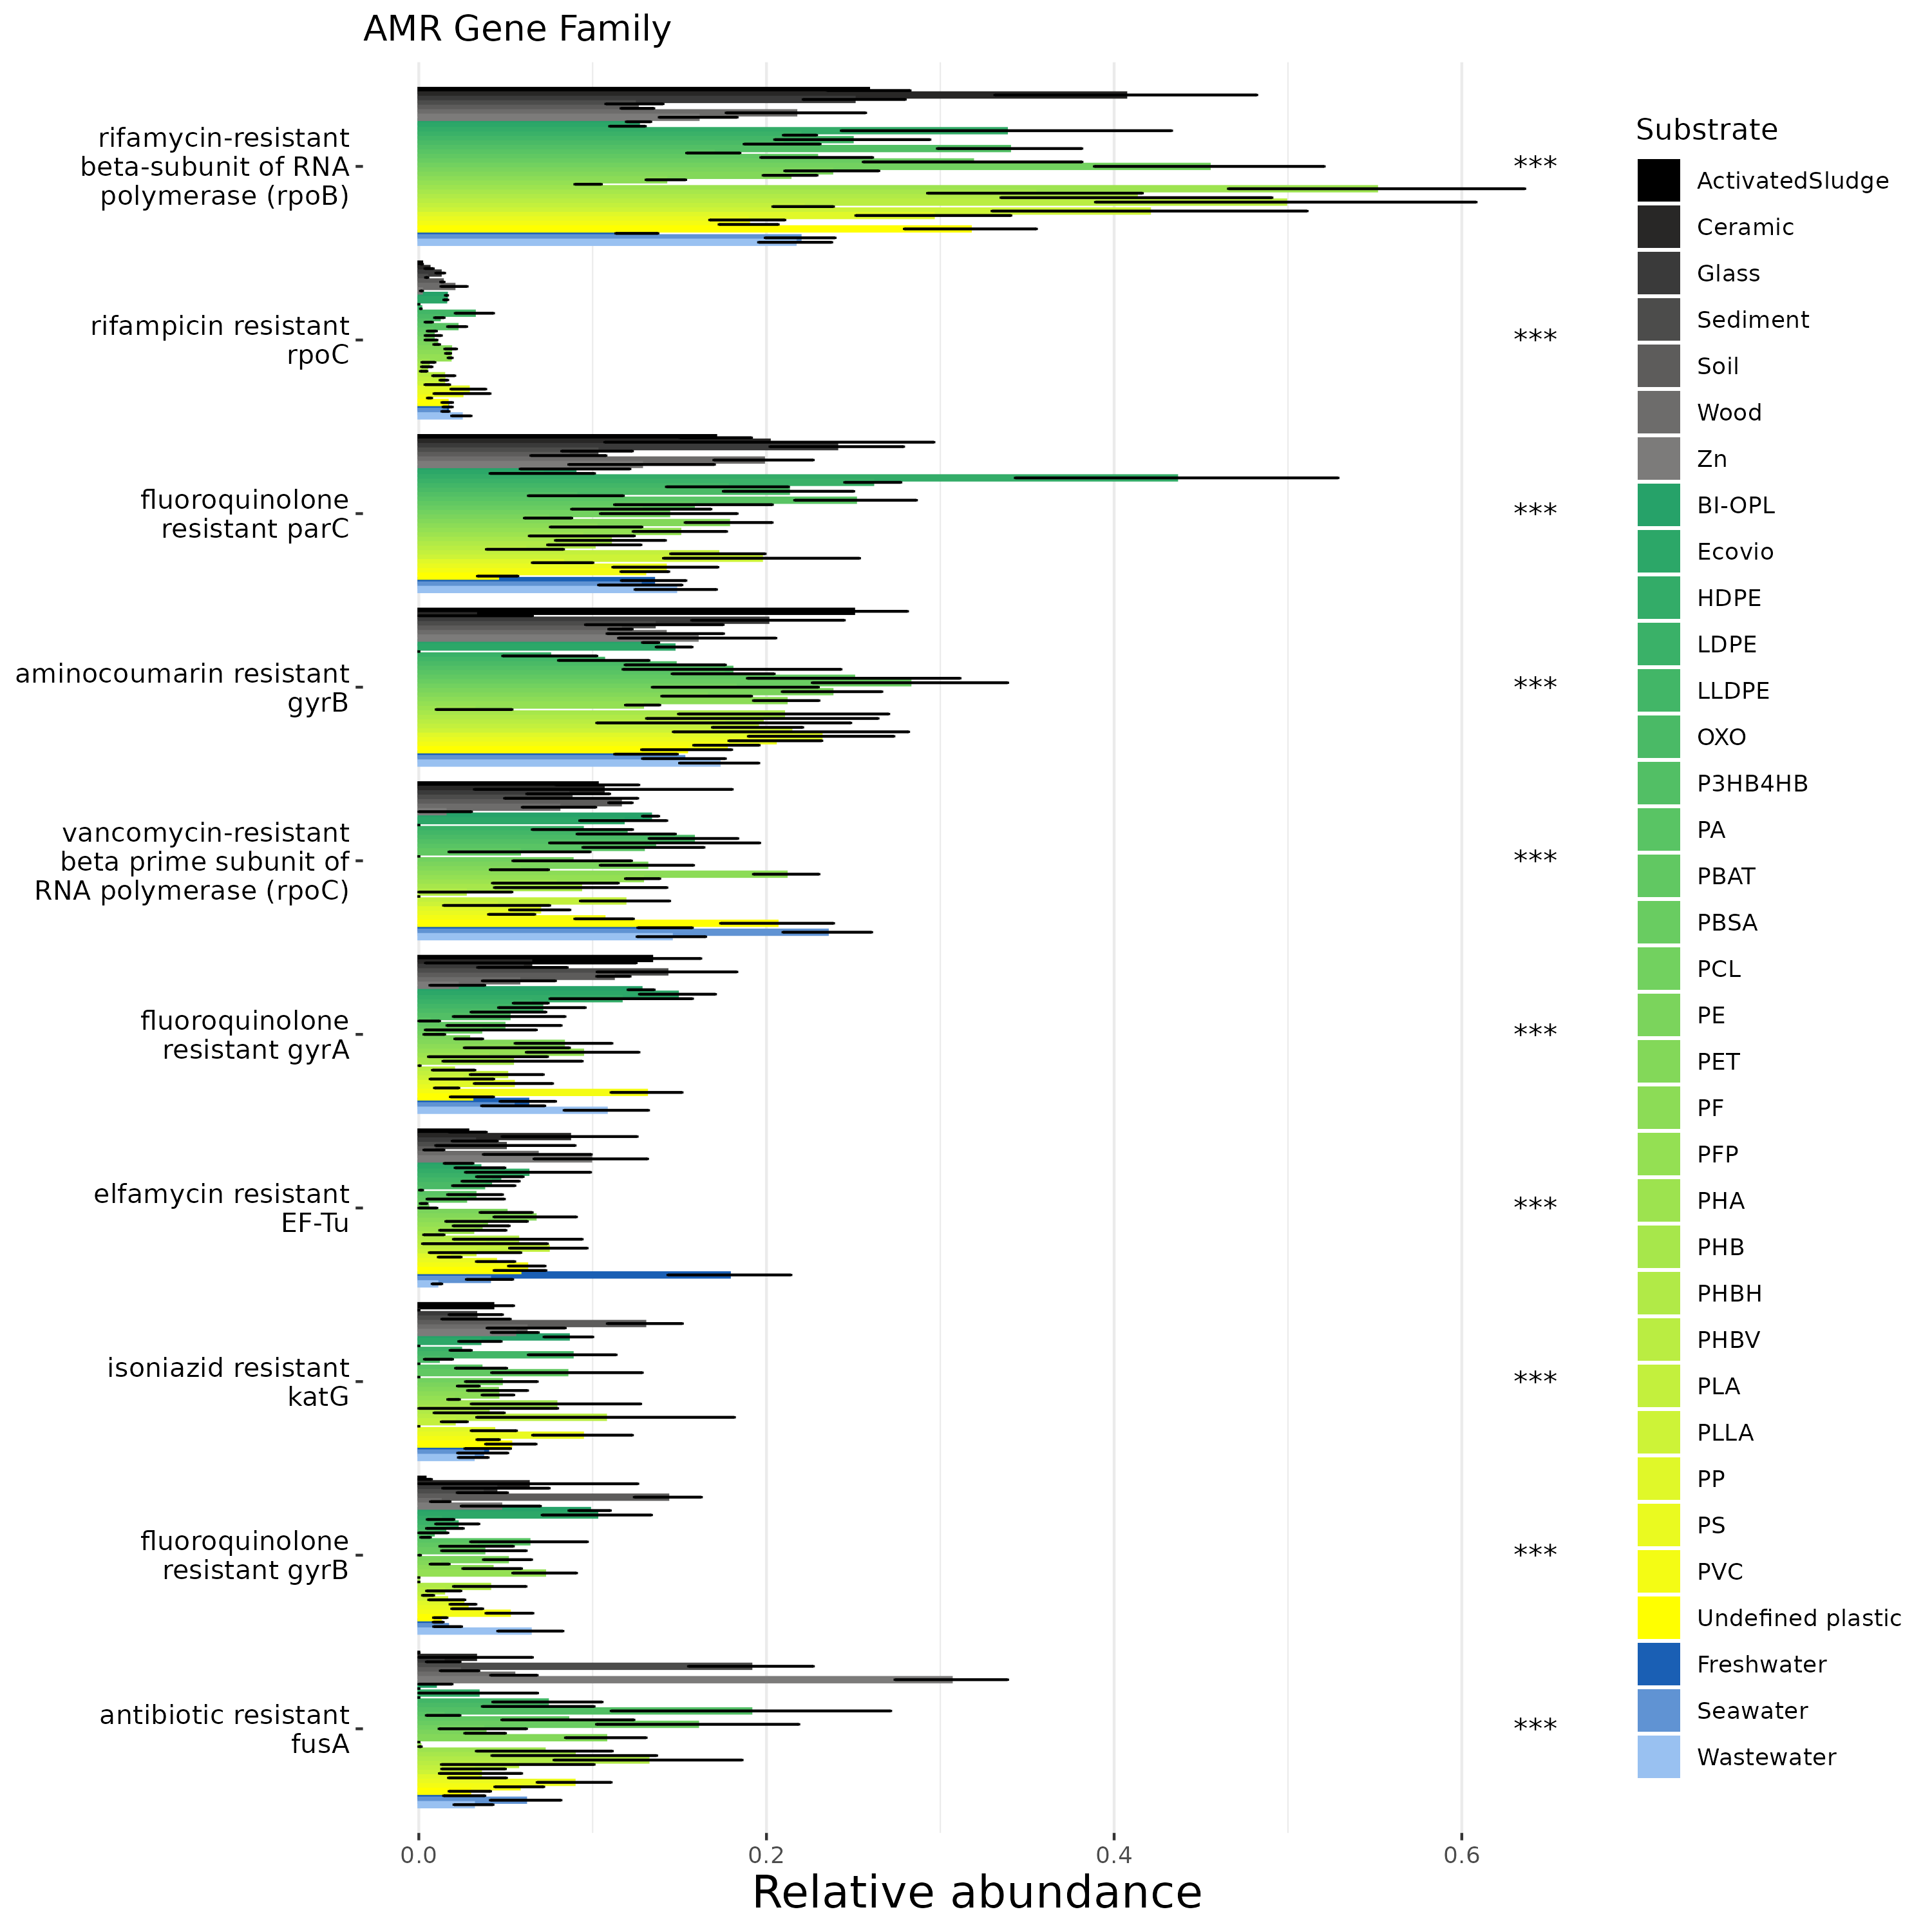
\includegraphics[width=0.5\textwidth]{figure/relative_forest_substrate_amr_abund.png}}
    \caption{(a) Significantly assigned AMR Gene Families (Kruskal-Wallis: p < 0.001) and Mean Decrease Gini Importance when grouped by substrate in the random forest analysis. (b) Relative Abundances of the different AMR Gene Families in the substrates, Kruskal-Wallis: *** = p < 0.001}
    \label{amr_substrate}
\end{figure}

\newpage
\subsection{Prediciting point mutations as substrate identifiers}
%todo{Predicting identity using point mutation} todo{Substrate prediction using point mutations} todo{Prediciting substrate identifiers using point mutations}
The following figures used the individual point mutations, or combinations thereof, found in the samples as the grouping for which the random forest analysis was performed, instead of the AMR Gene Family. 
Only the non-plastic sampletype could be significantly assigned (p < 0.05) to any mutation in Figure \ref{snps_sampletype}, which includes several mutations in rpoB which confer resistance to rifampicin, as well as several in gyrA and parC which confer resistance to fluoroquinolone. 
As for the assignment to the AMR Gene Families, the water sampletype could not be assigned to any specific point mutations directly. However one could assign a greater importance to the reference group, which consisted of the two other sampletypes, than the water group for two mutations which both occur in rpoC.

%Figure \ref{snp_sampletype_bar} show the result of the analysis using the three different sampletypes as grouping, and as above only the non-plastic group and the water group are present. 
%The significant mutations for the non-plastic group include several mutations in rpoB which confer resistance to rifampicin, as well as several in gyrA and parC which confer resistance to fluoroquinolones.
%There is one combination of four mutations in rpoB which confer resistance to rifampicin. 
%However, the abundance of these mutations is relatively low, as is shown in figure \ref{snp_sampletype_abund}.

\begin{figure}[h]
    \centering
    \subfloat[\label{snp_sampletype_bar}]{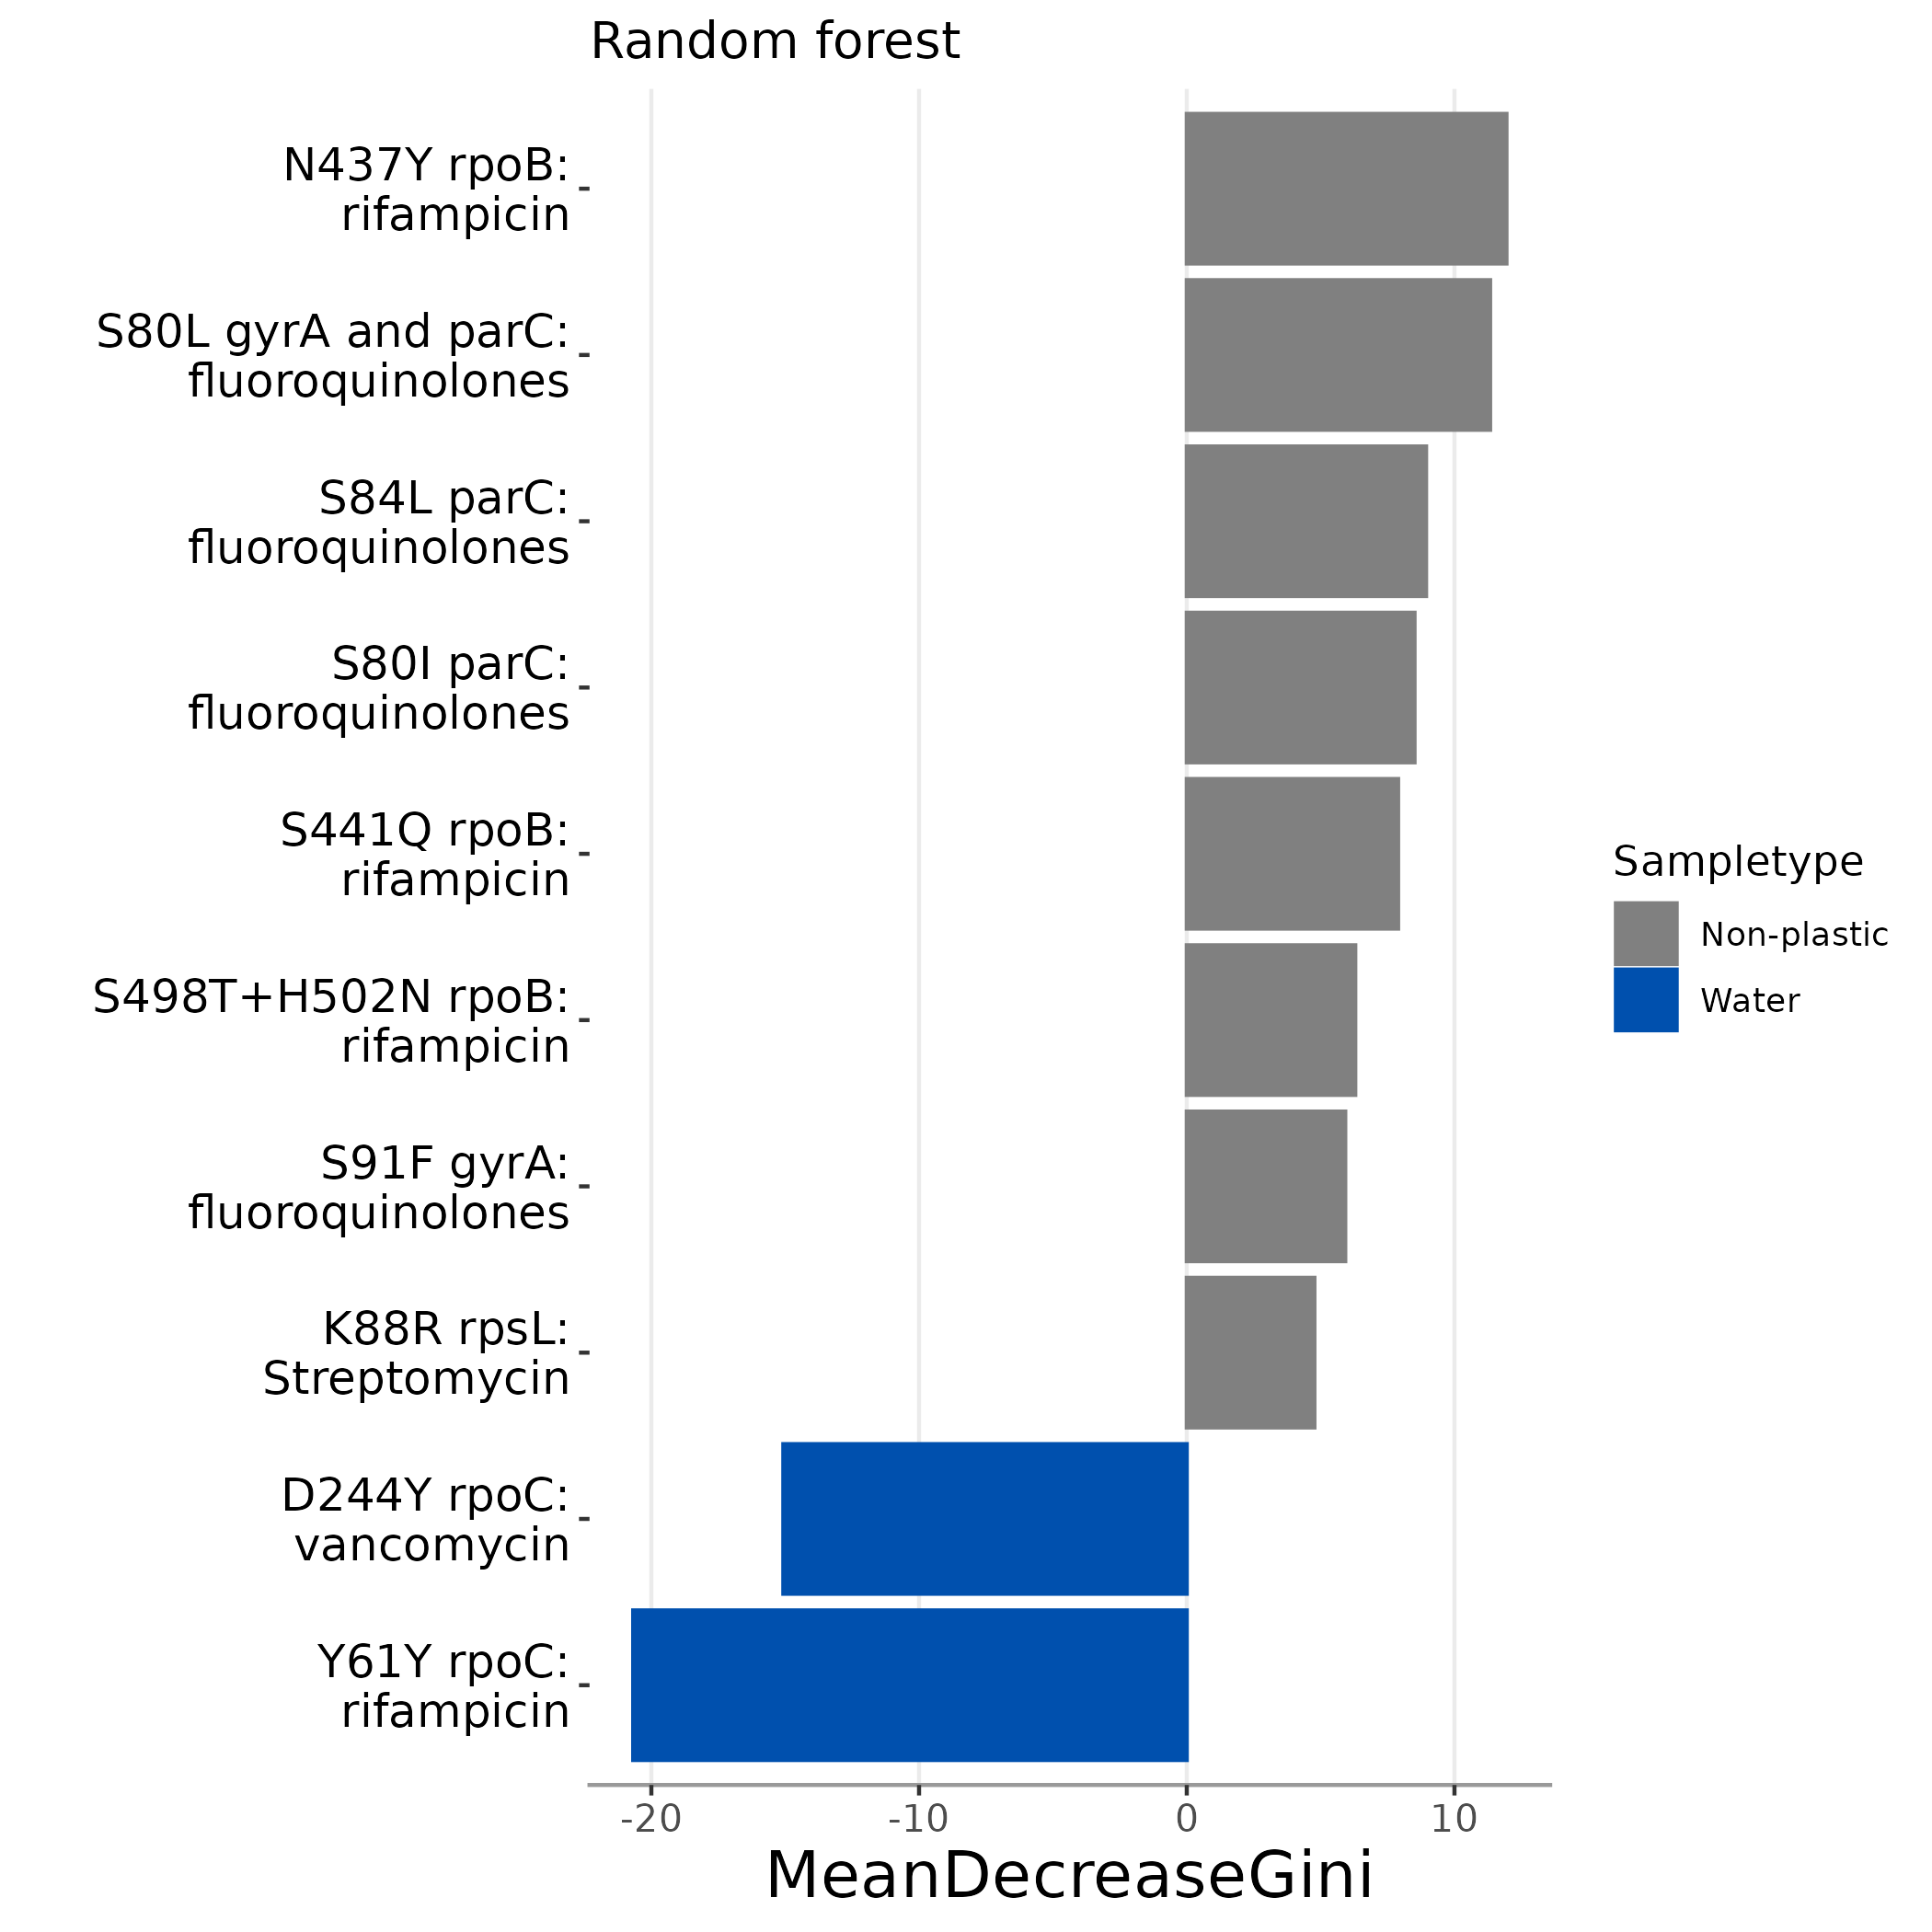
\includegraphics[width=0.5\textwidth]{figure/relative_forest_sampletype_snps_bar.png}}
    \subfloat[\label{snp_sampletype_abund}]{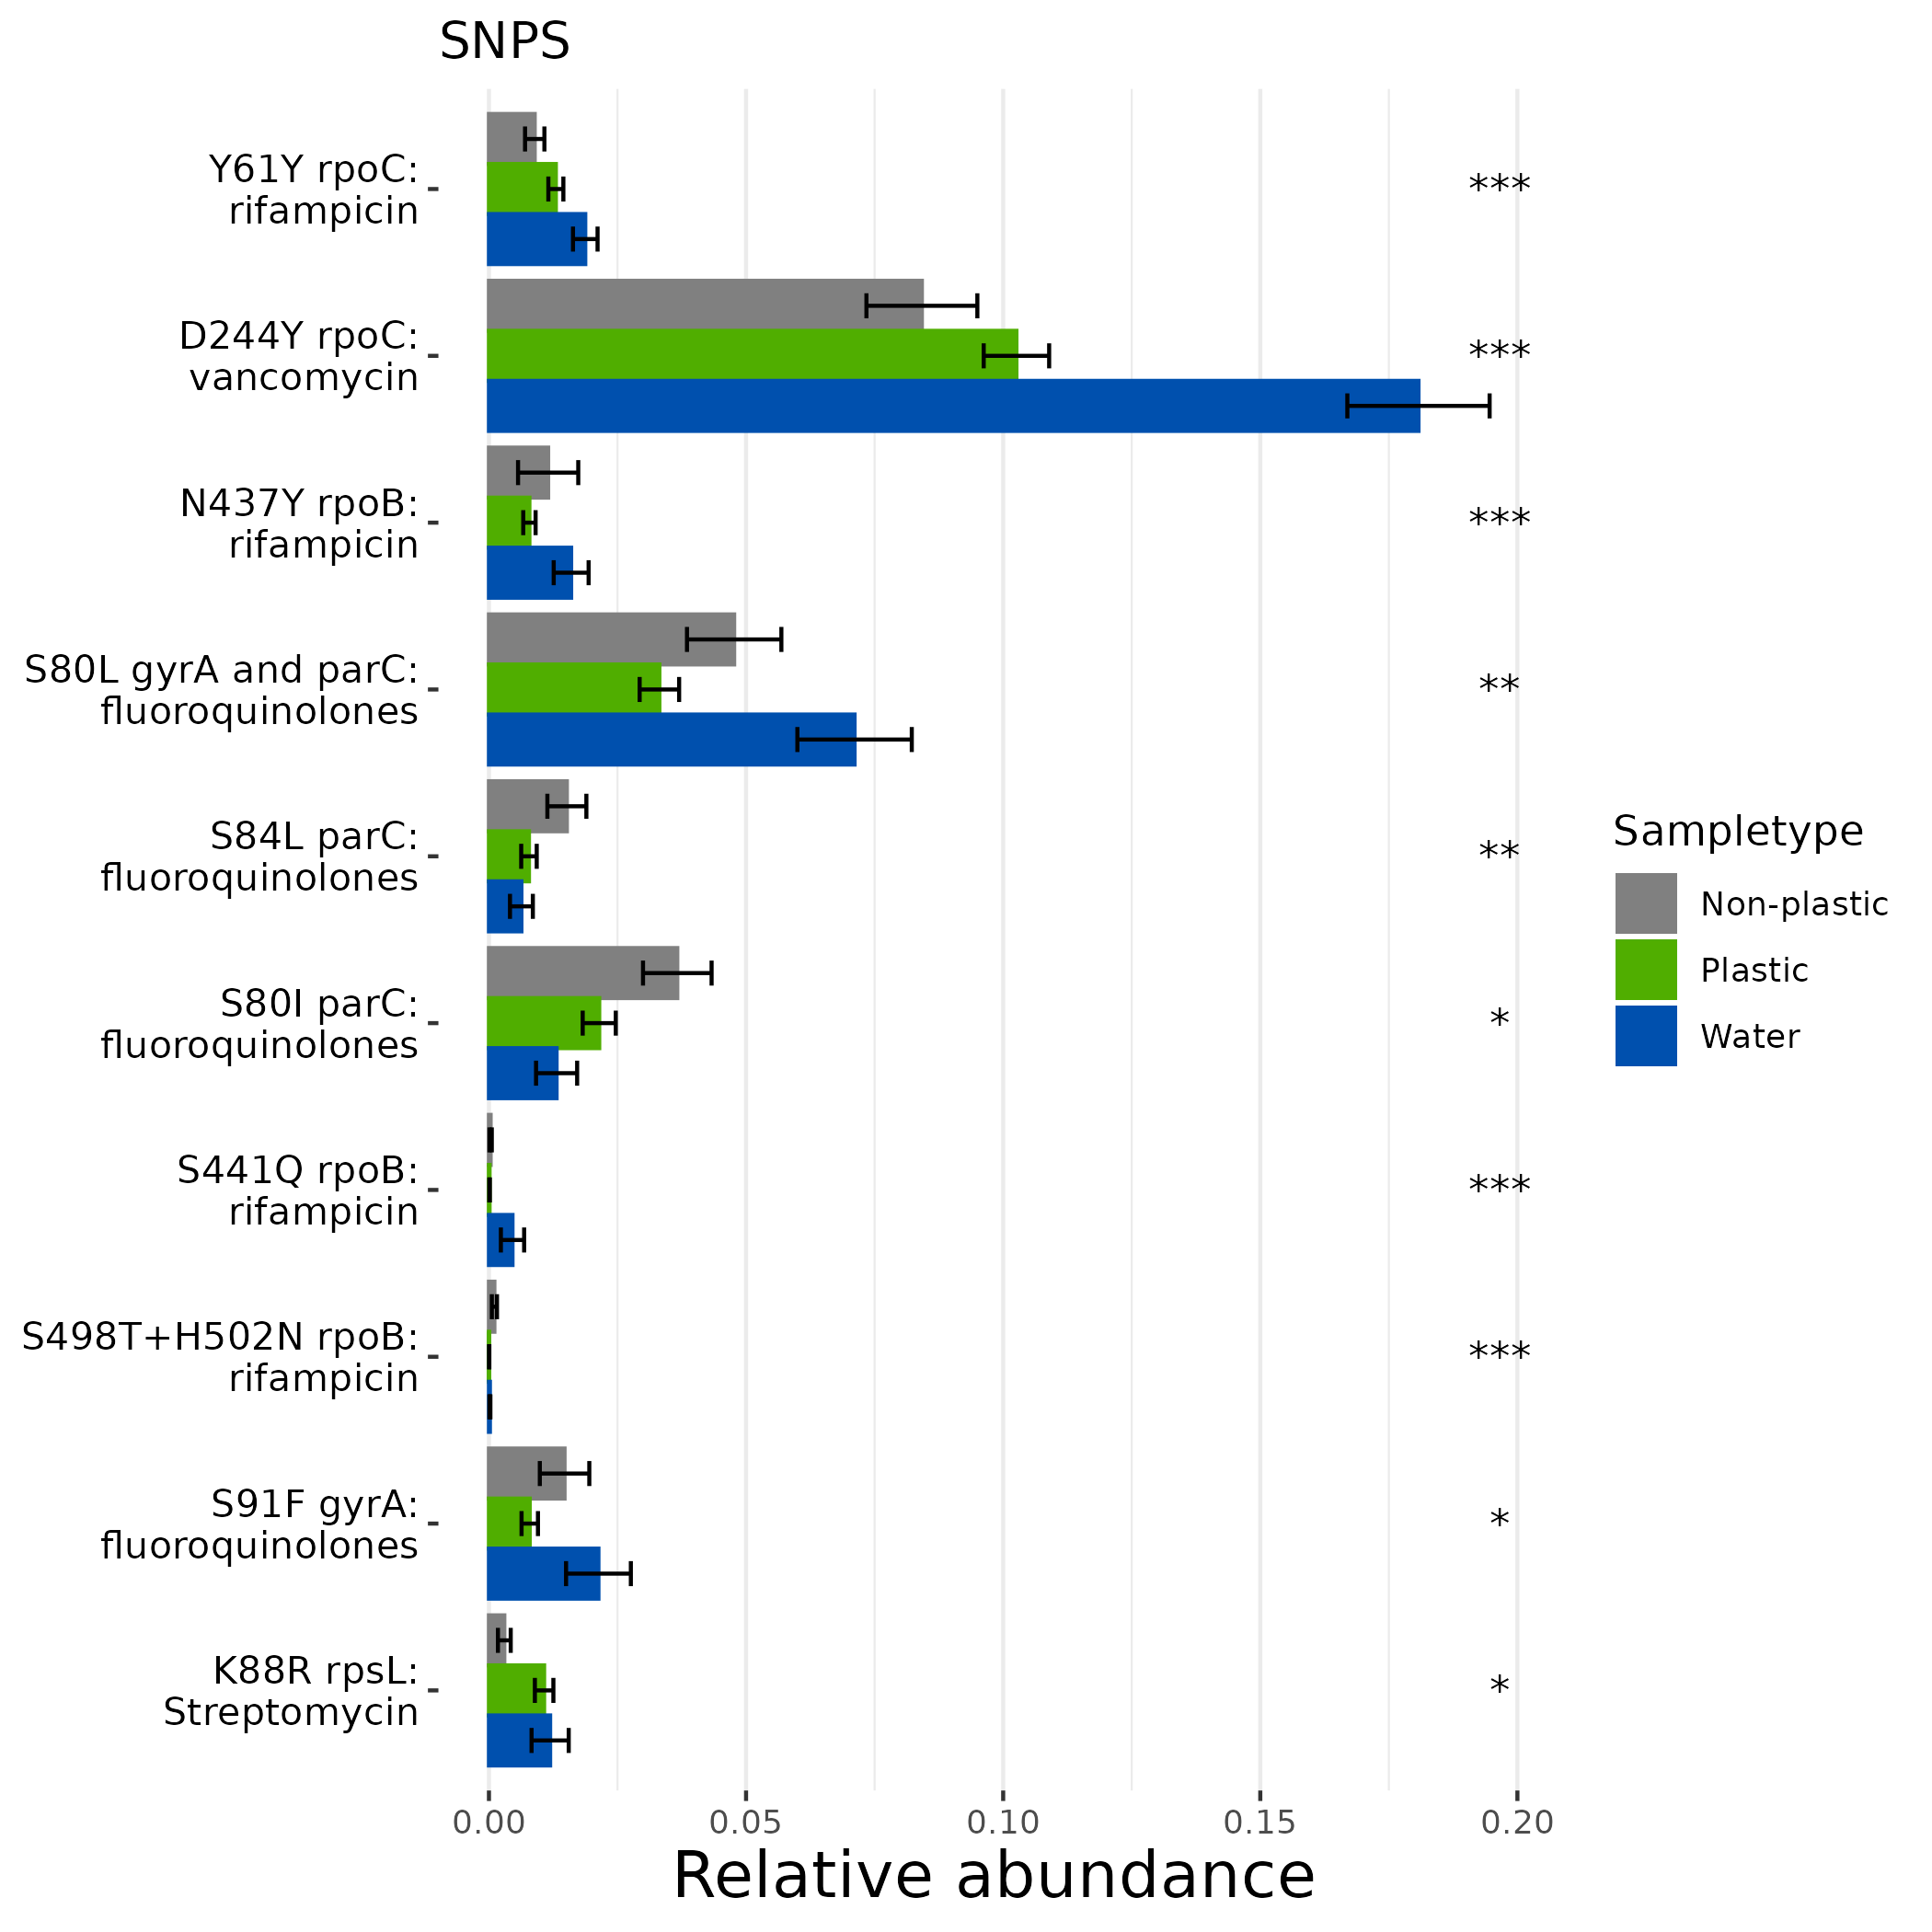
\includegraphics[width=0.5\textwidth]{figure/relative_forest_sampletype_snps_abund.png}}
    \caption{(a) Significantly assigned point mutations (Kruskal-Wallis: p < 0.05) and Mean Decrease Gini Importance when grouped by sampletype in the random forest analysis. (b) Relative Abundances of the different point mutations in the sampletype, Kruskal-Wallis: * = p < 0.05, ** = p < 0.01, *** = p < 0.001}
    \label{snps_sampletype}
\end{figure}

When instead the different substrates was used as the grouping variable in the random forest analysis, the mutations with the highest mean decrease Gini importance were not the same, however many of the genes and the resistances they confer were. These included parC (fluoroquinolones), rpoB (rifampicin), rpoC (rifampicin or vancomycin), gyrB (aminocoumarin), and are shown in Figure \ref{snp_substrate_bar}. The mutations in EF-Tu, which confer resistance to pulvomycin, are not present in the previous plot, and may be used to identify ceramic as a substrate. Note however that there were only three ceramic samples in this study, which may skew the results.

\begin{figure}[h!]
    \centering
    \subfloat[caption1.\label{snp_substrate_bar}]{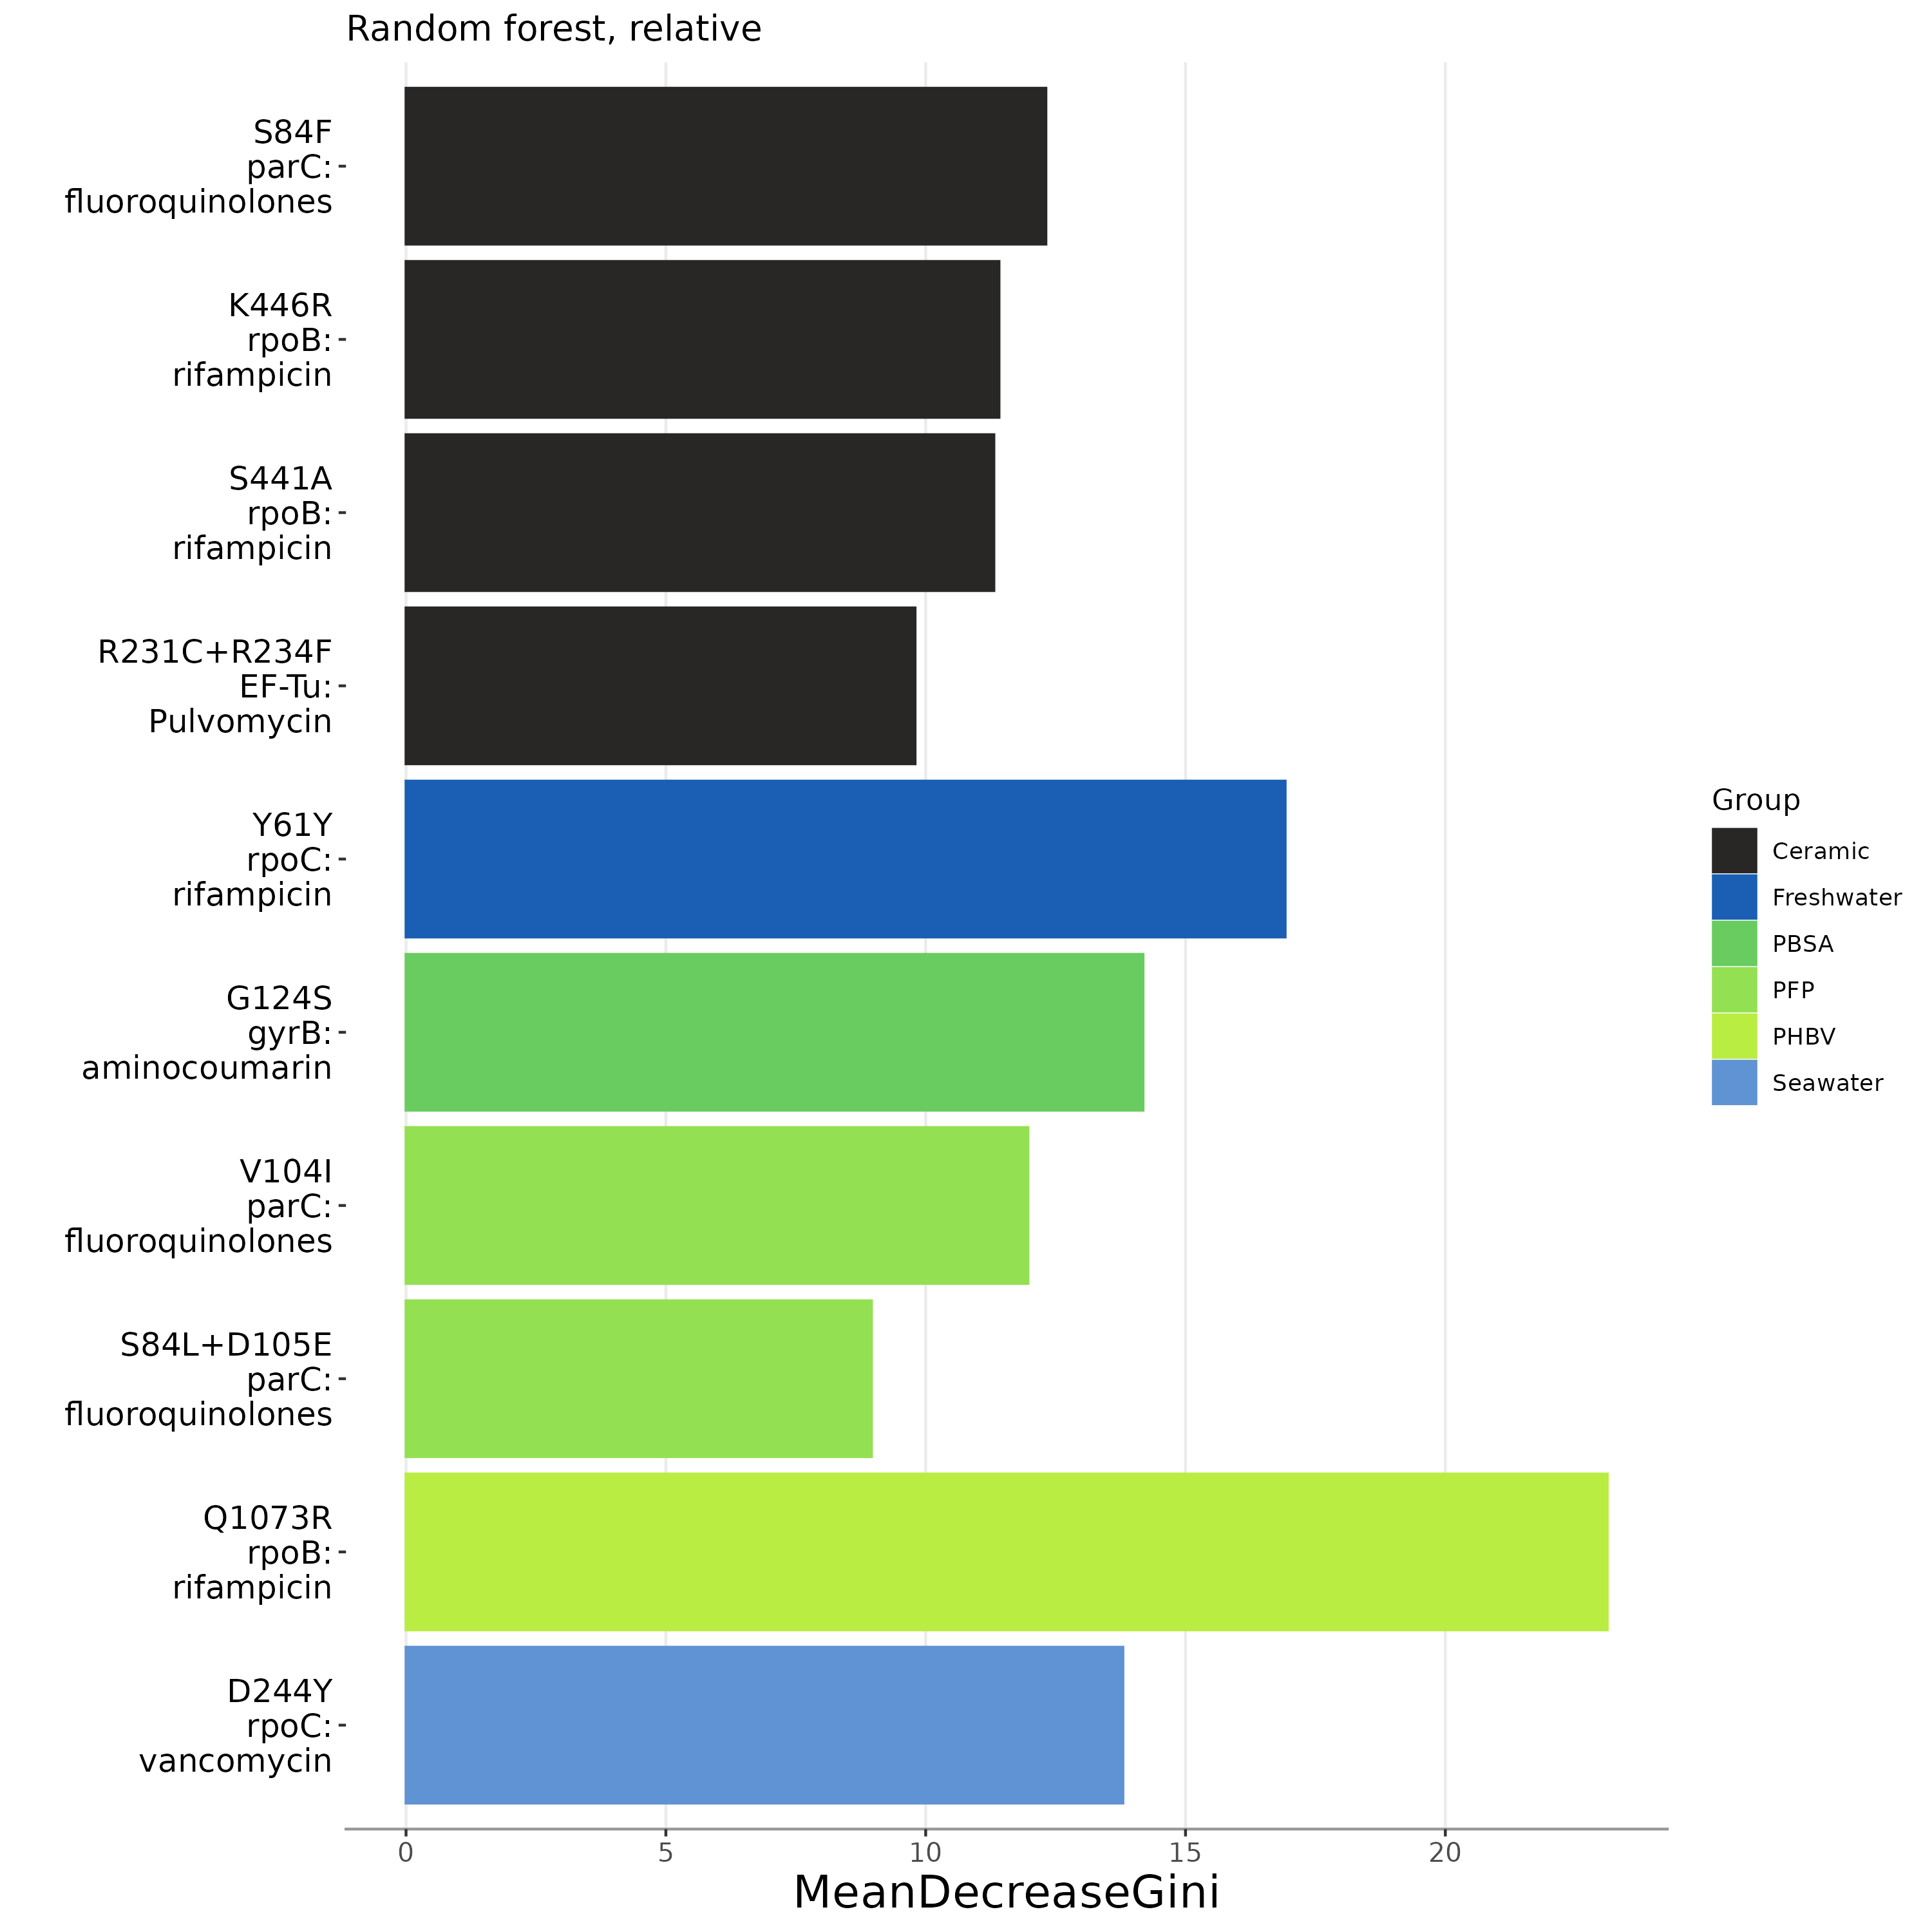
\includegraphics[width=0.5\textwidth]{figure/relative_forest_substrate_snps_bar.png}}
    \subfloat[caption2.\label{snp_substrate_abund}]{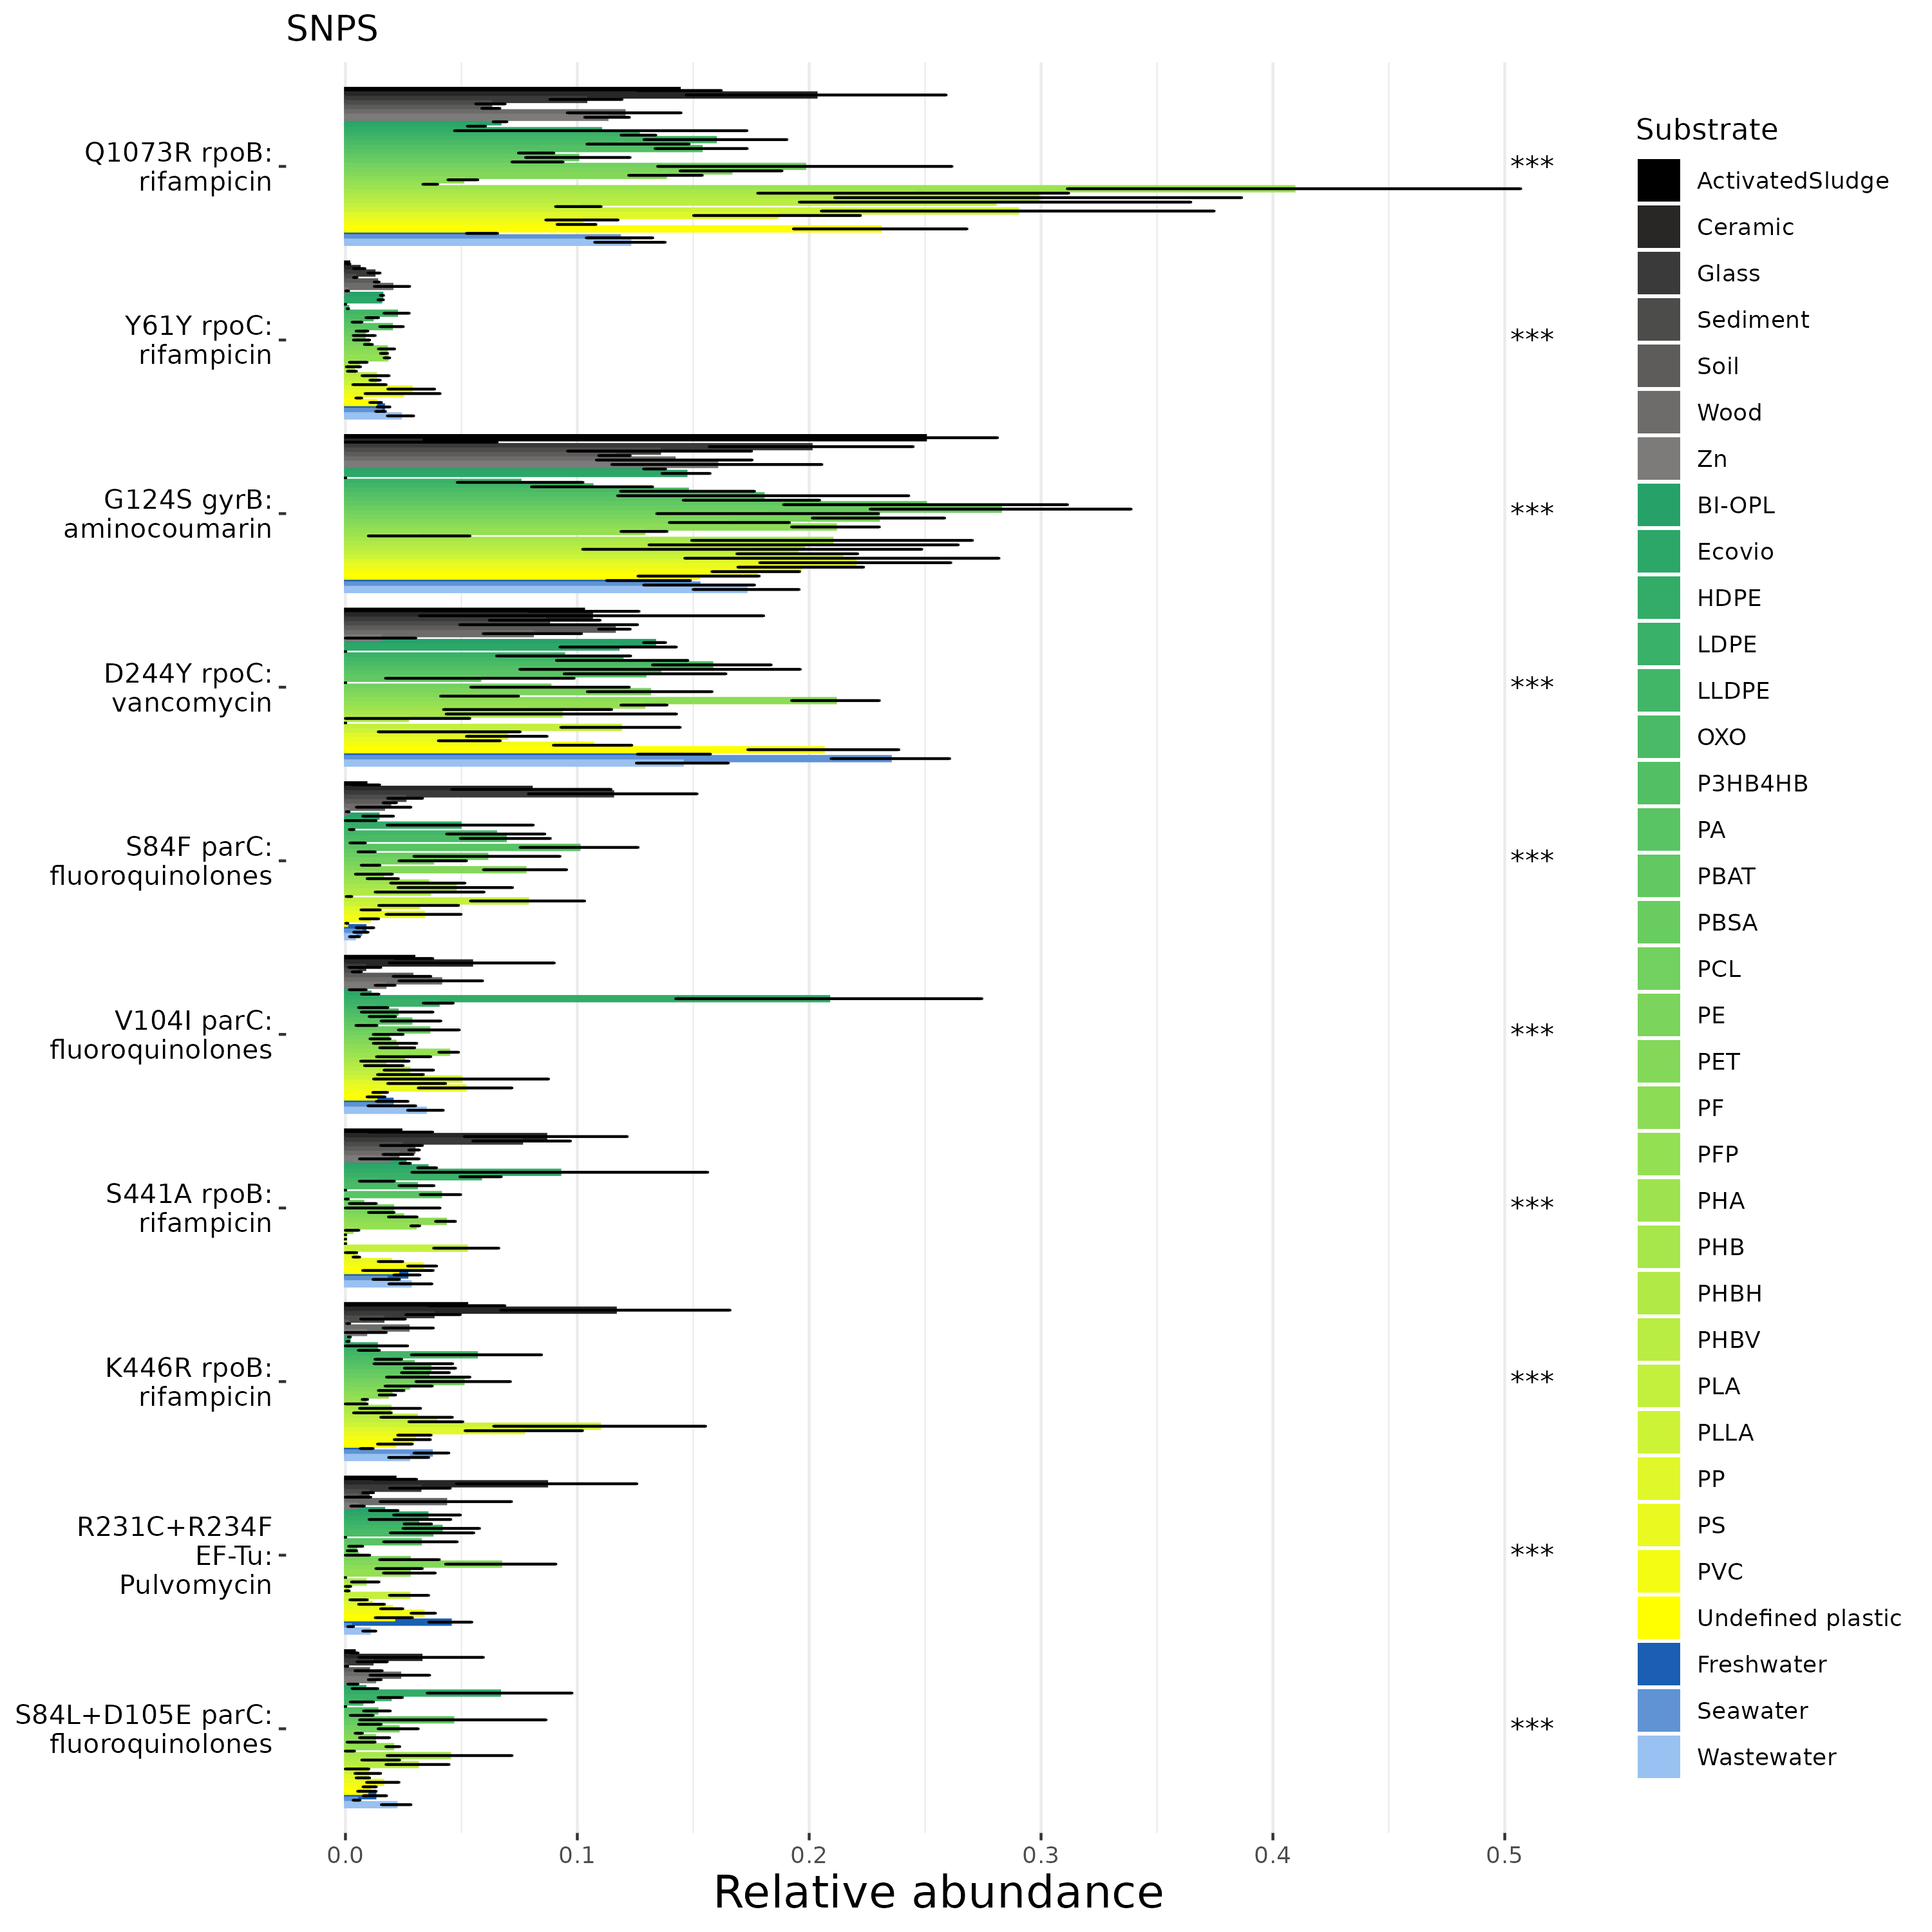
\includegraphics[width=0.5\textwidth]{figure/relative_forest_substrate_snps_abund.png}}
    \caption{(a) Significantly assigned point mutations (Kruskal-Wallis: p < 0.001) and Mean Decrease Gini Importance when grouped by substrate in the random forest analysis. (b) Relative Abundances of the different point mutations in the substrate, Kruskal-Wallis: *** = p < 0.001}
    \label{snps_substrate}
\end{figure}

\newpage
\section{Taxonomic Composition}
The relative abundance of bacterial phyla is shown in Figure \ref{tax_plot}.
%The plot show the taxonomic composition at the phylum level, and is divided by ecosystem type and sampletype. 
%Only the eight most abundant phyla has been included, where the rest has been grouped into "Others".
%The ecosystem type is the environment in which the sample was taken, regardless of the sampletype. For example, some of the samples were taken in the Pacific Ocean, and there both plastic substrates and seawater substrates were analysed.
%The figure shows that the largest difference is between the different ecosystems, but that sampletype also matters.\{Very unsure of how to analuze these plots, since we lack statistics for them.}
The most abundant phyla in all ecosystems were \emph{Proteobacteria}, except in the wastewater samples where SAR was most abundant in most of the samples.
Other abundant phyla were \emph{Archaeplastida} in the PE samples from the marine ecosystems, see \ref{tax_plot_substrate_flip}, \emph{Amorphea} in the Undefined plastic samples and in PVC from wastewater. The soil and sediment samples contained a large proportion of other phyla (such as \emph{Chloroflexi}, \emph{Verrucomicrobiota}, and \emph{Planctomycetota}) which were not part of the eight most abundant ones presented in Figure \ref{tax_plot}.

%into which the phyla not part of the eight most abundant ones are grouped. 
% Soil:
%-Proteobacteria
%-Actinobacteriota
%-Amorphea
% Chloroflexi
% Verrucomicrobiota
% Planctomycetota
% Acidobacteriota
%-Bacteriodota
%-Others

%wastewater: Archaeplastida (Some ocean plastic samples, the PE ones)
%Plastic and wastewater: Amorphea (plastic: undefined, from great pacific garbage patch; wastewater: PVC)
%Soil and sediment: >50\% others

%there are differences between the different ecosystems, but that there is relatively small differences between the different sampletypes and substrates. 

%Figure \ref{tax_plot_substrate} show the same plot, but this time also divided by substrate.\{Which of these should be present? Could turn the whole plot 90° on the page to be easier to read? see fig \ref{tax_plot_substrate_flip}}

\begin{figure}[h]
    \centering
    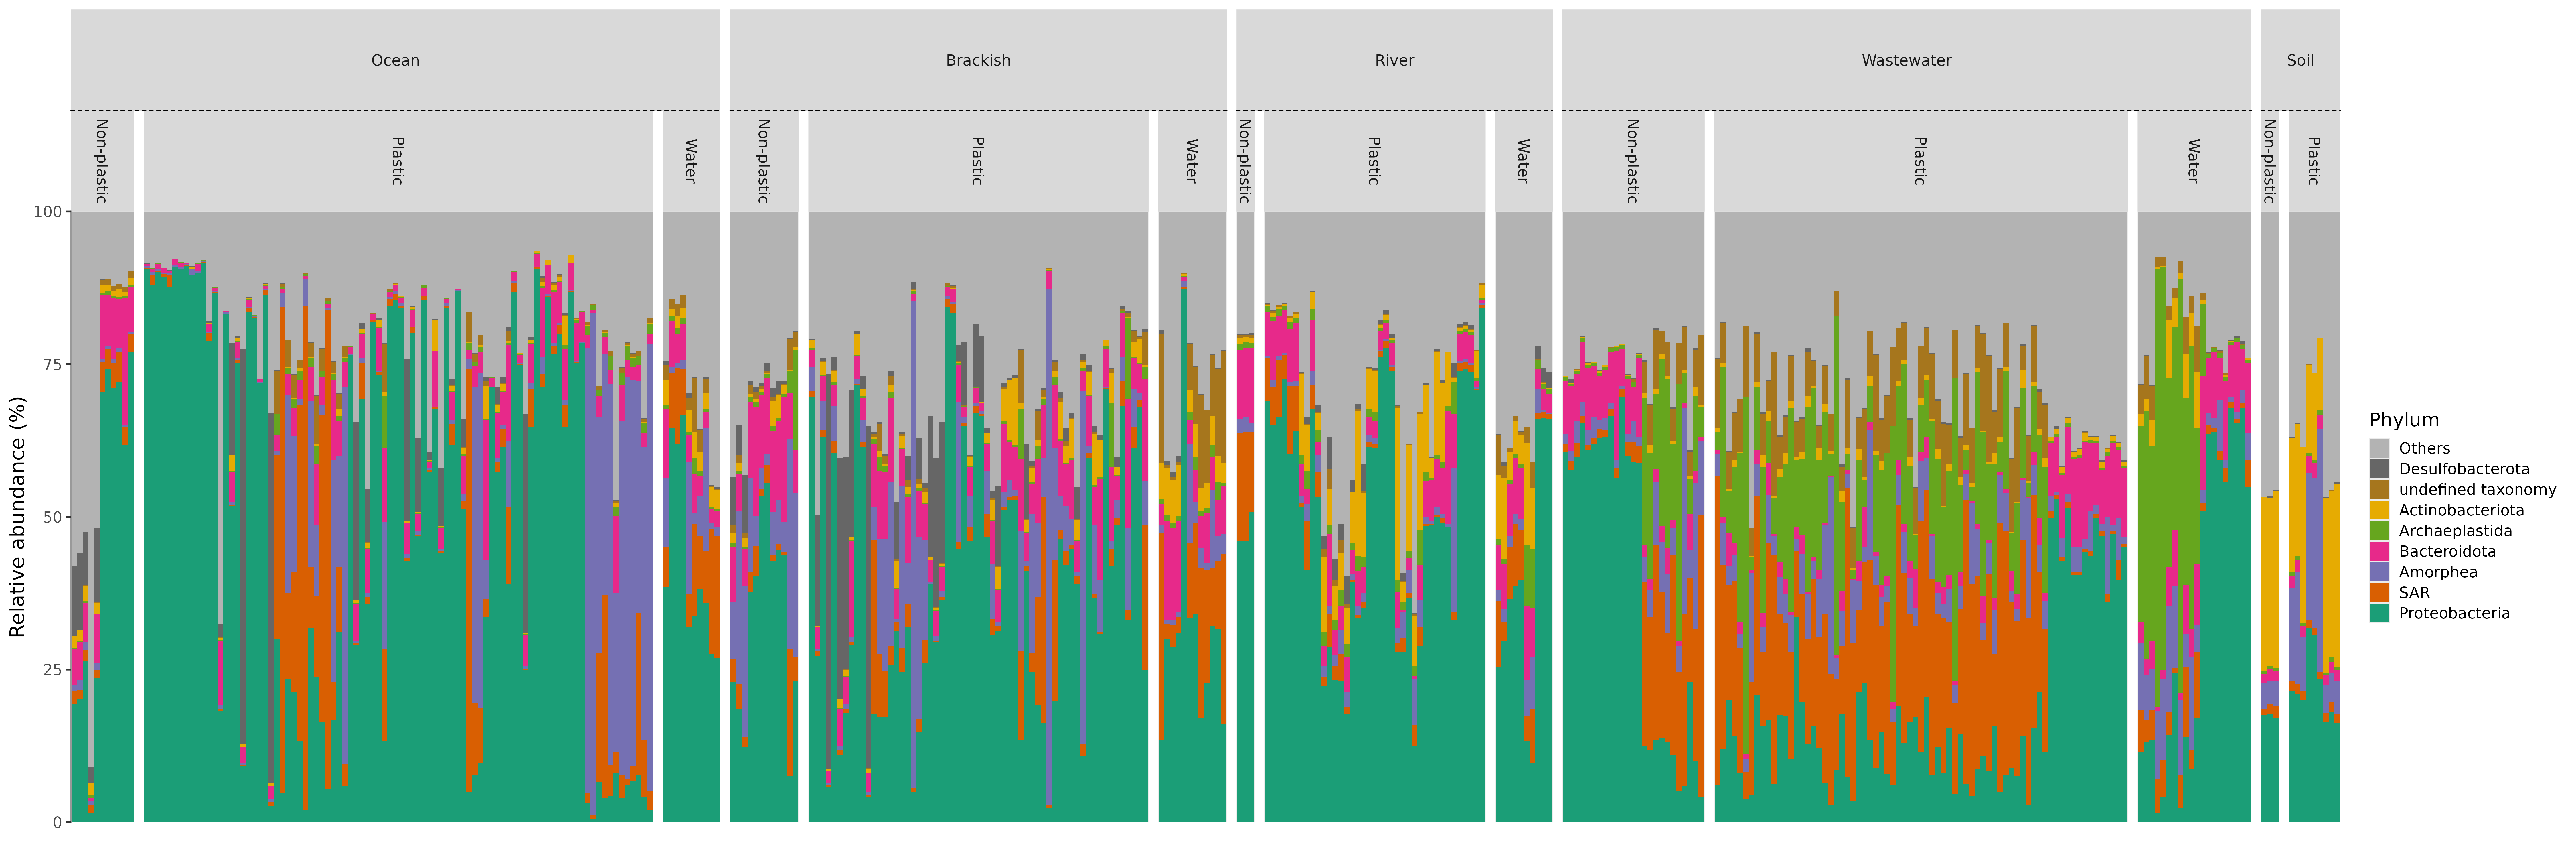
\includegraphics[width = 0.9\textheight, angle = 90]{figure/tax_phylum_ecosystem_sampletype.png}
    \caption{Taxonomic composition for all samples showing the top 8 phyla, divided by ecosystem type and sampletype. Only the eight most abundant phyla has been included, where the rest has been grouped into "Others".}
    \label{tax_plot}
\end{figure}












